%\documentclass{sig-alternate}
%\documentclass{acm_proc_article-sp}
\documentclass[a4paper,english]{article}

\makeatletter
\newif\if@restonecol

\let\algorithm\relax
\let\endalgorithm\relax
\usepackage[tight,footnotesize]{subfigure}
\usepackage {paralist}
\usepackage{comment}
\usepackage{array}
\usepackage{amsmath}
\usepackage{graphicx}
\usepackage{amssymb}
\usepackage{cite}
\usepackage{url}
\usepackage{changepage}
\makeatother
\makeatletter
\usepackage[ruled]{algorithm2e}
\providecommand{\tabularnewline}{\\}


\newtheorem{clm}{Claim}
\newtheorem{proof}{Proof}
\newtheorem{mydef}{Definition}
\begin{document}

\title{On the design of real-time STM contention managers%\thanks{\footnotesize{Approved for Public Release. Unlimited Distribution.}}
}


\author{Mohammed El-Shambakey, Binoy Ravindran\\
ECE Dept., Virginia Tech, Blacksburg, 24060 VA, USA\\
shambake@vt.edu, binoy@vt.edu}


%}
\date{}

\maketitle

\begin{abstract}
We consider software transactional memory (STM) concurrency control in multicore embedded real-time software. We investigate real-time contention managers (CMs) for resolving transactional conflicts, including those based on dynamic and fixed priorities, and establish upper bounds on transactional retries and task response times. We identify the conditions under which STM (with the proposed CMs) is superior to lock-based and lock-free synchronization.

\end{abstract}

\section{Introduction}
\label{sec:intro}

Embedded systems sense physical processes and control their behavior, typically through feedback loops. Since physical processes are concurrent, computations that control them must also be concurrent, enabling them to process multiple streams of sensor input and control multiple actuators, all concurrently. Often, such computations need to concurrently read/write shared data objects. Typically, they must also process sensor input and react in a timely manner. 

The de facto standard for programming concurrency is the threads abstraction, and the de facto synchronization abstraction is locks. 
Lock-based concurrency control has significant programmability, scalability, and compositionality challenges~\cite{Herlihy:2006:AMP:1146381.1146382}. Transactional memory (TM) is an alternative synchronization model for shared in-memory data objects that promises to alleviate these difficulties.  With TM, programmers write concurrent code using threads, but organize code that read/write shared objects as transactions, which appear to execute atomically. Two transactions conflict if they access the same object and one access is a write. When that happens, a contention manager (or CM)~\cite{Guerraoui:2005:TTT:1073814.1073863} resolves the conflict by aborting one and allowing the other to proceed to commit, yielding (the illusion of) atomicity. Aborted transactions are re-started, often immediately.  In addition to a simple programming model, TM provides performance comparable or superior to highly concurrent fine-grained locking and lock-free approaches~\cite{Saha:2006:MHP:1122971.1123001}, and is composable~\cite{Harris:2005:CMT:1065944.1065952}. Multiprocessor TM has been proposed in hardware, called HTM (e.g.,~\cite{austenmc:tcc:dissertation:2009}), and in software, called STM (e.g.,~\cite{sha95}), with the usual tradeoffs: HTM provides strong atomicity~\cite{austenmc:tcc:dissertation:2009}, has lesser overhead, but needs transactional support in hardware; STM is available on any hardware.


Given STM's programmability, scalability, and compositionality advantages, we consider it for concurrency control in multicore embedded real-time software. Doing so will require bounding transactional  retries, as real-time threads, which subsume transactions, must satisfy time constraints.  Retry bounds in STM are dependent on the CM policy at hand (analogous to the way thread response time bounds are scheduler-dependent). Thus, real-time CM is logical.

Designing a real-time CM is straightforward. Transactional contention can be resolved using dynamic or fixed priorities of parent threads, resulting in Earliest-Deadline-First (EDF) CM or Rate Monotonic Assignment (RMA)-based CM, respectively. But what upper bounds exist for transactional retries and thread response times under such CMs and respective multicore real-time schedulers, global EDF (G-EDF) and global RMA (G-RMA)? How does real-time STM compare against locking and lock-free protocols? i.e., are there upper or lower bounds for transaction lengths below or above which is STM superior to locking/lock-free?

We answer these questions. We consider EDF and RMA CMs, and establish their retry and response time upper bounds, and the conditions under which they outperform locking and lock-free protocols. Our work reveals a key result: for most cases, for G-EDF/EDF CM and G-RMA/RMA CM to be better or as good as lock-free, the atomic section length under STM must not exceed half of the lock-free retry loop-length. However, in some cases, for G-EDF/EDF CM, the atomic section length can reach the lock-free retry loop-length, and for G-RMA/RMA CM, it can even be larger than the lock-free retry loop-length.  This means that, STM is more advantageous with G-RMA than with G-EDF.
These results, among others, for the first time, provide a
fundamental understanding of when to use, and not use, STM concurrency
control in multicore embedded real-time software, and constitute the
paper's contribution. 

We overview past and related efforts in Section~\ref{sec:past}. Section~\ref{sec:model} outlines the work's preliminaries. Sections~\ref{sec:g-edf-edf-cm} and~\ref{sec:g-rma-rma-cm}
establish response time bounds under G-EDF/EDF CM and G-RMA/RMA CM, 
respectively. We consider the FMLP~\cite{key-4} and OMLP~\cite{key-3} protocols as the best locking competitors to STM, given their superiority, and bound their blocking times in Section~\ref{sec:blocking-bound-fmlp-omlp}. We compare STM against locking and lock-free approaches in Section~\ref{sec:comparison}. We present the idea of FIFO CM and response time of G-EDF/FIFO CM and G-RMA/FIFO CM in Section~\ref{FIFO}. We conclude in Section~\ref{sec:conclusions}.

We present a novel CM that can be used with both dynamic and fixed priority (global) multicore real-time schedulers: length-based CM or LCM (Section~\ref{sec 9.1}). LCM tries to reduce retry cost than ECM and RCM. LCM resolves conflicts based on the priority of conflicting jobs, besides the length of the interfering atomic section, and the length of the interfered atomic section.  We establish LCM's retry and response time upper bounds, when used with G-EDF (Section~\ref{response g-edf/lcm}) and with G-RMA (Section~\ref{rma}) schedulers. We identify the conditions under which G-EDF/LCM outperforms ECM (Section~\ref{performance g-edf-lcm}) and lock-free synchronization (Section~\ref{gedf-lcm-lock-free}). We also identify the conditions under which G-RMA/LCM outperforms RCM (Section~\ref{rma eval}) and lock-free (Section~\ref{g-rma lcm vs lock-free}).
%
We implement the previous synchronization techniques in the Rochester STM framework~\cite{marathe2006lowering} and conduct experimental studies (Section~\ref{exp_eval}). Our study reveals that G-EDF/LCM and G-RMA/LCM have shorter or comparable retry costs and response times than competitors. 

To allow multiple objects per transaction, we design a novel contention manager called PNF  (Section~\ref{PNF}), which can be used with global EDF (G-EDF) and global RMA (G-RMA) multicore real-time schedulers. We upper bound transactional retry costs and task response times (Section~\ref{rc pnf sec}), and formally compare PNF's schedulability with ECM, RCM, LCM, and lock-free synchronization (Section~\ref{sec:pnf-sched-comparison}). 
We show that PNF achieves better schedulability than lock-free synchronization for larger 
atomic section length range than ECM and RCM. Our implementation reveals that PNF yields shorter or comparable retry costs than competitors in case of transitive retry (Section~\ref{exp_eval}).

PNF requires a-priori knowledge of all objects accessed by each transaction. This significantly limits programmability, and is incompatible with dynamic STM implementations~\cite{Herlihy:2003:STM:872035.872048}. Additionally, PNF is a centralized CM, which increases overheads and retry costs, and has a complex implementation. 

We propose the First Bounded, Last Timestamp (or FBLT) contention manager (Section~\ref{sec:fblt design}). In contrast to PNF, FBLT does not require a-priori knowledge of objects accessed by transactions. Moreover, FBLT allows each transaction to access multiple objects with shorter transitive retry cost than ECM, RCM and LCM. Additionally, FBLT is a decentralized CM and does not use locks in its implementation. Implementation of FBLT is also simpler than PNF. 

We establish FBLT's retry and response time upper bounds under G-EDF and G-RMA schedulers (Section~\ref{fblt rc}). We also identify the conditions under which FBLT's schedulability is better than ECM, RCM, G-EDF/LCM, G-RMA/LCM, PNF, and lock-free synchronization (Section~\ref{schedulabiltiy comparison}).

We implement FBLT and competitor CM techniques in the Rochester STM framework~\cite{marathe2006lowering} and conduct experimental studies (Section~\ref{exp_eval}). Our results reveal that FBLT has shorter retry cost than ECM, RCM, LCM and lock-free. FBLT's retry cost is slighter higher than PNF in case of transitive retry, but it doesn't require a-priori knowledge of objects accessed by transactions, unlike PNF. In case of non-transitive retry, FBLT acheives shorter or comparable retry cost than other synchronization techniques, including PNF.

\section{Related Work}
\label{sec:past}

Transactional-like concurrency control without using locks, for real-time systems, has been previously studied in the context of non-blocking data structures (e.g.,~\cite{anderson95realtime}). Despite their numerous advantages over locks 
(e.g., deadlock-freedom), 
their programmability has remained a challenge. 
Past studies show that they are best suited for simple data structures where their retry cost is competitive to the cost of lock-based synchronization~\cite{bc+08}.  In contrast, STM is semantically simpler~\cite{Herlihy:2006:AMP:1146381.1146382}, and is often the only viable lock-free solution for complex data structures (e.g., red/black tree)~\cite{key-1} and nested critical sections~\cite{Saha:2006:MHP:1122971.1123001}. (The relationship between lock-free and STM is similar to that between programmer-controlled memory management and garbage collection.)


STM concurrency control for real-time systems has been previously studied in~\cite{manson2006preemptible,fahmy2009bounding,sarni2009real,schoeberl2010rttm,key-1,barrosmanaging}.


\cite{manson2006preemptible} proposes a restricted version of STM for uniprocessors. Uniprocessors do not need contention management.

\cite{fahmy2009bounding} bounds response times in distributed multiprocessor systems with STM synchronization. They consider Pfair scheduling, limit to small atomic regions with fixed size, and limit transaction execution to span at most two quanta. In contrast, we allow atomic regions with  arbitrary duration. 

\cite{sarni2009real} presents real-time scheduling of transactions and serializes transactions based on deadlines. However, the work does not bound retries and response times, nor establishes  tradeoffs against locking and lock-free approaches. In contrast, we establish such bounds and tradeoffs.


\cite{schoeberl2010rttm} proposes real-time HTM, unlike real-time STM that we consider. 
The work does not describe how transactional conflicts are resolved. 
In contrast, we show how task response times can be met using different conflict resolution policies. 
Besides, the retry bound developed in~\cite{schoeberl2010rttm} assumes that the worst case conflict between atomic sections of different tasks occurs when the sections are released at the same time. However, we show that this is not the worst case. We develop retry and response time upper bounds based on much worse conditions.


The past work that is closest to ours is~\cite{key-1}, which upper bounds retries and response times for  EDF CM with G-EDF, and identify the tradeoffs against locking and lock-free protocols. Similar to~\cite{schoeberl2010rttm},~\cite{key-1} also assumes that the worst case conflict between atomic sections occurs when the sections are released simultaneously. 
In addition, we consider RMA CM, besides EDF CM.

The ideas in~\cite{key-1} are extended in~\cite{barrosmanaging}, which presents three real time CM designs. But no retry bounds nor schedulability analysis techniques are presented for those CMs. 


\section{Preliminaries}
\label{sec:model}

We consider a multiprocessor system with $m$ identical processors and $n$ sporadic tasks $\tau_1, \tau_2,\ldots, \tau_n$. The $k^{th}$ instance (or job) of a task $\tau_i$ is denoted $\tau_i^k$. Each task $\tau_i$ is specified by its worst case execution time (WCET) $c_i$, its minimum period $T_i$ between any two consecutive instances, and its relative deadline $D_i$, where $D_i=T_i$. Job $\tau_i^j$ is released at time $r_i^j$ and must finish no later than its absolute deadline $d_i^j=r_i^j+D_i$. Under a fixed priority scheduler such as G-RMA, $p_i$ determines $\tau_i$'s (fixed) priority and it is constant for all instances of $\tau_i$. Under a dynamic priority scheduler such as G-EDF, a job $\tau_i^j$'s priority, $p_i^j$, differs from one instance to another. 
A task $\tau_j$ may interfere with task $\tau_i$ for a number of times during an interval $L$, and this number is denoted as $G_{ij}(L)$. 


\textit{Shared objects.}
 A task may need to read/write shared, in-memory data objects while it is executing any of its atomic sections (transactions), which are synchronized using STM. 
The set of atomic sections of task $\tau_i$ is denoted $s_i$. $s_i^k$ is the $k^{th}$ atomic section of $\tau_i$. 
Each object, $\theta$, can be accessed by multiple tasks. The set of distinct objects accessed by $\tau_i$ is $\theta_i$ without repeating objects.
The set of atomic sections used by $\tau_i$ to access $\theta$ is $s_i(\theta)$, and the sum of the lengths of those atomic sections is $len(s_i(\theta))$. $s_i^k(\theta)$ is the $k^{th}$ atomic section of $\tau_i$ that accesses $\theta$.
%
 $s_i^k$ can access one or more objects in $\theta_i$. So, $s_i^k$ refers to the transaction itself, regardless of the objects accessed by the transaction. We denote the set of all accessed objects by $s_i^k$ as $\Theta_i^k$. While $s_i^k(\theta)$ implies that $s_i^k$ accesses an object $\theta \in \Theta_i^k$, $s_i^k(\Theta)$ implies that $s_i^k$ accesses a set of objects $\Theta=\{\theta \in \Theta_i^k$ \}. $\bar{s_i^k}=\bar{s_i^k}(\Theta)$ refers only once to $s_i^k$, regardless of the number of objects in $\Theta$. So, $|\bar{s_i^k}(\Theta)|_{\forall \theta \in \Theta}=1$.
%
 $s_i^k(\theta)$  executes for a duration $len(s_i^k(\theta))$. $len(s_i^k)=len(s_i^k(\theta))=len(s_i^k(\Theta))=len(s_i^k(\Theta_i^k))$ The set of tasks sharing $\theta$ with $\tau_i$ is denoted $\gamma_i(\theta)$. 

Atomic sections are non-nested (supporting nested STM is future work). The maximum-length atomic section in $\tau_i$ that accesses $\theta$ is denoted $s_{i_{max}} (\theta)$, while the maximum one among all tasks is $s_{max} (\theta)$, and the maximum one among tasks with priorities lower than that of $\tau_i$ is $s_{max}^i (\theta)$.

\textit{STM retry cost.} If two or more atomic sections conflict, the CM will commit one section and abort and retry the others, increasing the time to execute the aborted sections. The increased time that an atomic section $s_i^p (\theta)$ will take to execute due to a conflict with another section $s_j^k (\theta)$, is denoted $W_{i}^{p}(s_{j}^{k}(\theta))$. If an atomic section, $s_i^p$, is already executing, and another atomic section $s_j^k$ tries to access a shared object with $s_i^p$, then $s_j^k$ is said to ``interfere" or ``conflict" with $s_i^p$. The job $s_j^k$ is the ``interfering job", and the job $s_i^p$ is the ``interfered job".

Due to \textit{transitive retry} (introduced in Section~\ref{probelm description}), an atomic section $s_i^k(\Theta_i^k)$ may retry due to another atomic section $s_j^l(\Theta_j^l)$, where $\Theta_i^k \cap \Theta_j^l = \emptyset$. $\theta_i^*$ denotes the set of objects not accessed directly by atomic sections in $\tau_i$, but can cause transactions in $\tau_i$ to retry due to transitive retry. $\theta_i^{ex}(=\theta_i + \theta_i^*)$ is the set of all objects that can cause transactions in $\tau_i$ to retry directly or through transitive retry. $\gamma_i^*$ is the set of tasks that accesses  objects in $\theta_i^*$. $\gamma_i^{ex}(=\gamma_i + \gamma_i^*)$ is the set of all tasks that can directly or indirectly (through transitive retry) cause transactions in $\tau_i$ to abort and retry.

The total time that a task $\tau_i$'s atomic sections have to retry over $T_i$ is denoted $RC(T_i)$. The additional amount of time by which all interfering jobs of $\tau_j$ increases the response time of any job of $\tau_i$ during $L$, without considering retries due to atomic sections, is denoted $W_{ij}(L)$. These different preliminaries are shown in Appendix~\ref{notations}

\section{G-EDF/EDF CM Response Time}
\label{sec:g-edf-edf-cm}

Since only one atomic section among many that share the same object can commit at any time under STM, those atomic sections execute in sequential order.  A task $T_{i}$'s atomic sections are interfered by other tasks that share the same objects with $T_{i}$. An atomic section of $T_i$, $s_i^k(\theta)$, is aborted and retried by a conflicting atomic section of $T_j$, $s_j^l(\theta)$, if $d(T_j) \le d(T_i)$, by the EDF CM. We will use \emph{ECM} to refer to a multiprocessor system scheduled by G-EDF and resolves STM conflicts using the EDF CM. 



The maximum number of times a task $T_{j}$ interferes with $T_{i}$ is given in~\cite{key-2} and is shown in Figure~\ref{fig1}. 
Here, the deadline of an instance of $T_{j}$ coincides
with that of $T_{i}$, and $T_{j}^{1}$ is delayed by its maximum
jitter $J_{j}$, which causes all or part of $T_{j}$'s execution to overlap within $T_{i}$'s period $t(T_i)$.

$T_j$'s maximum workload that interferes with $T_i$ in $t(T_{i})$ is:
\begin{eqnarray}
W_{ij}^{*}\left(t\left(T_{i}\right)\right) & = & \left\lfloor\frac{t\left(T_{i}\right)}{t\left(T_{j}\right)}\right\rfloor .c_{j}+min\left(c_{j},t\left(T_{i}\right)-\left\lfloor\frac{t\left(T_{i}\right)}{t\left(T_{j}\right)}\right\rfloor .t\left(T_{j}\right)\right)\nonumber \\
 & \le & \left\lceil\frac{t\left(T_{i}\right)}{t\left(T_{j}\right)}\right\rceil .c_{j}
 \label{eq11}\end{eqnarray}
For an interval $L<t(T_{i})$, the worst case pattern of interference
is shown in Figure~\ref{fig2}, and the workload of $T_{j}$ is:
\begin{equation}
\hat{W}{}_{ij}\left(L\right)=\left(\left\lceil\frac{L-c_{j}}{t\left(T_{j}\right)}\right\rceil+1\right).c_{j}\label{eq12}\end{equation}

Thus, the overall workload, over an interval $R$ is:
\begin{equation}
W_{ij}\left(R\right)=min\left(\hat{W}_{ij}\left(R\right),W_{ij}^{*}\left(t\left(T_{i}\right)\right)\right)\label{eq13}\end{equation}


\begin{figure}%[htbp]
\centering
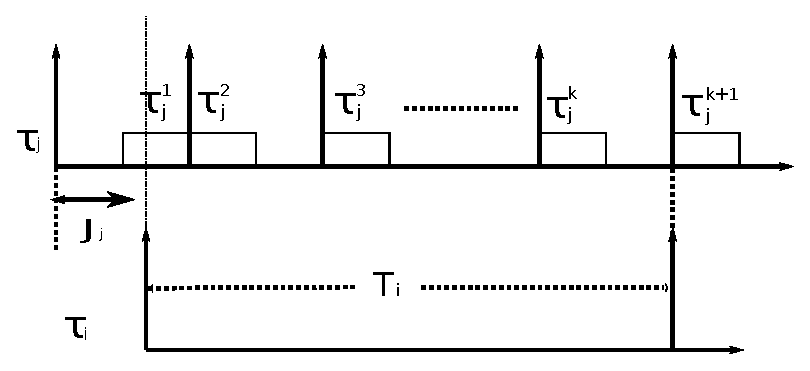
\includegraphics[bb=0bp 0bp 542bp 162bp,scale=0.5]{figures/figure9-a}
\caption{\label{fig1} Maximum interference between two tasks under G-EDF}
\end{figure}


\begin{figure}
\centering
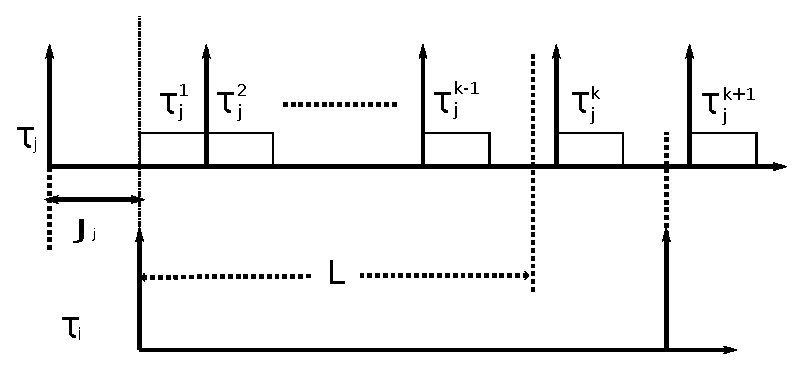
\includegraphics[bb=0bp 0bp 542bp 162bp,scale=0.5]{figures/figure9-b}
\caption{\label{fig2}Maximum interference during part $L$ of $t(T_{i})$}
\end{figure}



\subsection{Retry Cost of Atomic Sections}

\begin{figure*}
\centering
\subfigure[Early validation]{
            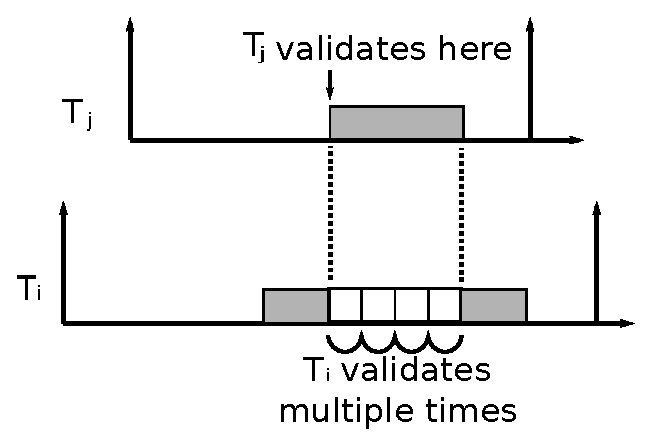
\includegraphics[scale=.45]{figures/figure5-a}
\label{fig5-a} 
}\hspace{1.2cm}
\subfigure[Lazy validation with $s_{i}^{k}(\theta)\le s_{j}^{l}(\theta)$]{
            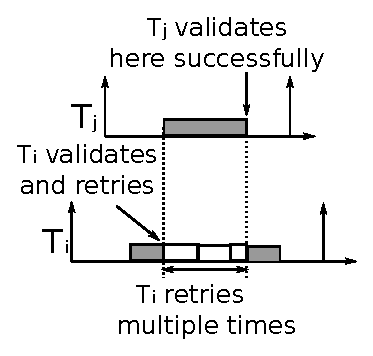
\includegraphics[scale=.65]{figures/figure5-b-1}
\label{fig5-b} 
}\hspace{1.5cm}
\subfigure[Lazy validation with $s_{i}^{k}(\theta)>s_{j}^{l}(\theta)$]{
            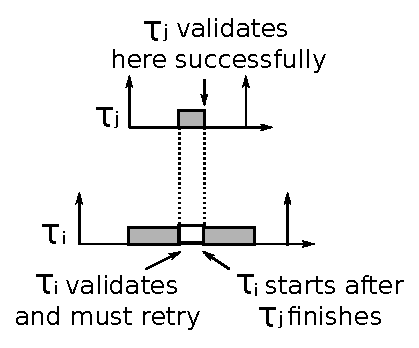
\includegraphics[scale=.65]{figures/figure5-c-1}
\label{fig5-c} 
}
\caption{Retry of $s_i^k(\theta)$ due to $s_j^l(\theta)$}  
\label{fig5}
\end{figure*}

\begin{clm}\label{gedf-edf}
Under ECM, a task $T_i$'s maximum retry cost during $t(T_i)$ is upper bounded by:
\begin{eqnarray}
RC\left(T_{i}\right) & \le & \sum_{\theta\in\theta_{i}}\Big(\Big(\sum_{T_{j}\in\gamma(\theta)}\Big(\left\lceil\frac{t\left(T_{i}\right)}{t\left(T_{j}\right)}\right\rceil\sum_{\forall s_{j}^{l}(\theta)}len\big(s_{j}^{l}(\theta)\nonumber \\
 & + & s_{max}(\theta)\big)\Big)\Big)-s_{max}(\theta)+s_{i_{max}}(\theta)\Big)\label{eq3}\end{eqnarray}
\end{clm}
\begin{proof}\normalfont
Given two tasks $T_{i}$ and $T_{j}$, where $T_{i}$ has a longer absolute deadline than $T_{j}$. When a shared object conflict occurs, the EDF CM will commit $T_{j}$ and abort and retry $T_{i}$.
Thus, an atomic section of $T_{i}$, $s_{i}^{k}(\theta)$,
will experience its maximum delay when it is at its end of the atomic section, 
%%BR: You can say "...when it is at its end," CORRECT? Since you are referring to the same section. 
and the conflicting atomic section of $T_{j}$, $s_{j}^{l}(\theta)$, starts. 
The CM will retry $s_{i}^{k}(\theta)$. 

Validation (i.e., conflict detection) in STM is usually done in two ways~\cite{austenmc:tcc:dissertation:2009}: a) eager (pessimistic), in which conflicts are detected at access time, b) lazy (optimistic), in which conflicts are detected at commit time. Despite the validation time incurred (either eager or lazy),  
$s_{i}^{k}(\theta)$ will retry for the same time duration, which is $len(s_{j}^{l}(\theta)+s_i^k(\theta))$. Then, $s_i^k(\theta)$ can commit successfully  
unless interferred by another conflicting atomic section, as shown in Figure~\ref{fig5}. 

In Figure~\ref{fig5-a}, $s_{j}^{l}(\theta)$
validates at its beginning, due to early validation, and a conflict
is detected. So $T_{i}$ retries multiple times (because at the start of each retry, $T_{i}$ validates) 
during the execution of $s_{j}^{l}(\theta)$.
When $T_{j}$ finishes its atomic section, $T_{i}$ executes its atomic section. 

In Figure~\ref{fig5-b}, 
$T_{i}$ validates at its end (due to lazy validation), and detects a conflict with $T_{j}$.
Thus, it retries, and because its atomic section length is shorter
than that of $T_{j}$, it validates again within the execution
interval of $s_{j}^{l}(\theta)$. However, the EDF CM retries it again.
This process continues until $T_{j}$ finishes its atomic section.
If $T_{i}$'s atomic section length is longer than that of $T_{j}$'s,
$T_{i}$ would have incurred the same retry time, because
$T_{j}$ will validate when $T_{i}$ is retrying, and $T_{i}$ will
retry again, as shown in Figure~\ref{fig5-c}. Thus, the retry cost
of $s_{i}^{k}(\theta)$ is $len(s_{i}^{k}(\theta)+s_{j}^{l}(\theta))$.

If multiple tasks interfere with $T_{i}$ or
interfere with each other and $T_{i}$ (see the two interference examples in Figure~\ref{fig6}), then, in each case, each atomic section of the shorter deadline tasks contributes to the delay of $s_{i}^{p}(\theta)$ by its total length, plus a retry to some atomic section in the longer deadline tasks. For example,
$s_{j}^{l}(\theta)$ contributes by $len(s_{j}^{l}(\theta)+s_{i}^{p}(\theta))$
in both figures~\ref{fig6-a} and~\ref{fig6-b}. 
%%BR: YOu should say "..in both Figures~\ref{fig6-a} and~\ref{fig6-b}."
In Figure~\ref{fig6-b}, $s_{k}^{y}(\theta)$ causes a retry 
to $s_{j}^{l}(\theta)$, and $s_{h}^{w}(\theta)$ causes a retry to $s_{k}^{y}(\theta)$.


Since we do not know in advance which atomic section will be retried
due to another, we can safely assume that, each atomic section (that share the same object with  $T_i$) in a shorter deadline task contributes by its total length, in addition to the maximum length between all atomic sections that share the same object, $len(s_{max}(\theta))$. Thus, 
\begin{equation}
\mbox{\ensuremath{W_{i}^{p}\left(s_{j}^{k}\left(\theta\right)\right)\le len\left(s_{j}^{k}\left(\theta\right)+s_{max}\left(\theta\right)\right)}}\label{eq2}\end{equation}


Thus, the total contribution of all atomic sections of all other tasks
that share objects with a task $T_i$ 
to the retry cost of $T_i$ during $T_i$'s period $t(T_{i})$ is:
\begin{eqnarray}
RC\left(T_{i}\right) & \le & \sum_{\theta\in\theta_{i}}\sum_{T_{j}\in\gamma(\theta)}\Big(\left\lceil\frac{t\left(T_{i}\right)}{t\left(T_{j}\right)}\right\rceil\sum_{\forall s_{j}^{l}(\theta)}len\big(s_{j}^{l}(\theta)\nonumber \\
 & + & s_{max}(\theta)\big)\Big)\label{eq3-1}\end{eqnarray}



Here, $\left\lceil\frac{t\left(T_{i}\right)}{t\left(T_{j}\right)}\right\rceil\sum_{\forall s_{j}^{l}\left(\theta\right)}len\left(s_{j}^{l}\left(\theta\right)+s_{max}\left(\theta\right)\right)$ is  the contribution of all instances of $T_{j}$ during $t(T_{i})$. This contribution is added to all tasks. The last atomic section to execute is $s_{i}^{p}(\theta)$ ($T_i$'s atomic section that was delayed by conflicting atomic sections of other tasks). One of the other atomic sections (e.g., $s_{m}^{n}(\theta)$) should have a contribution $len(s_{m}^{n}(\theta)+s_{i_{max}}(\theta))$, instead of $len(s_{m}^{n}(\theta)+s_{max}(\theta))$. That is why one $s_{max}(\theta)$ should be subtracted, and $s_{i_{max}}(\theta)$ should be added (i.e., $s_{i_{max}}(\theta)-s_{max}(\theta)$). Claim follows.
\end{proof}

\begin{figure*}%[htbp]%
\centering%
\subfigure[Other atomic sections interfere only with $s_i^p(\theta)$]{
            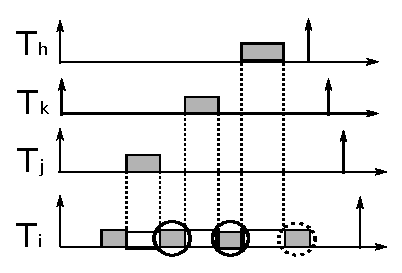
\includegraphics[scale=.65]{figures/figure6-a-1}
\label{fig6-a} 
}\hspace{1cm}
\subfigure[All atomic sections interfere with each other and $s_i^p(\theta)$]{
            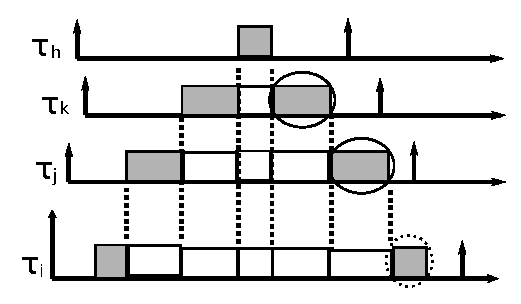
\includegraphics[scale=.6]{figures/figure6-b}
\label{fig6-b} 
}
\begin{tabular}{>{\centering}p{1cm}l}
\includegraphics[scale=0.45]{figures/circle} & Replaced in calculations by $s_{max}(\theta)$\tabularnewline
\includegraphics[scale=0.45]{figures/dotted_circle} & Replaced in calculations by $s_{i_{max}}(\theta)$\tabularnewline
\end{tabular}
\caption{Retry of $s_i^p(\theta)$ due to other atomic sections}  
\label{fig6}
\end{figure*}

\begin{clm}
Claim~\ref{gedf-edf}'s retry bound can be minimized as:
\begin{equation}
RC(T_{i})\le \sum_{\theta\in\theta_{i}}min(\Phi_1 , \Phi_2)\label{eq5}\end{equation}
where $\Phi_1$ is calculated by (\ref{eq3}) for one object $\theta$ (not the sum of $\theta \in \theta_i$),  and 
\begin{eqnarray}
\Phi_2 & = & \Big(\sum_{T_{j}\in\gamma(\theta)} \Big(\left\lceil\frac{t\left(T_{i}\right)}{t\left(T_{j}\right)}\right\rceil\sum_{\forall s_{j}^{l}(\theta)}len \big(s_{j}^{l}(\theta)\nonumber \\
 &  & +s_{max}^{*}(\theta) \big) \Big) \Big)-\bar{s}_{max}(\theta)+s_{i_{max}}(\theta)\label{eq4}\end{eqnarray}
\end{clm}
\begin{proof}\normalfont
(\ref{eq3}) can be modified by noting that a task $T_i$'s atomic section 
may conflict with those of other tasks, but not with $T_i$. 
This is because, tasks are assumed to arrive sporadically, and  each instance finishes before the next begins. 
Thus, (\ref{eq3}) becomes:
\begin{eqnarray}
RC(T_{i}) & \le & \sum_{\forall\theta\in\theta_{i}} \Big( \Big(\sum_{T_{j}\in\gamma(\theta)} \Big(\left\lceil\frac{t\left(T_{i}\right)}{t\left(T_{j}\right)}\right\rceil\sum_{\forall s_{j}^{l}(\theta)}len \big(s_{j}^{l}(\theta)\nonumber \\
 &  & +s_{max}^{*}(\theta) \big) \Big) \Big)-\bar{s}_{max}(\theta)+s_{i_{max}}(\theta) \Big)\label{eq4-1}\end{eqnarray}
where, $s_{max}^{*}(\theta)\in s(\theta)$ and $s_{max}^{*}(\theta)\not\in s_{j}(\theta)$, 
because $T_{j}$ will not cause a retry to one of its instances.


To obtain $\bar{s}{}_{max}(\theta)$, the maximum-length atomic section of each task that accesses $\theta$ is grouped into an array, in non-increasing order of their lengths. $s_{max}(\theta)$ will be the first element of this array, and $\bar{s}_{max}(\theta)$ will be the next element, as illustrated in Figure~\ref{fig7}, where the maximum atomic
section of each task that accesses $\theta$ is associated with
its corresponding task. In (\ref{eq4-1}), all tasks
but $T_{j}$ will choose $s_{j_{max}}(\theta)$ as the value of $s_{max}^{*}(\theta)$,
as it is the maximum-length atomic section not associated with the interfering task. 
But when $T_{j}$ is the one whose contribution is studied,
it will choose $s_{k_{max}}(\theta)$, as it is the maximum one not
associated with $T_{j}$. This way, it can be seen that the maximum
value always lies between the two values $s_{jmax}(\theta)$ and $s_{kmax}(\theta)$. 
Of course, these two values can be equal, or the maximum value can be associated with $T_i$ itself, and not with any one of the interfering tasks. In the latter case,
the chosen value will always be the one associated with $T_i$, and yet, it will lie between the two largest values. 

\begin{figure}[htbp]
\centering
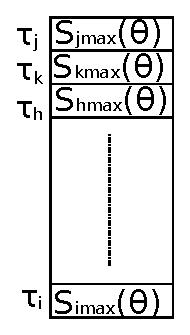
\includegraphics[scale=0.7]{figures/figure7}
\caption{\label{fig7}Values associated with $s_{max}^{*}(\theta)$}
\end{figure}


This means that the subtracted $s_{max}(\theta)$ in (\ref{eq3})
must be replaced with one of these two values ($s_{max}(\theta)$ or $\bar{s}_{max}(\theta)$). However, since we do not know  which task will interfere with $T_i$, the minimum is chosen, as we are determining the worst case retry cost (as this value is going to be subtracted),
and this minimum is the second maximum.


Let $p_j = \left\lceil{\frac{t(T_{i})}{t(T_{j})}}\right\rceil$,
$g_j$ be the number of times $T_j$ accesses $\theta$,  
and 
$Const_j = \left\lceil{\frac{t(T_{i})}{t(T_{j})}}\right\rceil \times \sum_{\forall{s_{j}^{l}(\theta)}}{len(s_{j}^{l}(\theta))}$. 
If $\theta_1$'s maximum-length atomic section is associated with $T_i$ (i.e., $s_{max}(\theta_1)=s_{i_{max}}(\theta_1)$), all other tasks will choose it, and $\Phi_1$ (the result of (\ref{eq3}) for $\theta_1$) will be 
$\sum_{\forall {T_j \in \gamma(\theta_1)}} \left(Const_j +p_j g_j s_{i_{max}}(\theta_1)\right)-s_{i_{max}}(\theta_1)+s_{i_{max}}(\theta_1)$,
whereas $\Phi_2$ (the result of (\ref{eq4-1}) for $\theta_1$) will be $\sum_{\forall {T_j \in \gamma(\theta_1)}} \left(Const_j+ p_j g_j s_{i_{max}}(\theta_1)\right)-s_{k_{max}}(\theta_1)+s_{i_{max}}(\theta_1)$. 
Since $s_{k_{max}}(\theta_1)\leq s_{i_{max}}(\theta_1)$, $\Phi_1 \le \Phi_2$.


Let the maximum-length atomic section for $\theta_2$ be $s_{d_{max}}(\theta_2)$  
($s_{max}(\theta_2)=s_{d_{max}}(\theta_2)$), 
and be associated with another task $T_{d}$, and not with $T_{i}$. Let $ s_{k_{max}}(\theta_2) = \bar{s}_{max}(\theta_2)$,  which will be the second minimum. 
Let $T_{d}$ has $g_d$ atomic sections that share $\theta_2$ with $T_i$. Then, $\Phi_1$ 
for $\theta_2$ will result in $\sum_{\forall T_j \in \gamma(\theta_2)} \left(Const_j +p_j g_j s_{d_{max}}(\theta_2)\right) -s_{d_{max}}(\theta_2)+s_{i_{max}}(\theta_2)$,
and $\Phi_2$ will be $\sum_{\forall T_j \in \gamma(\theta_2) \wedge T_j \ne T_d} \left(Const_j+ p_j g_j s_{d_{max}}(\theta_2)\right)+ Const_d+p_d g_d s_{k_{max}}(\theta_2) -s_{k_{max}}(\theta_2)+s_{i_{max}}(\theta_2)$. So, $\Phi_1 - \Phi_2 =(p_d g_d -1)(s_{d_{max}}(\theta_2)-s_{k_{max}}(\theta_2))$. Since $T_d$ has at least one job that shares $\theta_2$ with $T_i$ (otherwise, $T_d$ would not be included in $\gamma (\theta_2)$), $p_d g_d -1 \ge 0$. Since $s_{d_{max}}(\theta_2) \ge s_{k_{max}}(\theta_2)$, $\Phi_1 \ge \Phi_2$. 


Thus, given an object $\theta$, $\Phi_1$ may be greater, smaller, or equal to $\Phi_2$. The minimum of $\Phi_1$ and $\Phi_2$ therefore yields the worst-case contribution for $\theta$ in $RC(T_i)$. Claim follows.
\end{proof}


\subsection{Upper Bound on Response Time}

To obtain an upper bound on the response time of a task $T_{i}$, the term $RC(T_{i})$ must be added to the workload of other tasks during the non-atomic
execution of $T_{i}$. But this requires modification of the WCET of each
task as follows. 
%starthere
The WCET, $c_{j}$, of each interfering task $T_{j}$ should be inflated to accommodate for the interference of tasks other than $T_{k},$ $k\ne j,i$. Meanwhile, atomic regions that access shared objects between $T_{j}$ and $T_{i}$ should not be considered in the inflation cost, because they have already been calculated in $T_{i}$'s retry cost. Thus, $T_{j}$'s inflated WCET becomes:
\begin{equation}
c_{ji}=c_{j}-\left(\sum_{\theta\in(\theta_{j}\wedge\theta_{i})}len \left(s_{j}(\theta) \right) \right)+RC(T_{ji})\label{eq9}\end{equation}
where, $c_{ji}$ is the new WCET of $T_{j}$ relative to $T_{i}$; 
the sum of lengths of all atomic sections in $T_{j}$ that access object $\theta$ is $\sum_{\theta \in (\theta_j \wedge \theta_i)} {len(s_{j}(\theta))}$; and $RC(T_{ji})$ is the $RC(T_j)$ 
 without including the shared objects between $T_{i}$ and $T_{j}$.
The calculated WCET is relative to task $T_{i}$, as it changes from task to task. The upper bound on the response time of $T_{i}$, denoted $R_{i}^{up}$, can be calculated iteratively, using a modification of Theorem 6 in~\cite{key-2}, as follows:
\begin{equation}
R_{i}^{up}=c_{i}+RC(T_{i})+\left\lfloor\frac{1}{m}\sum_{j\ne i}W_{ij}(R_{i}^{up})\right\rfloor
\label{eq10}
\end{equation}
where $R_{i}^{up}$'s initial value is $c_{i}+RC(T_{i})$.

$W_{ij}(R_{i}^{up})$ is calculated by (\ref{eq13}), and $W_{ij}^{*}(t(T_{i}))$
is calculated by (\ref{eq11}), with $c_{j}$ replaced by 
$c_{ji}$, and changing $\hat{W}_{ij}(L)$ as:
\begin{equation}
\hat{W}_{ij}(L(T_{i}))=max\begin{cases}
\left(\left\lceil\frac{L-c_{ji}-\sum_{\theta\in(\theta_{j}\wedge\theta_{i})}len(s_{j}(\theta))}{t(T_{j})}\right\rceil+1 \right).c_{ji}\\
\left\lceil\frac{L-c_{j}}{t(T_{j})}\right\rceil.c_{ji}+c_{j}-\sum_{\theta\in(\theta_{j}\wedge\theta_{i})}len(s_{j}(\theta))\end{cases}\label{eq14}\end{equation}

(\ref{eq14}) compares between two terms, as we have two cases:


\textit{Case 1}. The carried-in job (i.e., a job whose release is before $r(T_i)$ and its deadline is after $r(T_i)$ but before $d(T_i)$, as defined in~\cite{key-2}) of $T_j$
contributes by $c_{ji}$. Thus, other instances of $T_j$ will begin after this modified WCET, but the sum of the shared objects' atomic section lengths is removed from $c_{ji}$, causing other instances to start earlier. Thus, the term $\sum_{\theta\in(\theta_i\wedge\theta_j)} {len(s_{j}(\theta))}$ is added to $c_{ji}$ to obtain the correct start time. 

\textit{Case 2}. $T_j$'s carried-in job contributes its $c_j$. Thus, other instances begin after this $c_j$ of the carried-in job (as shown in Figure~\ref{fig2}), but the sum of the shared atomic section lengths  between $T_i$ and $T_j$ should be subtracted from this carried-in
instance, as they are already included in the retry cost. 

It should be noted that subtraction of the sum of the shared objects' atomic section lengths is done in the first case to obtain the correct start time of other instances, while in the second case, this is done to get the correct contribution of the carried-in  instance. The maximum is chosen from the two terms in (\ref{eq14}), because they differ in the contribution of their carried-in jobs, and the number of instances after that.

\subsubsection{Tighter Upper Bound}

To tighten $T_{i}$'s response time upper bound, the response time can be calculated recursively over duration $R_i^{up}$, 
and not directly over $t(T_i)$, as done in (\ref{eq10}). Thus, $RC(T_{i})$ will change according
to $T_i$'s recursive response time (i.e., $R_{i}^{up}$). So, (\ref{eq5}) must be changed to include the modified number of interfering instances, in the same way this term  
is calculated in (\ref{eq13}). Also, when calculating this term 
for the entire $t(T_{i})$, a situation like that shown in Figure
\ref{fig10} can happen.
\begin{figure}
\centering{}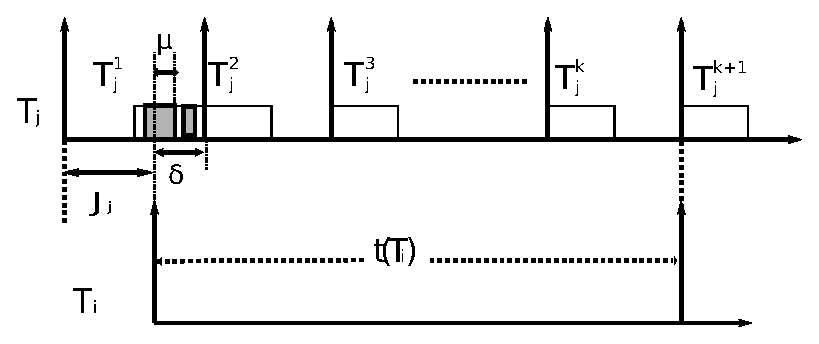
\includegraphics[scale=0.5]{figures/figure10}\caption{\label{fig10} Atomic sections of job $T_{j}^{1}$ contributing to period $t(T_i)$}
\end{figure}


Atomic sections of $T_{j}^{1}$ that are contained in the interval $\delta$
are the only ones that can contribute to $RC(T_{i})$. Of course, they can be lower, but cannot be greater, because $T_{j}^{1}$ has been delayed by its maximum jitter. Hence, no more atomic sections
can interfere during the duration 
$[d(T_{j}^{1})-\delta,d(T_{j}^{1})]$. Even though only one of $T_j^1$'s atomic sections contributes by length $\mu$ to $T_i$, the effect of this $\mu$ will still be the retry of one of the other atomic sections. 

For simplicity, we use the following notations:
\begin{compactitem}
\item $\lambda_{1}\left(j,\theta\right)=\sum_{\forall s_{j}^{l}\left(\theta\right)\in\left[d\left(T_{j}^{1}\right)-\delta,d\left(T_{j}^{1}\right)\right]^{*}}len\left(s_{j}^{l^{*}}\left(\theta\right)+s_{max}\left(\theta\right)\right)$
\item $\chi_{1}\left(i,j,\theta\right)=\left\lfloor\frac{t\left(T_{i}\right)}{t\left(T_{j}\right)}\right\rfloor\sum_{\forall s_{j}^{l}\left(\theta\right)}len\left(s_{j}^{l}\left(\theta\right)+s_{max}\left(\theta\right)\right)$
\item $\lambda_{2}\left(j,\theta\right)=\sum_{\forall s_{j}^{l}\left(\theta\right)\in\left[d\left(T_{j}^{1}\right)-\delta,d\left(T_{j}^{1}\right)\right]^{*}}len\left(s_{j}^{l^{*}}\left(\theta\right)+s_{max}^{*}\left(\theta\right)\right)$
\item $\chi_{2}\left(i,j,\theta\right)=\left\lceil\frac{t\left(T_{i}\right)}{t\left(T_{j}\right)}\right\rceil\sum_{\forall s_{j}^{l}\left(\theta\right)}len\left(s_{j}^{l}\left(\theta\right)+s_{max}^{*}\left(\theta\right)\right)$
\end{compactitem}
Here, $s_{j}^{l^{*}}\left(\theta\right)$ is the part of $s_{j}^{l}\left(\theta\right)$ that
is included in interval $\delta$. The term $\left[d\left(T_{j}^{1}\right)-\delta,d\left(T_{j}^{1}\right)\right]^{*}$ contains $s_{j}^{l}\left(\theta\right)$, whether it is partially or totally included in it. If it is partially included, $s_{j}^{l}(\theta)$
will contribute by its included length $\mu$.

Now, (\ref{eq5}) can be modified as:
\begin{equation}
RC_{}\left(t\left(T_{i}\right)\right)\le \sum_{\theta\in\theta_{i}}min\begin{cases}
\begin{cases}
\Bigl(\left(\sum_{T_{j}\in\gamma\left(\theta\right)}\lambda_{1}\left(j,\theta\right)+\chi_{1}\left(i,j,\theta\right)\right)\\
-s_{max}\left(\theta\right)+s_{i_{max}}\left(\theta\right)\Bigr)\end{cases}\\
\begin{cases}
\Bigl(\left(\sum_{T_{j}\in\gamma\left(\theta\right)}\lambda_{2}\left(j,\theta\right)+\chi_{2}\left(i,j,\theta\right)\right)\\
-\bar{s}_{max}\left(\theta\right)+s_{i_{max}}\left(\theta\right)\Bigr)\end{cases}\end{cases}\label{eq15}\end{equation}



We can compute $RC\left(T_{i}\right)$ during a duration of length $L$, which does not extend to the last instance of $T_{j}$. Let:
\begin{compactitem}
\item $\upsilon\left(L,j\right)=\left\lceil\frac{L-c_{j}}{t\left(T_{j}\right)}\right\rceil+1$
\item $\lambda_{3}\left(j,\theta\right)=\sum_{\forall s_{j}^{l}\left(\theta\right)}len\left(s_{j}^{l}\left(\theta\right)+s_{max}\left(\theta\right)\right)$
\item $\lambda_{4}\left(j,\theta\right)=\sum_{\forall s_{j}^{l}\left(\theta\right)}len\left(s_{j}^{l}\left(\theta\right)+s_{max}^{*}\left(\theta\right)\right)$
\end{compactitem}
Now, (\ref{eq5}) becomes: 
\begin{equation}
RC\left(L\left(T_{i}\right)\right)\le \sum_{\theta\in\theta_{i}}min\begin{cases}
\begin{cases}
\left(\sum_{T_{j}\in\gamma\left(\theta\right)}\left(\upsilon\left(L,j\right)\lambda_{3}\left(j,\theta\right)\right)\right)\\
-s_{max}\left(\theta\right)+s_{i_{max}}\left(\theta\right)\end{cases}\\
\begin{cases}
\left(\sum_{T_{j}\in\gamma\left(\theta\right)}\left(\upsilon\left(L,j\right)\lambda_{4}\left(j,\theta\right)\right)\right)\\
-\bar{s}_{max}\left(\theta\right)+s_{i_{max}}\left(\theta\right)\end{cases}\end{cases}\label{eq16}\end{equation}


Thus, an upper bound on $RC(T_i)$ is given by:
\begin{equation}
RC(R_{i}^{up})\le min\begin{cases}
RC(R_{i}^{up}(T_{i}))\\
RC(t(T_{i}))\end{cases}
\label{eq17}
\end{equation}

The final upper bound on $T_{i}$'s response time can be calculated
as in (\ref{eq10}) by replacing $RC(T_{i})$ with
$RC(R_{i}^{up})$.

\section{G-RMA/RMA CM Response Time}
\label{sec:g-rma-rma-cm}

As G-RMA is a fixed priority scheduler,  a task $T_{i}$ will be interfered by those tasks with priorities higher than $T_{i}$ (i.e., $p(T_{j}) > p(T_{i})$).  Upon a conflict, the RMA CM will commit the transaction that belongs to the higher priority task. We will use \emph{RCM} to refer to a multiprocessor system scheduled by G-RMA and resolves STM conflicts by the RMA CM.


\subsection{Maximum Task Interference}


Figure~\ref{fig11} illustrates the maximum interference caused by a task $T_{j}$
to a task $T_{i}$ under G-RMA. As $T_{j}$ is of higher priority than $T_{i}$,
$T_{j}^{k}$ will interfere with $T_{i}$ even if it is not totally
included in $t(T_{i})$. Unlike the G-EDF case shown in Figure~\ref{fig10}, 
where only the $\delta$ part of $T_{j}^{1}$ is considered, in G-RMA,
$T_{j}^{k}$ can contribute by the whole $c_{j}$, and all atomic
sections contained in $T_{j}^{k}$ must be considered. This is because, in G-EDF, the worst-case pattern releases $T_{i}$ before $d(T_{j}^{1})$
by $\delta$ time units, and $T_{i}$ cannot be interfered before it
is released. But in G-RMA, $T_{i}$ is already released, and can be
interfered by the whole $T_{j}^{k}$, even if this makes it infeasible.


\begin{figure}[htbp]
\centering
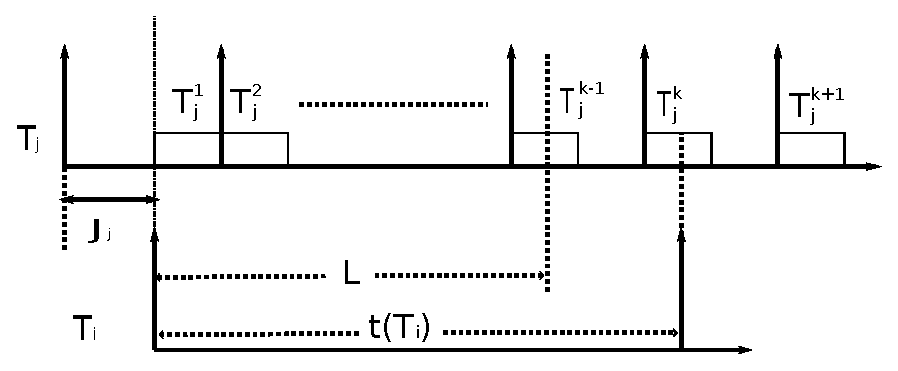
\includegraphics[scale=0.5]{figures/figure11}\caption{\label{fig11}Max interference of $T_{j}$ to $T_{i}$ in G-RMA}
\end{figure}

Thus, the maximum contribution of $T_{j}$ to $T_{i}$ for any duration
$L$ can be deduced from Figure~\ref{fig11} as $W_{ij}(L(T_{i}))=\left(\left\lceil\frac{L-c_{j}}{t(T_{j})}\right\rceil+1 \right).c_{j}$,
where $L$ can extend to $t(T_{i})$. In contrast to ECM where $L$ cannot be extended directly to $t(T_i)$, as this will have a different pattern of worst case interference from other tasks.

\subsection{Retry Cost of Atomic Sections}

\begin{clm}
Under RCM, a task $T_i$'s retry cost over duration $L(T_i)$, which can extend to $t(T_i)$, is upper bounded by:
\begin{eqnarray}
RC\left(L\left(T_{i}\right)\right) & \le & \sum_{\theta\in\theta_{i}}\Bigg(\left(\sum_{T_{j}^{*}}\left(\left(\left\lceil\frac{L-c_{j}}{t\left(T_{j}\right)}\right\rceil+1\right)\pi\left(j,\theta\right)\right)\right)\nonumber \\
 & - & s_{max}^{j}\left(\theta\right)+s_{i_{max}}\left(\theta\right)\Bigg)\label{eq20}\end{eqnarray}
 where:
 \begin{compactitem}
\item $T_{j}^{*}=\{T_{j}|(T_{j}\in\gamma(\theta))\wedge(p(T_{j})> p(T_{i})\}$
\item $\pi(j,\theta)=\sum_{\forall s_{j}^{l}(\theta)}len\left(s_{j}^{l}\left(\theta\right)+s_{max}^{j}\left(\theta\right)\right)$
\end{compactitem}
\end{clm}
\begin{proof}\normalfont
Since the worst case interference pattern for RCM is the same as that for ECM for an interval $L$, except that, in RCM, $L$ can extend to the entire duration of $t(T_i)$, but in ECM, it cannot, as the interference pattern of $T_j$ to $T_i$ changes. 
So, (\ref{eq16}) can be used to calculate $T_i$'s retry cost, with some modifications, as we do not have to obtain the minimum of the two terms in (\ref{eq16}), because $T_j$'s atomic sections will abort and retry only atomic sections of tasks with lower priority than $T_j$. Thus, $s_{max}(\theta)$, $s_{max}^*(\theta)$, and $\bar{s}_{max}(\theta)$ are replaced by $s_{max}^j(\theta)$, which is the maximum-length atomic section of tasks with priority lower than $T_j$ and share object $\theta$ with $T_i$. Besides, as $T_i$'s atomic sections can be aborted only by atomic sections of higher priority tasks, not all $T_j \in \gamma (\theta)$ are considered, but only the subset of tasks in $\gamma (\theta)$ with priority higher than $T_i$ (i.e., $T_j^*$). 
%Claim follows.
\end{proof}



\subsection{Upper Bound on Response Time}

The response time upper bound can be computed by Theorem 7 in~\cite{key-2} with some modification to include the effect of retry cost. Thus, this upper bound is given by:
\begin{equation}
R_{i}^{up}=c_{i}+RC(R_{i}^{up})+\left\lfloor\frac{1}{m}\sum_{j\ne i}\hat{W}{}_{ij}(R_{i}^{up})\right\rfloor\label{eq22}\end{equation}
where $\hat{W}_{ij}(R_{i}^{up})$ is calculated as in (\ref{eq14}), $c_{ji}$ is calculated by (\ref{eq9}), and $RC$ is calculated by (\ref{eq20}).


\section{FMLP and OMLP Blocking Times}
\label{sec:blocking-bound-fmlp-omlp}

A number of protocols have been proposed for synchronization in real-time systems as shown in Table~\ref{table 2}. The FMLP protocol~\cite{brandenburg2008comparison} has been shown to be superior to other multiprocessor real-time locking protocols in terms of schedulability, and the global OMLP protocol~\cite{key-3} has been shown to be asymptotically optimal. To formally compare STM against FMLP and global OMLP, we first upper bound their blocking times. %(those were not presented in~\cite{brandenburg2008comparison,key-4,key-3}). 
\begin{table*}
\caption{\label{table 2}Some synchronization protocols }
\begin{adjustwidth}{-2.5cm}{}
\begin{tabular}{|>{\centering}m{4cm}|>{\centering}m{2cm}|c|c|c|c|c|>{\centering}m{1cm}|}
\hline 
 &  & \multicolumn{6}{>{\centering}m{1.5cm}|}{{\small Multiprocessor}}\tabularnewline
\cline{3-8} 
{\small Protocol} & {\small Uniprocessor} & \multicolumn{3}{c|}{{\small Global}} & \multicolumn{3}{>{\centering}m{1.5cm}|}{{\small Partitioned}}\tabularnewline
\cline{3-8} 
 &  & {\small G-EDF} & {\small PFair} & {\small Others} & {\small P-EDF} & {\small Static Priority} & {\small Others}\tabularnewline
\hline 
{\small PCP\cite{chen1990dynamic}} & {\small $\checkmark$} &  &  &  &  &  & \tabularnewline
\hline 
{\small SRP\cite{baker1991stack}} & {\small $\checkmark$} &  &  &  &  &  & \tabularnewline
\hline 
{\small PCP variant\cite{Rajkumar:1991:SRS:532621}} &  &  &  &  &  & {\small $\checkmark$} & \tabularnewline
\hline 
{\small PCP variant\cite{sha1990priority}} &  &  &  &  &  & {\small $\checkmark$} & \tabularnewline
\hline 
{\small MPCP\cite{lakshmanan2009coordinated,rajkumar2002real}} &  &  &  &  &  & {\small $\checkmark$} & \tabularnewline
\hline 
{\small DPCP\cite{rajkumar2002real}} &  &  &  &  &  & {\small $\checkmark$} & \tabularnewline
\hline 
{\small \cite{chen1998multiprocessor}} &  &  &  &  & {\small $\checkmark$} &  & \tabularnewline
\hline 
{\small SRP implementation\cite{lopez2004utilization}} &  &  &  &  & {\small $\checkmark$} &  & \tabularnewline
\hline 
{\small SRP implementation\cite{gai2003comparison}} &  &  &  &  & {\small $\checkmark$} &  & \tabularnewline
\hline 
{\small \cite{holman2006locking}} &  &  & {\small $\checkmark$} &  &  &  & \tabularnewline
\hline 
{\small PPCP\cite{easwaran2009resource}} &  &  &  & {\small $\checkmark$} &  &  & \tabularnewline
\hline 
{\small PIP\cite{easwaran2009resource}} &  &  &  &  &  &  & \tabularnewline
\hline 
{\small \cite{key-5}} &  & {\small $\checkmark$} &  &  &  &  & \tabularnewline
\hline 
{\small FMLP\cite{key-4,brandenburg2008implementation}} &  & {\small $\checkmark$(GSN-EDF)} & {\small $\checkmark$} &  & {\small $\checkmark$(PSN-EDF)} & {\small $\checkmark$} & \tabularnewline
\hline 
{\small OMLP\cite{key-3}} &  & {\small $\checkmark$} &  & {\small $\checkmark$JLSP} & {\small $\checkmark$} &  & \centering{}{\small $\checkmark$JLSP}\tabularnewline
\hline
\end{tabular}
\end{adjustwidth}
\end{table*}


\subsection{\label{global-fmlp}Global FMLP}

FMLP can be used with global and partitioned scheduling. Since we only consider global scheduling, ``FMLP" and ``global FMLP" mean the same, for the paper's purpose.


FMLP divides shared objects into short resources, $s\_\theta$, and long ones, $l\_\theta$. Nested resources 
are grouped together into two groups: $g(s\_\theta)$ that contains only short resources, and $g(l\_\theta)$ that contains only long resources.
A request $R_i (g(s\_\theta))$ is made by a task $T_i$ to access one or more resources in $g(s\_\theta)$. This request's length is denoted $|R_i (g(s\_\theta))|$, and the number of times $T_i$ requests short resources is denoted $N_{i,s}$. Similarly, $R_i (g(l\_\theta))$ is $T_i$'s request to a group containing long resources for a duration $|R_i (g(l\_\theta))|$, and $N_{i,l}$ is the number of times $T_i$ requests long resources.


Global FMLP uses a variant of G-EDF (called GSN-EDF which discriminates between
linked jobs and scheduled ones) to account for non-preemptive jobs while still using G-EDF for scheduling, 
%%BR: "jobs"?? (can there be multiple linked jobs)?
%%BR: "ones"?? (can there be multiple scheduled ones)?
Tasks busy-wait on short resources, and suspend on long ones. In both cases, requests for resources are arranged in FIFO queues, 
%%BR: "FIFO queue" or "FIFO queues"???? (since there are two resource types)
and for requesting long resources, the task holding the resource inherits the highest priority of the suspended tasks on that resource. For short resources, there is no need to inherit priorities, as tasks become non-preemptable when acquiring short resources. 

Requests for long resources can contain requests for the short resource group, but the reverse is not true. The protocol allows non-preemptable jobs and bounds the time a job is non-preemptively blocked by a lower priority job as the maximum time a non-preemptive section of the job can be linked to the processor of the higher priority job. This non-preemptive blocking can only happen when the higher priority job is released or resumed.


Three types of blocking can be incurred by any task under global FMLP. These include busy-wait blocking, non-preemptive blocking, and direct blocking. The total blocking time of a job, $b_{i}$, is the sum of these three blocking durations. Execution time of each task, $e_{i}$, is inflated by this blocking amount ($e_{i}+b_{i}$), and is used in any of the G-EDF schedulability tests (e.g.,~\cite{Goossens:2003:PSP:876600.876615,srinivasan2002deadline}) 
for verifying schedulability. 

We upper bound a task's blocking durations due to busy-wait blocking, non-preemptive blocking, and direct blocking, denoted as $BW(T_{i})$, $NPB(T_{i})$, and $DB(T_{i})$, respectively, as follows.  
(Note that, in~\cite{key-3}, no upper bounds are presented for these terms, except for $DB(T_{i})$, as~\cite{key-3}'s main focus is on FMLP's suspension-based part. Also, the upper bound for $DB(T_{i})$ in~\cite{key-3} does not consider the effect of requesting a short resource within a long one.)


A job $T_{i}^{j}$ busy-waits in a FIFO queue when it is scheduled on a processor and it cannot be removed by any other task until its request is satisfied. As busy-waiting tasks are non-preemptable, job $T_{i}^{j}$ can be blocked for at most the maximum $m-1$ requests, where each request consists of the sum of the nested requests
to some resources in the same group. This process proceeds for each short resource requested by $T_{i}$. The busy-wait blocking time, $BW(T_{i})$, is therefore:
\begin{equation}
BW(T_{i})\le\sum_{s\_\theta\in\theta_{i}} \left(max \left[\sum_{k=1,k\ne i}^{min(m,n)-1} \left| R_{k} \left(g \left(s\_\theta \right) \right) \right| \right] \right)\label{eq26}
\end{equation}

A job $T_{i}^{j}$ can be non-preemptively blocked, either at its release or when it resumes, by at most the maximum (nested) request to any short resource. The non-preemptive blocking time, $NPB(T_{i})$, is therefore:
\begin{equation}
NPB(T_{i})=(1+N_{i,l}).max_{k\ne i} \left| R_{k}(g(s\_\theta)) \right|\label{eq27}
\end{equation}
Here, $1$ is added to $N_{i,l}$, because $T_{i}$ can be non-preemptively blocked at its release, in addition to suspension times. 

A job $T_{i}^{j}$ can be blocked by all other $n-1$ tasks for any long resource. Any of these $n-1$ requests can be a nested request to long resources belonging to the same group. In addition, any of those requests can contain a request to a short resource, and so it can busy-wait on it. Thus, each request in the $n-1$ requests, requiring access to a short resource, can be delayed by at most the maximum $m-1$ requests to the group containing that short resource. The direct blocking time, $DB(T_{i})$, is therefore:
\begin{equation}
DB(T_{i})\le\sum_{l\_\theta\in\theta_{i}} \left[max_{k=1,k\ne i}^{n-1} \left|R_{k} \left(g \left(l\_\theta \right) \right) \right| \right]
\label{eq28}
\end{equation}


\subsection{Global OMLP}


In~\cite{key-3}, 
global FMLP has a maximum s-oblivious pi-blocking cost of $\Theta(n)$, whereas global OMLP~\cite{key-3}, which is a suspension-based protocol that supports G-EDF, as well as any global job-level static priority (JLSP) scheduler, has a $\Theta(m)$ s-oblivious pi-blocking cost, as seen by equation (\ref{eq29}):
\begin{equation}
b_{i}\triangleq\sum_{k=1}^{q}N_{i,k}.2.(m-1).max_{1\le i\le n}\{L_{i,k}\}\label{eq29}\end{equation}
where $N_{i,k}$ is the maximum number of times $T_i$ requests resource $k$, and $L_{i,k}$ is the maximum execution time of such a request. $N_{i,k}$ and $L_{i,k}$ are assumed to be constants,
so the s-oblivious pi-blocking is $\Theta(m)$, and thus it is optimal.

\section{STM versus Locks and Lock-Free}
\label{sec:comparison}

We now would like to understand when STM will be beneficial, and when FMLP/global OMLP and lock-free approaches will be so. 
We consider the lock-free retry-loop approach for G-EDF in~\cite{key-5}, where a retry upper bound is developed by computing the worst-case number of tasks that can execute within one period of the task being considered. This lock-free approach is the most relevant to our work. 


\subsection{\label{sub:G-EDF-scheduler-with} ECM versus Lock-Free}

\begin{clm}
For ECM's schedulability to be better or equal to that of~\cite{key-5}'s retry-loop lock-free approach,  
the size of $s_{max}$ must not exceed one half of that of $r_{max}$; with low number of conflicting tasks, the size of $s_{max}$ can be at most the size of $r_{max}$. 
\end{clm}
\begin{proof}\normalfont
Equation (\ref{eq17}) can be upper bounded as:
\begin{equation}
RC\left(T_{i}\right) \le \sum_{T_{j}\in\gamma_{i}}\left(\sum_{\theta\in\theta_{i}}\left(\left\lceil\frac{t\left(T_{i}\right)}{t\left(T_{j}\right)}\right\rceil\sum_{\forall s_{j}^{l}\left(\theta\right)}\left(2.s_{max}\right)\right)\right)
\label{eq30}
\end{equation}
where $s_{j}^{l}\left(\theta\right)$, $s_{max}\left(\theta\right)$, $s_{i_{max}}\left(\theta\right)$,
$s_{max}^{*}\left(\theta\right)$, and $\bar{s}_{max}\left(\theta\right)$ are replaced by $s_{max}$, and the order of the first two summations are reversed
by each other, 
with $\gamma_{i}$ being the set of tasks that share objects
with task $T_{i}$. These changes are done to simplify the comparison.

Let $\sum_{\theta\in\theta_{i}}\sum_{\forall s_{j}^{l}\left(\theta\right)}=\beta_{i,j}^{*}$, and $\alpha_{edf}=\sum_{T_{j}\in\gamma_{i}}\left\lceil\frac{t\left(T_{i}\right)}{t\left(T_{j}\right)}\right\rceil.2\beta_{i,j}^*$. Now, (\ref{eq30}) can be modified as:
\begin{equation}
RC\left(T_{i}\right)=\alpha_{edf}.s_{max}
\label{eq31}
\end{equation}

The loop retry cost is given by:
\begin{eqnarray}
LRC\left(T_i\right)&=&\sum_{T_{j}\in\gamma_{i}}\left(\left\lceil\frac{t\left(T_{i}\right)}{t\left(T_{j}\right)}\right\rceil+1\right).\beta_{i,j}.r_{max}\nonumber \\
&=& \alpha_{free} . r_{max} \label{eq32}
\end{eqnarray}

where $\beta_{i,j}$ is the number of retry loops of $T_{j}$ that accesses the same object as that accessed by some retry loop of $T_{i}$, $\alpha_{free} = \sum_{T_{j}\in\gamma_{i}}\left(\left\lceil\frac{t\left(T_{i}\right)}{t\left(T_{j}\right)}\right\rceil + 1 \right).\beta_{i,j}$, and $r_{max}$ is the maximum execution cost of a single iteration of any retry loop of any task.
Since the shared objects are the same in both STM and lock free, $\beta_{i,j}=\beta_{i,j}^{*}$.
Thus, STM achieves equal or better schedulability 
than lock-free if the total utilization of the STM system is less than or equal to the lock-free system:
\begin{eqnarray}
\sum_{T_{i}}\frac{c_{i}+\alpha_{edf}.s_{max}} {t\left(T_{i}\right)} & \le & \sum_{T_{i}}\frac{c_{i}+\alpha_{free}.r_{max}}{t\left(T_{i}\right)} \nonumber \\
\therefore\frac{s_{max}}{r_{max}} & \le & \frac{\sum_{T_{i}}\alpha_{free}/t\left(T_{i}\right)}{\sum_{T_{i}}\alpha_{edf}/t\left(T_{i}\right)}\end{eqnarray}


Let $\bar{\alpha}_{free}=\sum_{T_{j}\in\gamma_{i}}\left\lceil\frac{t\left(T_{i}\right)}{t\left(T_{j}\right)}\right\rceil.\beta_{i,j}$,  $\hat{\alpha}_{free}=\sum_{T_{j}\in\gamma_{i}}\beta_{i,j}$, and $\alpha_{free}=\bar{\alpha}_{free}+\hat{\alpha}_{free}.$ Therefore: 
\begin{eqnarray}
\frac{s_{max}}{r_{max}} & \le & \frac{\sum_{T_{i}}(\bar{\alpha}_{free} +\hat{\alpha}_{free})/t(T_{i})}{\sum_{T_{i}}\alpha_{edf}/t(T_{i})}\nonumber \\
 & = & \frac{1}{2}+\frac{\sum_{T_{i}}\hat{\alpha}_{free} /t(T_{i})}{\sum_{T_{i}}\alpha_{edf}/t(T_{i})}
 \label{eq33}
 \end{eqnarray}

Let $\zeta_{1}=\sum_{T_{i}}\hat{\alpha}_{free}/t(T_{i})$
and $\zeta_{2}=\sum_{T_{i}}\left(\frac{\alpha_{edf}}{2}\right)/t(T_{i})$. 
Thus, for $\zeta_{1}\le\zeta_{2}$ depends on $\left\lceil\frac{t(T_{i})}{t(T_{j})}\right\rceil$. The maximum value of $\frac{\zeta_{1}}{2.\zeta_{2}}=\frac{1}{2}$, which can happen if $t(T_{j})\ge t(T_{i})\,\therefore\left\lceil\frac{t(T_{i})}{t(T_{j})}\right\rceil=1$. Then $(\ref{eq33})=1$, which is its maximum value. Of course, $t(T_{j})\ge t(T_{i})$, which 
means that there is small number of interferences from other tasks
to $T_{i}$, and thus low number of conflicts. Therefore, $s_{max}$ is
allowed to be as large as $r_{max}$.

The theoretical minimum value for $\frac{\zeta_{1}}{2.\zeta_{2}}$
is $0$, which can be asymptotically reached if $t(T_{j})\ll t(T_{i})$,
$\therefore\,\left\lceil\frac{t(T_{i})}{t(T_{j})}\right\rceil\rightarrow\infty$
and $\zeta_{2}\rightarrow\infty$. Thus, $(\ref{eq33})\rightarrow1/2$.

$\beta_{i,j}$ has little effect on $s_{max}/r_{max}$, 
as it is contained in both numerator and denominator. Irrespective of whether $\beta_{i,j}$ is going to reach its maximum or minimum value, both can be considered constants, and thus removed from (\ref{eq33})'s numerator and denominator. 
However, the number of
interferences of other tasks to $T_{i}$, $\left\lceil\frac{t(T_{i})}{t(T_{j})}\right\rceil$,
has the main effect on $s_{max}/r_{max}$, 
as shown in Figure~\ref{fig14}. 
\end{proof}

\begin{figure}
\begin{centering}
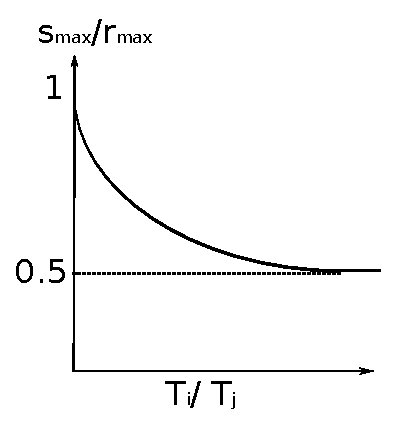
\includegraphics[scale=0.5]{figures/figure14}
\par\end{centering}
\caption{\label{fig14}Effect of $\left\lceil\frac{t(T_{i})}{t(T_{j})}\right\rceil$ on
$\frac{s_{max}}{r_{max}}$}
\end{figure}


\subsection{RCM versus Lock-Free}

\begin{clm}
For RCM's schedulability to be better or equal to that of~\cite{key-5}'s retry-loop lock-free approach, the size of $s_{max}$ must not exceed one half of that of $r_{max}$ for all cases.
However, the size of $s_{max}$ can be larger than that of $r_{max}$, depending on the number of accesses to a task $T_i$'s shared objects from other tasks.
\end{clm}
\begin{proof}\normalfont
Equation (\ref{eq20}) is upper bounded by:
 \begin{equation}
\sum_{\left(T_{j}\in\gamma_{i}\right)\wedge\left(p\left(T_{j}\right)> p\left(T_{i}\right)\right)}\left(\left\lceil\frac{t\left(T_{i}\right)-c_{j}}{t\left(T_{j}\right)}\right\rceil+1\right).2.\beta_{i,j}.s_{max}
\label{eq34}\end{equation}

Consider the same assumptions as in Section~\ref{sub:G-EDF-scheduler-with}.
Let \[\alpha_{rma}=\sum_{\left(T_{j}\in\gamma_{i}\right)\wedge\left(p\left(T_{j}\right)> p\left(T_{i}\right)\right)}\left(\left\lceil\frac{t\left(T_{i}\right)-c_{j}}{t\left(T_{j}\right)}\right\rceil+1\right).2.\beta_{i,j}\]Now, the ratio $s_{max}/r_{max}$ is upper bounded by:
\begin{equation}
\frac{s_{max}}{r_{max}}\le\frac{\sum_{T_{i}}\alpha_{free}/t\left(T_{i}\right)}{\sum_{T_{i}}\alpha_{rma}/t\left(T_{i}\right)}
\label{eq35}\end{equation}

The main difference between RCM and lock-free is that RCM is affected only by the higher priority tasks, while lock-free is affected by all tasks (just as in ECM). 
Besides, the RCM
is still affected by $2.\beta_{i,j}$ (just as in ECM).
The subtraction of $c_{j}$ in the numerator in (\ref{eq34}) may not
have a significant effect on the ratio of (\ref{eq35}), as the loop retry 
cost can also be modified to account for the effect of the first interfering
instance of task $T_{j}$. 
%%BR: In this paragraph, why don't you say "RCM" instead of "RMA CM"???


%%BR: Again, in the rest of this section, you can say "RCM" instead of "RMA CM"???
Therefore, 
$\alpha_{free} = \sum_{T_{j}\in\gamma_{i}}\left(\left\lceil\frac{t\left(T_{i}\right)-c_j}{t\left(T_{j}\right)}\right\rceil + 1 \right)\beta_{i,j}$.

Let tasks in the denominator of (\ref{eq35}) be given indexes $k$ instead of $i$, and $l$ instead of $j$. Let tasks in both the numerator and denominator of (\ref{eq35}) be arranged in the non-increasing priority order, so that $i=k$ and $j=l$. Let $\alpha_{free}$, in (\ref{eq35}), be divided into two parts: $\bar{\alpha}_{free}$ that contains only tasks with priority higher than $T_i$, and $\hat{\alpha}_{free}$ that contains only tasks with priority lower than $T_i$. Now, (\ref{eq35}) becomes:
\begin{eqnarray}
\frac{s_{max}}{r_{max}} & \le & \frac{\sum_{T_{i}}(\bar{\alpha}_{free}+\hat{\alpha}_{free})/t(T_{i})}{\sum_{T_{k}}\alpha_{rma}/t(T_{k})}\nonumber \\
 & = & \frac{1}{2}+\frac{\sum_{T_{i}}\hat{\alpha}_{free}/t(T_{i})}{\sum_{T_{k}}\alpha_{rma}/t(T_{k})}\label{eq36}\end{eqnarray}

For convenience, we introduce the following notations:
\begin{eqnarray}
\zeta_{1}& = & \sum_{T_{i}}\frac{\sum_{\left(T_{j}\in\gamma_{i}\right)\wedge\left(p\left(T_{j}\right)<p\left(T_{i}\right)\right)}\left(\left\lceil\frac{t\left(T_{i}\right)-c_{j}}{t\left(T_{j}\right)}\right\rceil+1\right)\beta_{i,j}}{t\left(T_{i}\right)}\nonumber\\
& = & \sum_{T_i} \hat{\alpha}_{free}/t(T_i)
\nonumber\\
\zeta_{2} 
& = & \sum_{T_{k}}\frac{\sum_{\left(T_{l}\in\gamma_{k}\right)\wedge\left(p\left(T_{l}\right)>p\left(T_{k}\right)\right)}\left(\left\lceil\frac{t\left(T_{k}\right)-c_{l}}{t\left(T_{l}\right)}\right\rceil+1\right)\beta_{k,l}}{t\left(T_{k}\right)}\nonumber\\
& = & \frac{1}{2}\sum_{T_k} \alpha_{rma}/t(T_k)\nonumber
\end{eqnarray}
$T_{j}$ is of lower priority than $T_{i}$, which means $D(T_{j})>D(T_{i})$. Under G-RMA, this means, $t(T_{j})>t(T_{i})$.
Thus, $\left\lceil\frac{t(T_{i})-c_{j}}{t(T_{j})}\right\rceil=1$ for
all $T_{j}$ and \[\zeta_{1}=\sum_{T_{i}}(\sum_{(T_{j}\in\gamma_{i})\wedge(p(T_{j})<p(T_{i}))}(2.\beta_{i,j}))/t(T_{i})\]
Since $\zeta_{1}$ contains all $T_{j}$ of lower priority than
$T_{i}$ and $\zeta_{2}$ contains all $T_{l}$ of higher priority than $T_{k}$, 
and tasks are arranged in the non-increasing priority order, then for each $T_{i,j}$, there exists $T_{k,l}$ such
that $i=l$ and $j=k$. Figure~\ref{fig:matrix-example} illustrates this, where 0 means that the pair $i,j$ 
%%BR: Whenever you say "...pair i,j,... say "...pair $(i,j)$...." The brackets help with clarity. Do this fix throughout. 
does not exist in $\zeta_{1}$,
and the pair $k,l$ does not exist in $\zeta_{2}$' (i.e., 
there is no task $T_l$ that is going to interfere with $T_k$ in $\zeta_2$), 
and 1 means the opposite. 

\begin{figure}[htbp]
\begin{tabular}{ccc}
$\begin{array}{cccccc}
 & j & 1 & 2 & \cdots & n\\
i\\
1 &  & 0 & 1 & \cdots & 1\\
2 &  & 0 & 0 & \ddots & \vdots\\
\vdots &  & \vdots & \vdots & \ddots & 1\\
n &  & 0 & 0 & \cdots & 0\end{array}$ &  & $\begin{array}{cccccc}
 & l & 1 & 2 & \cdots & n\\
k\\
1 &  & 0 & 0 & \cdots & 0\\
2 &  & 1 & 0 &  & \vdots\\
\vdots &  & \vdots & \ddots & \ddots & 0\\
n &  & 1 & \cdots & 1 & 0\end{array}$\tabularnewline
\end{tabular}
\caption{\label{fig:matrix-example} Task association for lower priority tasks than $T_i$ and higher priority tasks than $T_k$}
\end{figure}

Thus, it can be seen that both the matrices are transposes of
each other. Consequently, for each $\beta_{i,j}$, there exists $\beta_{k,l}$
such that $i=l$ and $j=k$. But the number of times $T_{j}$ accesses
a shared object with $T_{i}$ may not be the same as the number of times
$T_{i}$ accesses that same object. Thus, $\beta_{i,j}$ does not have
to be the same as $\beta_{k,l}$, even if $i,j$ and $k,l$ are transposes 
of each other. Therefore, we can analyze the behavior of $s_{max}/r_{max}$ based on the three parameters $\beta_{i,j}$, $\beta_{k,l}$, and $\left\lceil\frac{t(T_{k})-c_{l}}{t(T_{l})}\right\rceil$.
If $\beta_{i,j}$ is increased so that $\beta_{i,j}\rightarrow\infty$,
$\therefore\,(\ref{eq36})\rightarrow\infty$.
This is because, $\beta_{i,j}$ represents the number of times a lower priority task $T_{j}$ accesses 
shared objects with the higher priority task $T_{i}$. 
While this number has a greater effect in lock-free, it does not have any effect under RCM, because lower priority tasks do not affect higher priority
ones, so $s_{max}$ is allowed to be much greater than $r_{max}$.

Although the minimum value for $\beta_{i,j}$ is 1, mathematically, if $\beta_{i,j}\rightarrow0$, then $(\ref{eq36})\rightarrow1/2$.
Here, changing $\beta_{i,j}$ does not affect the retry cost of RCM, but it does affect the retry cost of lock-free, because the contention between tasks is reduced. Thus, $s_{max}$ is reduced in this case to
a little more than half of $r_{max}$ (``a little more''
because the minimum value of $\beta_{i,j}$ is actually 1, not 0).


The change of $s_{max}/r_{max}$ with respect to $\beta_{i,j}$ is shown in Figure~\ref{fig15-a}.
If $\beta_{k,l}\rightarrow\infty$, then (\ref{eq36})$\rightarrow1/2$.
This is because, $\beta_{k,l}$ represents the number of times
a higher priority task $T_{l}$ accesses shared objects with a lower
priority task $T_{k}$. Under RCM, this will increase the retry 
cost, thus reducing $s_{max}/r_{max}$. But if $\beta_{k,l}\rightarrow0$, then (\ref{eq36})$\rightarrow\infty$. This is due to the lower contention from a higher priority task $T_{l}$ to a lower priority task $T_{k}$, which reduces the retry cost under RCM and allows $s_{max}$ to be very large compared with $r_{max}$. Of course, the actual minimum value for $\beta_{k,l}$ is 1, and is illustrated in Figure~\ref{fig15-b}.

The third parameter that affects $s_{max}/r_{max}$ is $t(T_{k})/t(T_{l})$.
If $t(T_{l})\ll t(T_{k})$, then $\left\lceil\frac{t(T_{k})-c_{l}}{t(T_{l})}\right\rceil\rightarrow\infty$,
and $(\ref{eq36})\rightarrow1/2$. This is due to a high number
of interferences from a higher priority task $T_{l}$ to a lower priority
one $T_{k}$, which increases the retry cost under RMA CM, and consequently reduces $s_{max}/r_{max}$. 

If $t(T_{l})=t(T_{k})$ (which is
the maximum value for $t(T_{l})$ as $D(T_{l})\le D(T_{k})$, because
$T_{l}$ has a higher priority than $T_{k}$), then $\left\lceil\frac{t(T_{k})-c_{l}}{t(T_{l})}\right\rceil\rightarrow1$
and $\zeta_2=\sum_{T_{k}}\frac{\sum_{\left(T_{l}\in\gamma_{k}\right)\wedge\left(p\left(T_{l}\right)>p\left(T_{k}\right)\right)}2\beta_{k,l}}{t\left(T_{k}\right)}$. 
This means that the system will be controlled by only two parameters, $\beta_{i,j}$, and $\beta_{k,l}$, as in the previous two cases, shown in Figures~\ref{fig15-a} and~\ref{fig15-b}. Claim follows.
\end{proof}

\begin{figure}
\begin{centering}
\subfigure[\label{fig15-a}]{\begin{centering}
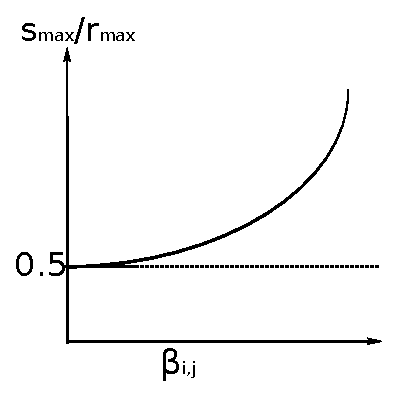
\includegraphics[scale=0.5]{figures/figure15-a}
\par\end{centering}
}\subfigure[\label{fig15-b}]{\begin{centering}
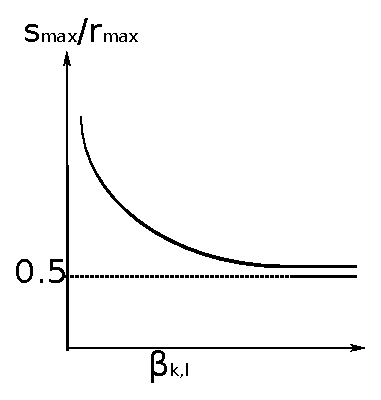
\includegraphics[scale=0.5]{figures/figure15-b}
\par\end{centering}
}
\par\end{centering}
\centering{}\caption{\label{fig15}Change of $s_{max}/r_{max}$: a) $\frac{s_{max}}{r_{max}}$
versus $\beta_{i,j}$ and b) $\frac{s_{max}}{r_{max}}$ versus $\beta_{k,l}$}
%%BR: I updated the caption, correct?
\end{figure}

\subsection{FMLP \& OMLP versus ECM and RCM
}

\begin{clm}
For ECM's schedulability to be better or equal to that of FMLP or OMLP, 
$s_{max}/|s\_\theta|_{max}$ (in case of FMLP), where $|s\_\theta|_{max}$ be the maximum short request by any task, and $s_{max}/L_{max}$ (in case of OMLP) must  not exceed $O(\frac{m}{n})$, where $L_{max}=max_{\forall i,\forall k}L_{i,k}$. For RCM's schedulability  
to be better or equal  
to that of OMLP, $s_{max}/L_{max}$ must not exceed $O(\frac{m}{n})$.
\end{clm}
\begin{proof}\normalfont
As FMLP is used with G-EDF (GSN-EDF), we compare only ECM 
against it. 
%%BR: "...we compare only ECM against it."??? 
First, we derive upper bounds for the blocking parameters of FMLP. When requests are non-nested, each resource (short or long) will be contained in its own group. Let $N_{i,s}$ be the number of times a task $T_{i}$ requests a short
resource, $|s\_\theta|_{i,max}$ be the maximum request for a
short resource by $T_{i}$, $\alpha_{bw}=N_{i,s}.(m-1)$. Now, FMLP's three  blocking terms, described in Section~\ref{global-fmlp}, are upper bounded as follows:
\begin{eqnarray*}
BW(T_{i}) & \le & \sum_{s\_\theta\in\theta_{i}}(m-1).|s\_\theta|_{i,max}\\
 & = & N_{i,s}.(m-1).|s\_\theta|_{i,max}\\
 & \le & N_{i,s}.(m-1).|s\_\theta|_{max}\\
& = & \alpha_{bw}.|s\_\theta|_{max}
 \end{eqnarray*}
\begin{eqnarray*}
NPB\left(T_{i}\right) & \le & \left(1+N_{i,l}\right).max\left(BW_{k\ne i}\left(T_{k}\right)+|s\_\theta|_{k,max}\right)\\
 & \le & \left(1+N_{i,l}\right).max\left(BW_{k\ne i}\left(T_{k}\right)+|s\_\theta|_{max}\right)\\
 & = & \left(1+N_{i,l}\right).|s\_\theta|_{max}.max_{k\ne i}\left(N_{k,s}.\left(m-1\right)+1\right)\\
 & = & \alpha_{npb}.|s\_\theta|_{max}
 \end{eqnarray*}
 where $\alpha_{npb}=\left(1+N_{i,l}\right).max_{k\ne i}\left(N_{k,s}.\left(m-1\right)+1\right)$.
\begin{eqnarray*}
DB\left(T_{i}\right) & \le & N_{i,l}.\left(n-1\right).|l\_\theta|_{i,max}\\
 & \le & N_{i,l}.\left(n-1\right).|l\_\theta|_{max}\\
 \end{eqnarray*}
If $|l\_\theta|_{max}\le c1.|s\_\theta|_{max}$, where $c1$ is the
minimum constant that satisfies this relation, then
\begin{eqnarray*}
DB\left(T_{i}\right)& \le & N_{i,l}.\left(n-1\right).c1.|s\_\theta|_{max}\\
& = & \alpha_{db}.|s\_\theta|_{max}
\end{eqnarray*}
where $\alpha_{db}=N_{i,l}.\left(n-1\right).c1$. 

The total blocking time of each task is added to the task execution time, and
as before, we compare the total utilization of the G-EDF system (with both contention managers) against that under FMLP. 

Now, for ECM's schedulability to be better than FMLP,
\begin{equation}
 \frac{s_{max}}{|s\_\theta|_{max}}\le
 \frac{\sum_{T_{i}}\left(\alpha_{bw}+\alpha_{npb}+\alpha_{db}\right) \Big/t(T_{i})}{\sum_{T_{i}}\alpha_{edf} \Big/t(T_{i})}
 \label{eq38} \end{equation}

From (\ref{eq38}), it can be seen that $T_{i}$'s blocking time,
under FMLP, depends on $m,\, n$ and the number of times it requests resources
(in contrast to ECM, 
%%BR: "...contrast to ECM,..."???  
under which, $T_i$'s retry cost depends on the number of times a conflicting task $T_{j}$ requests resources). Thus, if $N_{i,s},\, N_{i,l}$, 
and $N_{k,s}$ can all be upper bounded by some constant $C_{2}$,
which is the maximum number of times any task $T_{i}$ can request a short
or long resource, then the numerator in (\ref{eq38}) 
is $O(n(n+m))$, while the denominator is $O(n^{2})$. Therefore:
\begin{equation}
\frac{s_{max}}{|s\_\theta|_{max}}=O\left(\frac{m}{n} \right)
\label{eq45}
\end{equation}
This means that, for $n<m$, the contention between tasks under both STM and
FMLP is low (even for short resources under FMLP), but FMLP is more affected
by $NTB$. When $n>m$, contention increases, but FMLP arranges
requests in a FIFO queue, so it is less affected than ECM, 
%%BR: "..than ECM,...???
which
suffers from conflicting tasks and instances
of each conflicting one. FMLP is not affected by the number of instances
of each conflicting task.

%%%%
Since OMLP's blocking time is bounded by (\ref{eq29}) \[ \therefore 
%\;
bi\le2.\left(m-1\right).L_{max}\sum_{k=1}^{q}N_{i,k}\]
%%BR: THis sentence is awkward. Why don't you say "Let  \[L_{max}=..... Since OMLP's blocking time is ..., \therefore.."


For ECM's schedulability to be better than global OMLP:
\begin{equation}
\frac{s_{max}}{L_{max}}\le\frac{\sum_{T_{i}}\left(2.\left(m-1\right)\sum_{k=1}^{q}N_{i,k}\right) \Big/t\left(T_{i}\right)}{\sum_{T_{i}}\alpha_{edf} \Big/t\left(T_{i}\right)}\label{eq40}\end{equation}

For RCM, the ratio is:
\begin{equation}
\frac{s_{max}}{L_{max}}\le\frac{\sum_{T_{i}}\left(2.\left(m-1\right)\sum_{k=1}^{q}N_{i,k}\right) \Big/t\left(T_{i}\right)}{\sum_{T_{i}}\alpha_{rma} \big/t\left(T_{i}\right)}\label{eq41}\end{equation}


If $\sum_{k=1}^{q}N_{i,k}$ is upper bounded by $C_{3}$, which is
a constant representing the maximum total number of requests for resources
by any task $T_{i}$, then:
\begin{equation}
\frac{s_{max}}{L_{max}}=O\left(\frac{nm}{n^{2}}\right)=O\left(\frac{m}{n}\right)
\label{eq46}
\end{equation}
for each of (\ref{eq40}) and (\ref{eq41}). Claim follows.
\end{proof}

\section{\label{FIFO}Response time of G-EDF and G-RMA system with FIFO CM}

In FIFO CM, transactions are executed in the order they arrive. This
way, the effect of an atomic section of $T_{j}$ to one in $T_{i}$
is shown in Figure \ref{fig12-a} for early validation and Figure
\ref{fig12-b} for lazy validation. In both cases, $s_{i}^{l}(\theta)$
must retry for at most $len(s_{j}^{p}(\theta))$, which is less than
that of EDF CM and RMA CM, but a higher priority task can be delayed
by a lower one if the latter's atomic section arrives earlier than
the former. Besides, if a low priority task, $T_i$, is executing its atomic section, and a higher priority one, $T_j$, is released and allocated to the processor of $T_i$, the order of the atomic section of $T_i$ in the FIFO is delayed after any conflicting atomic section arrives in the preemption interval of $T_i$, otherwise, tasks other than $T_i$ can be delayed until $T_i$ is allocated a processor again and finishes its atomic section, besides this helps avoiding deadlocks, as $T_j$ itself may need to access the same object accessed by the atomic section of $T_i$ but it cannot commit because every time it tries to do that, CM will enforce it to abort as it arrives later than the atomic section of the preempted task.

%
\begin{figure}
\centering{}\subfigure[\label{fig12-a}]{\centering{}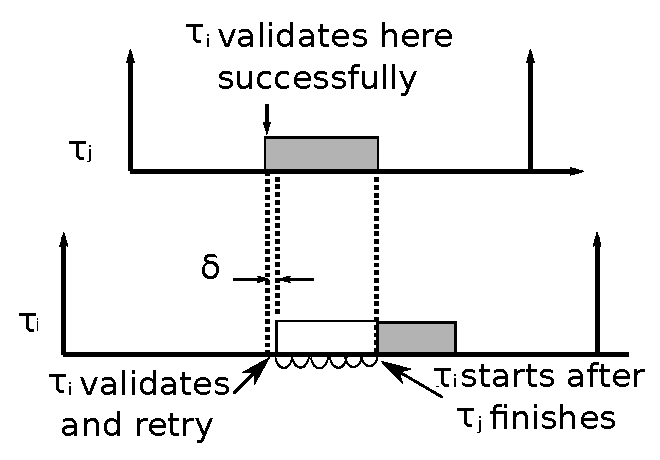
\includegraphics[scale=0.4]{figures/figure12-a}}\subfigure[\label{fig12-b}]{\centering{}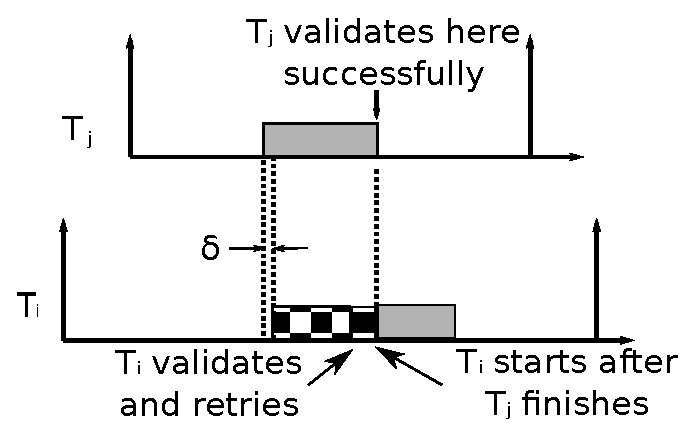
\includegraphics[scale=0.4]{figures/figure12-b}}\caption{\label{fig12}(a)Early validation (b)Lazy validation}

\end{figure}


Retrial of atomic sections here does not depend on the scheduler,
rather it only depends on the arrival pattern, so retrial
cost ($RC$) will be the same for both G-EDF and G-RMA
systems, and the maximum pattern of interference will also be the
same as shown in Figure \ref{fig11} (in case of G-EDF, the last instance of the interfering task with longer absolute deadline than the studied one, can have atomic sections arriving earlier than that of $T_i$ and still conflict with them), but this pattern differs when calculating the contribution of other tasks during the non-atomic part of $T_{i}$.

$RC$ can be calculated by (\ref{eq23})\begin{eqnarray}
\hat{RC}(L(T_{i})) & = & \sum_{\theta\in\theta_{i}}((\sum_{T_{j}\in\gamma(\theta)}((\lceil\frac{L-c_{j}}{t(T_{j})}\rceil+1).\nonumber \\
 &  & \sum_{\forall s_{j}^{l}(\theta)}len(s_{j}^{l}(\theta)))))\label{eq23}\end{eqnarray}
where the lengths of all atomic sections in all tasks that share object
$\theta$ with $T_{i}$ are summed together, and $L$ can extend to
cover $t(T_{i})$. It should be noted that one instance can have multiple
atomic sections that access the same object, then how can an atomic
section of $T_{i}$ be interfered by all of them while it should be
interfered by only one of them according to its arrival time, as the
others will come after that of $T_{i}$? This can happen if $T_{i}$
was trying to execute its atomic section, then it is replaced by a
higher priority job, then $T_{i}$ gets back to the processor. In
the time of preemption, another atomic section of the same conflicting
task can come and execute. This situation is shown in Figure \ref{fig13}
where $s_{i}^{l}$ retries while $s_{j}^{p}$ is executing, then $T_{k}$
is released, preempting $T_{i}$ to get its processor and before it
finished, $s_{j}^{p+1}$ executes, so when $s_{i}^{l}$ returns after
$T_{k}$ finishes, it will be after $s_{j}^{p+1}$ and it will have
to retry until it finishes. For this, (\ref{eq23}) sums the lengths
of all atomic sections in each instance that access the same object
as the studied task.

%
\begin{figure}
\centering{}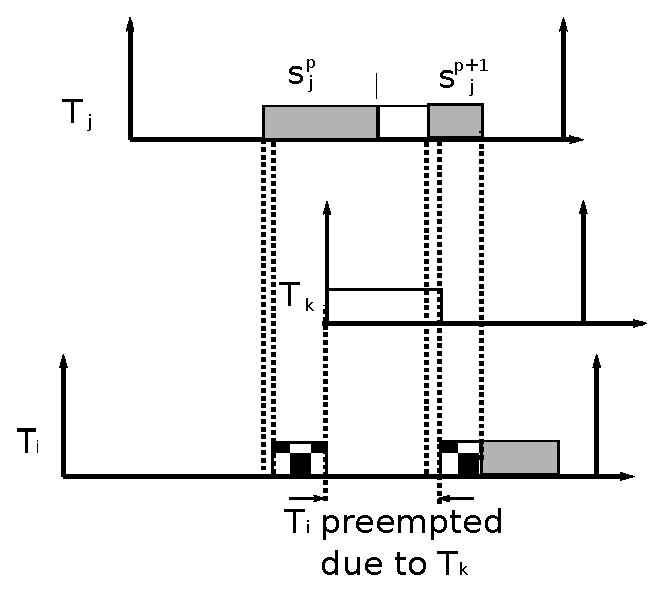
\includegraphics[scale=0.5]{figures/figure13}\caption{\label{fig13}Retrial of $s_{i}^{l}$ by multiple atomic sections of $s_{j}^{p}$}
\end{figure}



The rest of analysis for both schedulers is done as before, only $RC(L(T_{i}))$
is changed.

\textbf{\textit{\underbar{In case of G-RMA}}}

For G-RMA, the case shown in Figure \ref{fig13} can happen only if $T_{i}$ is the lowest
priority among all running tasks, which reduces number of conflicting
tasks to only those of higher or equal priority to that of $T_{i}$.
Meanwhile, if there are $m$ processors, this means that before $T_{i}$
gets preempted, it will retry for the duration of at most the maximum
$m-1$ atomic sections sharing the same object with $T_{i}$ whether they belong to higher priority tasks or not.

After $T_{i}$ gets preempted, no lower priority task can allocate
a processor while $T_{i}$ is waiting, but as $T_{i}$ can get preempted
again and again by higher priority tasks, it can be delayed for each release of a higher priority
job, $T_{i}$ by the maximum $m-1$ higher or equal priority tasks (the first term of the "min" part in (\ref{eq24})), or, it can be delayed by the sum of all atomic sections in higher priority tasks that access the same object as $T_{i}$ (the second term of the ``min'' part in (\ref{eq24})).

So, $RC$ in the case of G-RMA can be calculated as in
(\ref{eq24})

\begin{eqnarray}
RC^{*}(L(T_{i}))= & \sum_{\theta\in\theta_{i}}(\sum_{k=1}^{min(n-1,m-1)}(\omega(k,\theta))+\nonumber \\
(\sum_{T_{j}^*}min^* & \begin{cases}
\lceil\frac{L}{t(T_{j})}\rceil.\sum_{k=1}^{m-1}\omega_{high}(k,\theta)))\\
(\lceil\frac{L-c_{j}}{t(T_{j})}\rceil+1).\sum_{\forall s_{j}^{l}(\theta)}len(s_{j}^{l}(\theta))))\end{cases}\label{eq24}\end{eqnarray}



where:-
\begin{itemize}
\item $\omega(k,\theta)$ is the set of $s_{p_{max}}(\theta), p \ne i $ arranged
in non-increasing order. 
\item $\omega_{high}(k,\theta)$ is the set of $s_{p_{max}}(\theta), p \ne i $ arranged
in non-increasing order, where $p(T_{p})\ge p(T_{i})$.
\item $min^* = 0$ if $n\le m$.
\item $T_j^* = \{T_j|(T_{j}\in\gamma(\theta))\wedge(p(T_{j})\ge p(T_{i}))\}$.
\end{itemize}
The second term is zero in case number of tasks is less than or equal
to number of processors, because $T_{i}$ will not have to be preempted
because of enough number of processors for tasks, and the final value for retrial cost will be the minimum of (\ref{eq23}) and (\ref{eq24}).
\begin{equation}
RC(L(T_i))=min(\hat{RC}(L(T_i)),RC^{*}(L(T_i)))\label{eq26}
\end{equation}
 The rest of the
analysis for workload of other tasks is the same as before.

\textbf{\textit{\underbar{In case of G-EDF}}}

G-EDF is similar to G-RMA in that $T_{i}$- before it is preempted-
it can be delayed by the maximum $min(m-1,n-1)$ tasks, but after it is preempted, no task of longer, or equal, relative deadline
than $T_{i}$ will start before it because it will have a longer absolute
deadline. So, $RC$ in the case of G-EDF will be calculated
as shown in (\ref{eq25}) where $L$ can be extended to $t(T_{i})$, and the final $RC$ will be calculated as in (\ref{eq26}).

\begin{eqnarray}
RC^{*}(L(T_{i}))= & \sum_{\theta\in\theta_{i}}(\sum_{k=1}^{min(n-1,m-1)}(\omega(k,\theta))+\nonumber \\
(\sum_{T_{j}^{*}}min^* & \begin{cases}
\lfloor\frac{L}{t(T_{j})}\rfloor.\sum_{k=1}^{m-1}\omega_{high}(k,\theta))\\
(min\begin{cases}
\lceil\frac{L-c_{j}}{T_{j}}\rceil+1\\
\lfloor\frac{T_{i}}{T_{j}}\rfloor\end{cases}).\sum_{\forall s_{j}^{l}(\theta)}len(s_{j}^{l}(\theta))))\end{cases}\label{eq25}\end{eqnarray}

where:-
\begin{itemize}
\item $min^* =0$ if $n\le m$.
\item $T_{j}^{*}=\{T_{j}|(T_{j}\in\gamma(\theta))\wedge(D(T_{j})\le D(T_{i})\}$
\item The ``$min$'' term in ``$min^{*}$'' accommodates for the right number of interference of higher priority tasks during the period $L$ (the top term), or the whole period of $T_i$ (the bottom term) as explained before in the analysis of G-EDF with EDF CM.
\end{itemize}

Workload of other tasks is the same as before.


\section{Length-based CM}

LCM resolves conflicts based on the priority of conflicting jobs, besides the length of the interfering atomic section, and the length of the interfered atomic section. This is in contrast to ECM and RCM~\cite{stmconcurrencycontrol:emsoft11}, where conflicts are resolved using the priority of the conflicting jobs. This strategy allows lower priority jobs, under LCM, to retry for lesser time than that under ECM and RCM, but higher priority jobs, sometimes, wait for lower priority ones with bounded priority-inversion.

\subsection{\label{sec 9.1} Design and Rationale}

%Begin algorithm here
\begin{algorithm}
\footnotesize{
\LinesNumbered
\KwData{$s_i^k(\theta)\rightarrow$ interfered atomic section.\\$s_j^l(\theta)\rightarrow$ interfering atomic section.\\$\psi\rightarrow$ predefined threshold $\in [0,1]$.\\$\delta_i^k(\theta)\rightarrow$ remaining execution length of $s_i^k(\theta)$}
\KwResult{which atomic section of $s_i^k(\theta)$ or $s_j^l(\theta)$ aborts}
\eIf{$p_i^k > p_j^l$}
	{$s_j^l(\theta)$ aborts\label{step_sicommits}\;}
	{$c_{ij}^{kl}=len(s_j^l(\theta))/len(s_i^k(\theta))$\label{step_cijkl}\;
	$\alpha_{ij}^{kl}=ln(\psi)/(ln(\psi)-c_{ij}^{kl})$\label{step_alphaijkl}\;
	$\alpha=\left(len(s_i^k(\theta))-\delta_i^k(\theta)\right)/len(s_i^k(\theta))$\;
	\eIf{$\alpha \le \alpha_{ij}^{kl}$}
	{$s_i^k(\theta)$ aborts\label{step_siaborts}\;}
	{$s_j^l(\theta)$ aborts\label{step_sjaborts}\;}
	}
	}
\caption{LCM}
\label{alg_lcm}
\end{algorithm}
%End algorithm here

For both ECM and RCM, $s_{i}^{k}(\theta)$ can be totally repeated if $s_{j}^{l}(\theta)$ --- which belongs to a higher priority job $\tau_{j}^b$ than $\tau_{i}^a$ --- conflicts with $s_{i}^{k}(\theta)$
at the end of its execution, while $s_{i}^{k}(\theta)$ is just about
to commit. Thus, LCM, shown in Algorithm~\ref{alg_lcm}, uses the remaining length of $s_{i}^{k}(\theta)$ when it is interfered,
as well as $len(s_{j}^{l}(\theta))$, to decide which transaction must be aborted. If $p_i^k$ was greater than $p_j^l$, then $s_i^k(\theta)$ would be the one that commits, because it belongs to a higher priority job, and it started before $s_j^l(\theta)$ (step~\ref{step_sicommits}). Otherwise, $c_{ij}^{kl}$ is calculated (step~\ref{step_cijkl}) to determine whether it is worth aborting $s_i^k(\theta)$ in favor of $s_j^l(\theta)$, because $len(s_j^l(\theta))$ is relatively small compared to the remaining execution length of $s_i^k(\theta)$  (explained further).

We assume that:
\begin{equation}
c_{ij}^{kl}=len(s_{j}^{l}(\theta))/len(s_{i}^{k}(\theta))
\label{cm_eq}\end{equation}
where $c_{ij}^{kl}\in]0,\infty[$, to cover all possible lengths of $s_{j}^{l}(\theta)$.
Our idea is to reduce the opportunity for the abort of $s_{i}^{k}(\theta)$ if it is close to committing when interfered and $len(s_{j}^{l}(\theta))$ is large. This abort opportunity is increasingly reduced as $s_{i}^{k}(\theta)$ gets closer to the end of its execution, or $len(s_{j}^{l}(\theta))$ gets larger. 

On the other hand, as $s_{i}^{k}(\theta)$ is interfered early,
or $len(s_{j}^{l}(\theta))$ is small compared to $s_{i}^{k}(\theta)$'s remaining length, the abort opportunity 
is increased even if $s_i^k (\theta)$ is close to the end of its execution. To decide whether $s_{i}^{k}(\theta)$ must be aborted or not, we use a threshold value $\psi\in[0,1]$ that determines $\alpha_{ij}^{kl}$ (step~\ref{step_alphaijkl}), where $\alpha_{ij}^{kl}$ is the maximum percentage of $len(s_i^k(\theta))$ below which $s_j^l(\theta)$ is allowed to abort $s_i^k(\theta)$. Thus, if the already executed part of $s_i^k(\theta)$ --- when $s_j^l(\theta)$ interferes with $s_i^k(\theta)$ --- does not exceed $\alpha_{ij}^{kl}len(s_i^k(\theta))$, then $s_i^k(\theta)$ is aborted (step~\ref{step_siaborts}). Otherwise, $s_j^l(\theta)$ is aborted (step~\ref{step_sjaborts}).

%
\begin{figure}[htbp]
\centering
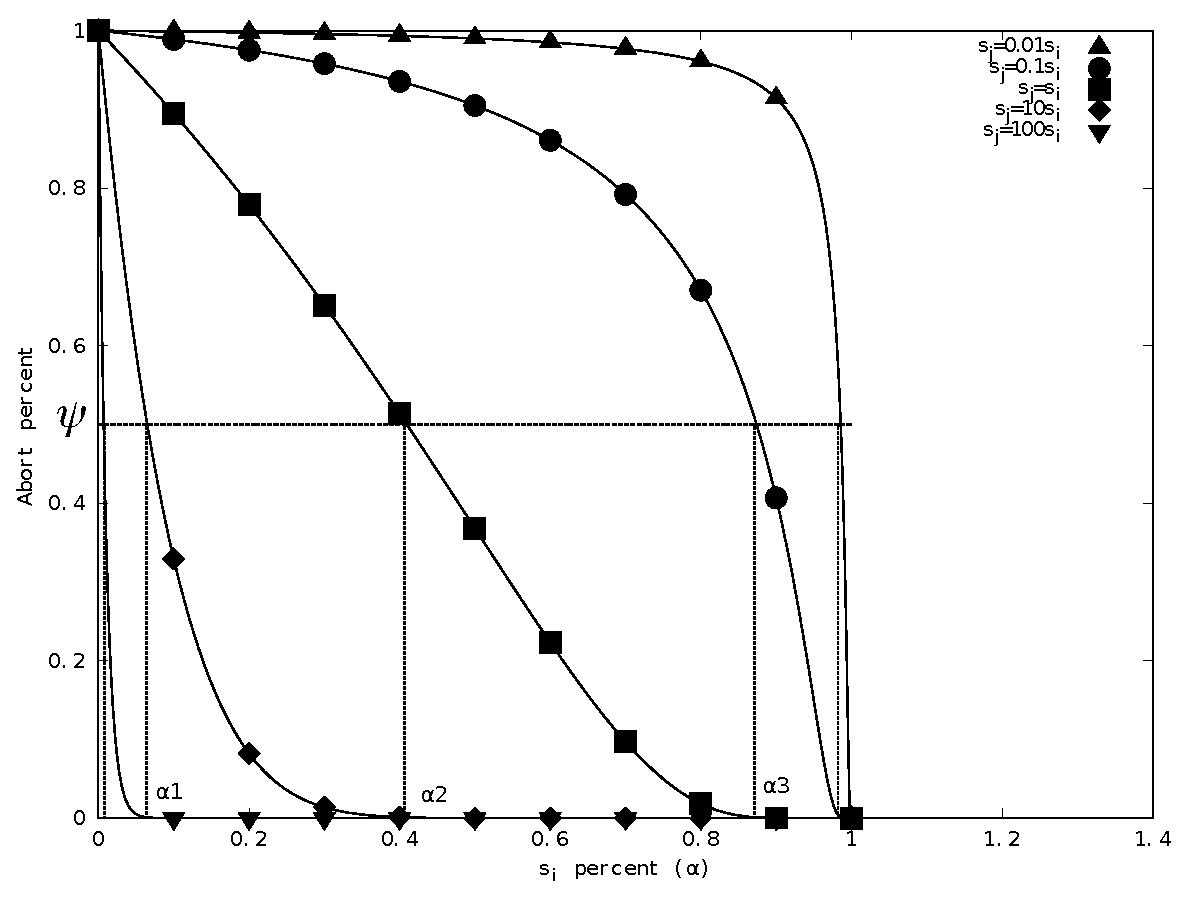
\includegraphics[scale=0.4]{figures/figure16}
\caption{\label{fig16}Interference of $s_{i}^{k}(\theta)$ by various lengths of 
$s_{j}^{l}(\theta)$}
\end{figure}

The behavior of LCM is illustrated in Figure~\ref{fig16}. In this figure, the horizontal axis corresponds to different values of $\alpha$ ranging from $0$ to $1$, and the vertical axis corresponds to different values of abort opportunities, $f(c_{ij}^{kl},\alpha)$, ranging from $0$ to $1$ and calculated by~(\ref{eq49}):
\begin{equation}
f(c_{ij}^{kl},\alpha)=e^{\frac{-c_{ij}^{kl}\alpha}{1-\alpha}}
\label{eq49}\end{equation}
where $c_{ij}^{kl}$ is calculated by~(\ref{cm_eq}).

Figure~\ref{fig16} shows one atomic section $s_i^k(\theta)$ (whose $\alpha$ changes along the horizontal axis) interfered by five different lengths of $s_j^l(\theta)$.
For a predefined value of $f(c_{ij}^{kl},\alpha)$ (denoted as $\psi$ in Algorithm~\ref{alg_lcm}), there corresponds a specific value of $\alpha$ (which is $\alpha_{ij}^{kl}$ in Algorithm~\ref{alg_lcm}) for each curve. For example, when $len(s_j^l(\theta))=0.1 \times len(s_i^k(\theta))$, $s_j^l(\theta)$ aborts $s_i^k(\theta)$ if the latter has not executed more than $\alpha3$ percentage (shown in Figure~\ref{fig16}) of its execution length. As $len(s_{j}^{l}(\theta))$ decreases, the corresponding $\alpha_{ij}^{kl}$ increases (as shown in Figure~\ref{fig16}, $\alpha3>\alpha2>\alpha1$).

Equation (\ref{eq49}) achieves the desired requirement that the abort opportunity is reduced as $s_{i}^{k}(\theta)$ gets
closer to the end of its execution (as $\alpha\rightarrow1,\, f(c_{ij}^{kl},1)\rightarrow0$),
or as the length of the conflicting transaction increases (as $c_{ij}^{kl}\rightarrow\infty,\, f(\infty,\alpha)\rightarrow0$).
Meanwhile, this abort opportunity is increased as $s_{i}^{k}(\theta)$
is interfered closer to its release (as $\alpha\rightarrow0,\, f(c_{ij}^{kl},0)\rightarrow1$),
or as the length of the conflicting transaction decreases (as $c_{ij}^{kl}\rightarrow0,\, f(0,\alpha)\rightarrow1$).

LCM is not a centralized CM, which means that, upon a conflict, each transactions has to decide whether it must commit or abort. 

\begin{clm}
\label{LCM_higher_rc}
Let $s_{j}^{l}(\theta)$ interfere once with $s_{i}^{k}(\theta)$ at $\alpha_{ij}^{kl}$. Then, the maximum contribution of $s_{j}^{l}(\theta)$ to 
$s_{i}^{k}(\theta)$'s 
retry cost is:
\begin{equation}
W_i^k(s_j^l(\theta))\le \alpha_{ij}^{kl}len\Big(s_{i}^{k}(\theta)\Big)+len\Big(s_{j}^{l}(\theta)\Big)\label{eq47}\end{equation}
\end{clm}

\begin{proof}\normalfont
If $s_{j}^{l}(\theta)$ interferes with $s_{i}^{k}(\theta)$
at a $\Upsilon$ percentage, where $\Upsilon<\alpha_{ij}^{kl}$,
then the retry cost of $s_{i}^{k}(\theta)$ is $\Upsilon len(s_{i}^{k}(\theta))+len(s_{j}^{l}(\theta))$, which is lower than that calculated in (\ref{eq47}). Besides, 
if $s_{j}^{l}(\theta)$ interferes with $s_{i}^{k}(\theta)$ after
$\alpha_{ij}^{kl}$ percentage, then $s_{i}^{k}(\theta)$ will not
abort.
\end{proof}


\begin{clm}
\label{LCM_lower_rc}
An atomic section of a higher priority job, $\tau_{j}^b$, may have to abort and retry due to a lower priority job, $\tau_{i}^a$, if $s_{j}^{l}(\theta)$ interferes
with $s_{i}^{k}(\theta)$ after the $\alpha_{ij}^{kl}$ percentage. $\tau_{j}$'s retry time, due to $s_{i}^{k}(\theta)$ and $s_{j}^{l}(\theta)$,
is upper bounded by:
 \begin{equation}
W_j^l(s_i^k(\theta))\le \Big(1-\alpha_{ij}^{kl}\Big)len\Big(s_{i}^{k}(\theta)\Big)\label{eq48}\end{equation}
\end{clm}

\begin{proof}\normalfont
It is derived directly from Claim~\ref{LCM_higher_rc}, as $s_j^l(\theta)$ will have to retry for the remaining length of $s_i^k(\theta)$.
\end{proof}

%sh-start
\begin{clm}
\label{no priority inversion in lcm}
Under LCM, there is no priority inversion.
\end{clm}

\begin{proof}\normalfont
Assume three atomic sections, $s_i^k(\theta)$, $s_j^l(\theta)$, and $s_a^b(\theta)$, where $p_j > p_i$ and $s_j^l(\theta)$ interferes with $s_i^k(\theta)$ after $\alpha_{ij}^{kl}$. Then, $s_j^l(\theta)$ will have to abort and retry. At this time, if $s_a^b(\theta)$ interferes with the other two atomic sections, then LCM decides which transaction to commit by comparing the two transactions. So, we have the following cases:
\begin{itemize}
\item $p_a < p_i < p_j$. Now, $s_a^b(\theta)$ will not abort any one because it is still in its beginning and it is of the lowest priority. Thus, $\tau_j$ is not indirectly blocked by $\tau_a$.
\item $p_i<p_a<p_j$. Now, even if $s_a^b(\theta)$ interferes with $s_i^k(\theta)$ before $\alpha_{ia}^{kb}$,  and $s_a^b(\theta)$ is allowed to abort $s_i^k(\theta)$, after comparing $s_j^l(\theta)$ and $s_a^b(\theta)$, LCM will select $s_j^l(\theta)$ to commit and abort $s_a^b(\theta)$, because the latter is still at its beginning, and $\tau_j$ is of higher priority. If $s_a^b(\theta)$ is not allowed to abort $s_i^k(\theta)$, the situation is still the same, because $s_j^l(\theta)$ was already retrying until $s_i^k(\theta)$ finishes. So, the medium priority instance of $\tau_a$ does not increase the delay time of the higher priority instance of $\tau_j$.
%
\item $p_a>p_j>p_i$. Now, if $s_a^b(\theta)$ is chosen to commit, this will not cause a priority inversion for $\tau_j$ because $\tau_a$ is of higher priority.
\item if $\tau_a$ preempts $\tau_i$, then LCM will compare only between $s_j^l(\theta)$ and $s_a^b(\theta)$. If $p_a<p_j$, then $s_j^l(\theta)$ will commit because of its task's higher priority and $s_a^b(\theta)$ is still at its beginning. Otherwise, $s_j^l(\theta)$ will retry, but this will not be priority inversion, because $\tau_a$ is already of higher priority than $\tau_j$. If $\tau_a$ does not access any object but it preempts $\tau_i$, then LCM will choose $s_j^l(\theta)$ to commit, since only already running transactions are competing together.
\end{itemize}
%
From the previous cases, it appears that priority inversion can never happen under LCM. Claim follows.
\end{proof}

\begin{clm}
\label{priority_inversion}
A higher priority job, $\tau_j^v$, can be delayed by lower priority jobs for at most number of atomic sections in $\tau_j^v$.
\end{clm}

\begin{proof}\normalfont
By generalizing the cases mentioned in the proof of Claim~\ref{no priority inversion in lcm} to any number of conflicting jobs, it can be seen that when an atomic section, $s_j^l(\theta)$, of a higher priority job conflicts with a number of atomic sections belonging to lower priority jobs, $s_j^l(\theta)$ can be delayed only one of them, $s_i^k(\theta)$, for the remaining length of $s_i^k(\theta)$, then $s_j^l(\theta)$ can run. Thus, the worst case scenario happens when each atomic section in the higher priority job is delayed by one of the atomic sections belonging to lower priority jobs. Claim follows.
\end{proof}
%sh-end


\begin{clm}
\label{max_pri_inv}
The maximum delay suffered by $s_j^l(\theta)$ due to lower priority jobs is caused by the maximum length atomic section accessing object $\theta$, which belongs to a lower priority job than $\tau_j^b$ that owns $s_j^l(\theta)$.
\end{clm}

\begin{proof}\normalfont
Assume three atomic sections, $s_i^k(\theta)$, $s_j^l(\theta)$, and $s_h^z(\theta)$, where $p_j>p_i$, $p_j>p_h$, and $len(s_i^k(\theta))>len(s_h^z(\theta))$. Now, $\alpha_{ij}^{kl}>\alpha_{hj}^{zl}$ and $c_{ij}^{kl}<c_{hj}^{zl}$. By applying~(\ref{eq48}) to obtain the contribution of $s_i^k(\theta)$ and $s_h^z(\theta)$ to the priority inversion of $s_j^l(\theta)$ and dividing them, we get:
\begin{eqnarray*}
\frac{W_{j}^{l}(s_{i}^{k}(\theta))}{W_{j}^{l}(s_{h}^{z}(\theta))} & = & \frac{\left(1-\alpha_{ij}^{kl}\right)len(s_{i}^{k}(\theta))}{\left(1-\alpha_{hj}^{zl}\right)len(s_{h}^{z}(\theta))}
\end{eqnarray*}
By substitution for $\alpha$s from~(\ref{eq49}):
\begin{eqnarray*}
 & = & \frac{(1-\frac{ln\psi}{ln\psi-c_{ij}^{kl}})len(s_{i}^{k}(\theta))}{(1-\frac{ln\psi}{ln\psi-c_{hj}^{zl}})len(s_{h}^{z}(\theta))}
  =  \frac{(\frac{-c_{ij}^{kl}}{ln\psi-c_{ij}^{kl}})len(s_{i}^{k}(\theta))}{(\frac{-c_{hj}^{zl}}{ln\psi-c_{hj}^{zl}})len(s_{h}^{z}(\theta))}\end{eqnarray*}
$\because ln\psi \le 0$ and $c_{ij}^{kl},c_{hj}^{kl} > 0, \therefore$ by substitution from~(\ref{cm_eq})
\begin{eqnarray*}
 & = & \frac{len(s_{j}^{l}(\theta))/(ln\psi-c_{ij}^{kl})}{len(s_{j}^{l}(\theta))/(ln\psi-c_{hj}^{zl})}
  =  \frac{ln\psi-c_{hj}^{zl}}{ln\psi-c_{ij}^{kl}}>1\end{eqnarray*}
Thus, as the length of the interfered atomic section increases, the delay suffered by the interfering atomic section increases. Claim follows.
\end{proof}


\subsection{\label{response g-edf/lcm} Response Time of G-EDF/LCM}

%Toward establishing the response time under G-EDF/LCM, we introduce a set of claims.

\begin{clm}\label{GEDF/LCM response time}
$RC(T_i)$ for a task $\tau_i$ under G-EDF/LCM is upper bounded by:
\begin{eqnarray}
RC(T_i) & = & \Bigg(\sum_{\forall \tau_h \in \gamma_i}\sum_{\forall\theta \in \theta_i \wedge \theta_h}\Bigg(\left\lceil\frac{T_{i}}{T_{h}}\right\rceil\sum_{\forall s_{h}^{l}(\theta)}len\Big(s_{h}^{l}(\theta)\Big)\nonumber\\
& + & \alpha_{max}^{hl}len\Big(s_{max}^{h}(\theta)\Big)\Bigg)\Bigg)\nonumber\\
& + & \sum_{\forall s_{i}^{y}(\theta)}\Big(1-\alpha_{max}^{iy}\Big)len\Big(s_{max}^i(\theta)\Big)  
\label{eq78}\end{eqnarray} 
where $\alpha_{max}^{hl}$ is the $\alpha$ value that corresponds to $\psi$ due to the interference of $s_{max}^h(\theta)$ by $s_h^l(\theta)$. $\alpha_{max}^{iy}$ is the $\alpha$ value that corresponds to $\psi$ due to the interference of $s_{max}^i(\theta)$ by $s_i^y(\theta)$.
\end{clm}

\begin{proof}\normalfont
The maximum number of higher priority instances of $\tau_h$ that can interfere with $\tau_i^x$ is $\left\lceil\frac{T_i}{T_h}\right\rceil$, as shown in Figure~\ref{fig17}, where one instance of $\tau_h$ and $\tau_h^p$ coincides with the absolute deadline of $\tau_i^x$.

By using Claims~\ref{LCM_higher_rc},~\ref{LCM_lower_rc},~\ref{priority_inversion}, and~\ref{max_pri_inv}, and Claim 1 in~\cite{stmconcurrencycontrol:emsoft11} to determine the effect of atomic sections belonging to higher and lower priority instances of interfering tasks to $\tau_i^x$, Claim follows.
\end{proof}


Response time of $\tau_{i}$ is calculated by (11) in~\cite{stmconcurrencycontrol:emsoft11}.
\begin{figure}
\begin{centering}
\includegraphics[scale=0.6]{figures/figure18}
\par\end{centering}
\caption{\label{fig17}$\tau_h^p$ has a higher priority than $\tau_i^x$}
\end{figure}

\subsection{Schedulability of G-EDF/LCM and ECM}
\label{performance g-edf-lcm}
We now compare the schedulability of G-EDF/LCM with ECM~\cite{stmconcurrencycontrol:emsoft11} %(FMLP and OMLPprotocols~\cite{key-4,brandenburg2008comparison,key-3}), 
to understand when G-EDF/LCM will perform better. 
Toward this, we compare the total utilization of ECM with that of G-EDF/LCM. For each method, we inflate the $c_i$ of each task $\tau_i$ by adding the retry cost suffered by $\tau_i$. Thus, if method $A$ adds retry cost $RC_A(T_i)$ to $c_i$, and method $B$ adds retry cost $RC_B(T_i)$ to $c_i$, then the schedulability of $A$ and $B$ are compared as:
\begin{eqnarray}
\sum_{\forall \tau_{i}}\frac{c_{i}+RC_A(T_{i})}{T_{i}} & \le & \sum_{\forall \tau_{i}}\frac{c_{i}+RC_B(T_{i})}{T_{i}}\nonumber\\
\sum_{\forall \tau_{i}}\frac{RC_A(T_{i})}{T_{i}} & \le & \sum_{\forall \tau_{i}}\frac{RC_B(T_{i})}{T_{i}}
\label{eqa}\end{eqnarray}
Thus, schedulability is compared by substituting the retry cost added by the synchronization methods in (\ref{eqa}).

\begin{clm}\label{lcm versus ecm}
Let $s_{max}$ be the maximum length atomic section accessing any object $\theta$. Let $\alpha_{max}$ and $\alpha_{min}$ be the maximum and minimum values of $\alpha$ for any two atomic sections $s_i^k(\theta)$ and $s_j^l(\theta)$. Given a threshold $\psi$, schedulability of G-EDF/LCM is equal or better than ECM if for any task $\tau_i$:
\begin{equation}
\frac{1-\alpha_{min}}{1-\alpha_{max}} \le \sum_{\forall \tau_h \in \gamma_i}\left\lceil\frac{T_i}{T_h}\right\rceil
\label{edf-lcm-ecm}\end{equation}
\end{clm}

\begin{proof}\normalfont
Under ECM, $RC(T_{i})$ is upper bounded by:
\begin{equation}
RC(T_{i})\le\sum_{\forall \tau_{h}\in\gamma_{i}}\sum_{\forall \theta\in\ (\theta_{i}\wedge\theta_{h})}\left(\left\lceil\frac{T_{i}}{T_{h}}\right\rceil\sum_{\forall s_{h}^{z}(\theta)}2len(s_{max})\right)\label{eq61}\end{equation}
with the assumption that all lengths of atomic sections of (4) and (8) in~\cite{stmconcurrencycontrol:emsoft11} and~(\ref{eq78}) are replaced by $s_{max}$.
%~\cite{stmconcurrencycontrol:emsoft11}. 
Let $\alpha_{max}^{hl}$ in~(\ref{eq78}) be replaced with $\alpha_{max}$, and $\alpha_{max}^{iy}$ in~(\ref{eq78}) be replaced with $\alpha_{min}$. 
As $\alpha_{max}$, $\alpha_{min}$, and $len(s_{max})$ are all constants, (\ref{eq78}) is upper bounded by:
\begin{eqnarray}
RC(T_i) & \le & \Bigg(\sum_{\forall \tau_h \in \gamma_i}\sum_{\forall\theta \in \theta_i \wedge \theta_h}\Bigg(\left\lceil\frac{T_{i}}{T_{h}}\right\rceil\sum_{\forall s_{h}^{l}(\theta)}\left(1+\alpha_{max}\right)\nonumber\\
& & len\Big(s_{max}\Big)\Bigg)\Bigg)
 +  \sum_{\forall s_{i}^{y}(\theta)}\Big(1-\alpha_{min}\Big)len\Big(s_{max}\Big)\nonumber\\ 
\label{eq101}\end{eqnarray}
%
If $\beta_1^{ih}$ is the total number of times any instance of $\tau_h$ accesses shared objects with $\tau_i$, then $\beta_1^{ih}=\sum_{\forall \theta\in(\theta_{i}\wedge\theta_{h})}\sum_{\forall s_{h}^{z}(\theta)}$. Furthermore, if $\beta_2^i$ is the total number of times any instance of $\tau_i$ accesses shared objects with any other instance,   $\beta_2^i=\sum_{\forall s_{i}^{y}(\theta)}$\textit{, where $\theta$ is shared with another task}. Then, $\beta_{i}=max\{max_{\forall \tau_h \in \gamma_i}\{\beta_1^{ih}\},\beta_2^i\}$ is the maximum number of accesses to all shared objects by any instance of $\tau_{i}$ or $\tau_{h}$. 
Thus, (\ref{eq61}) becomes:
\begin{equation}
RC(T_{i})\le\sum_{\tau_{h}\in\gamma_{i}}2\left\lceil\frac{T_{i}}{T_{h}}\right\rceil\beta_{i}len(s_{max})
\label{eq63}\end{equation}
and (\ref{eq101}) becomes:
\begin{eqnarray}
RC(T_{i}) & \le & \beta_{i}len(s_{max}) \Bigg((1-\alpha_{min})\nonumber\\
& + & \sum_{\forall \tau_h \in \gamma_i}\left\lceil\frac{T_{i}}{T_{h}}\right\rceil(1+\alpha_{max})\Bigg)
\label{eq102}\end{eqnarray}

We can now compare the total utilization of G-EDF/LCM with that of ECM by comparing~(\ref{eq101}) and~(\ref{eq102}) for all $\tau_i$:
\begin{eqnarray}
& & \sum_{\forall \tau_{i}}\frac{(1-\alpha_{min})+\sum_{\forall \tau_{h}\in\gamma_{i}}\left(\left\lceil\frac{T_{i}}{T_{h}}\right\rceil(1+\alpha_{max})\right)}{T_{i}} \nonumber\\
& \le &   \sum_{\forall \tau_{i}}\frac{\sum_{\forall \tau_{h}\in\gamma_{i}}2\left\lceil\frac{T_{i}}{T_{h}}\right\rceil}{T_{i}}\label{eqc}\end{eqnarray}

(\ref{eqc}) is satisfied if for each $\tau_{i}$, the following condition is satisfied:
\begin{equation*}
(1-\alpha_{min})+\sum_{\forall \tau_h \in \gamma_i}\left(\left\lceil\frac{T_{i}}{T_{h}}\right\rceil(1+\alpha_{max})\right)  \le  2\sum_{\forall \tau_h \in \gamma_i}\left\lceil\frac{T_{i}}{T_{h}}\right\rceil
\end{equation*}
\begin{equation*}
\therefore\frac{1-\alpha_{min}}{1-\alpha_{max}}  \le  \sum_{\forall \tau_h \in \gamma_i}\left\lceil\frac{T_{i}}{T_{h}}\right\rceil
\end{equation*}
Claim follows.
\end{proof}


\subsection{G-EDF/LCM versus Lock-free}
\label{gedf-lcm-lock-free}
We consider the retry-loop lock-free synchronization for G-EDF given in~\cite{key-5}. This lock-free approach is the most relevant to our work. 

\begin{clm}\label{gedf-lcm-lock-free_clm} 
Let $s_{max}$ denote $len(s_{max})$ and $r_{max}$ denote the maximum execution cost of a single iteration of any retry loop of any task in the retry-loop lock-free algorithm in~\cite{key-5}. Now, G-EDF/LCM achieves higher schedulability than the retry-loop lock-free approach if the upper bound on $s_{max}/r_{max}$ under G-EDF/LCM ranges between 0.5 and 2 (which is higher than that under  ECM). 
\end{clm}

\begin{proof}\normalfont
From~\cite{key-5}, the retry-loop lock-free algorithm
is upper bounded by: 
\begin{equation}
RL(T_{i})=\sum_{\tau_{h}\in\gamma_{i}}\left(\left\lceil \frac{T_{i}}{T_{h}}\right\rceil +1\right)\beta_{i}r_{max}\label{eq32}
\end{equation}
 where $\beta_{i}$ is as defined in Claim~\ref{lcm versus ecm}.
The retry cost of $\tau_{i}$ in G-EDF/LCM is upper bounded by (\ref{eq102}).
By comparing G-EDF/LCM's total utilization with that of the retry-loop
lock-free algorithm, we get: 
\begin{eqnarray*}
 & \sum_{\forall\tau_{i}}\frac{\left((1-\alpha_{min})+\sum_{\forall\tau_{h}\in\gamma_{i}}\left(\left\lceil \frac{T_{i}}{T_{h}}\right\rceil (1+\alpha_{max})\right)\right)\beta_{i}s_{max}}{T_{i}}\\
\le & \sum_{\forall\tau_{i}}\frac{\sum_{\forall\tau_{h}\in\gamma_{i}}\left(\left\lceil \frac{T_{i}}{T_{h}}\right\rceil +1\right)\beta_{i}r_{max}}{T_{i}}
\end{eqnarray*}
 
\begin{eqnarray}
\therefore\frac{s_{max}}{r_{max}}\le\frac{\sum_{\forall\tau_{i}}\frac{\sum_{\forall\tau_{h}\in\gamma_{i}}\left(\left\lceil \frac{T_{i}}{T_{h}}\right\rceil +1\right)\beta_{i}}{T_{i}}}{\sum_{\forall\tau_{i}}\frac{\left((1-\alpha_{min})+\sum_{\forall\tau_{h}\in\gamma_{i}}\left(\left\lceil \frac{T_{i}}{T_{h}}\right\rceil (1+\alpha_{max})\right)\right)\beta_{i}}{T_{i}}}\label{u-gedf-lcm-ecm}
\end{eqnarray}


Let the number of tasks that have shared objects with $\tau_{i}$
be $\omega$ (i.e., $\sum_{\tau_{h}\in\gamma_{i}}=\omega\ge1$ since
at least one task has a shared object with $\tau_{i}$; otherwise,
there is no conflict between tasks). Let the total number of tasks
be $n$, so $1\le\omega\le n-1$, and $\left\lceil \frac{T_{i}}{T_{h}}\right\rceil \in[1,\infty[$.
To find the minimum and maximum values for the upper bound on $s_{max}/r_{max}$,
we consider the following cases: 
\begin{itemize}
\item $\alpha_{min}\rightarrow0,\alpha_{max}\rightarrow0$ 
\end{itemize}
$\therefore$~(\ref{u-gedf-lcm-ecm}) will be: 
\begin{eqnarray}
\frac{s_{max}}{r_{max}} & \le & 1+\frac{\sum_{\forall\tau_{i}}\frac{\omega-1}{T_{i}}}{\sum_{\forall\tau_{i}}\frac{1+\sum_{\forall\tau_{h}\in\gamma_{i}}\left\lceil \frac{T_{i}}{T_{h}}\right\rceil }{T_{i}}}\nonumber \\
\label{s-r-1}
\end{eqnarray}
 By substituting the edge values for $\omega$ and $\left\lceil \frac{T_{i}}{T_{h}}\right\rceil $
in~(\ref{s-r-1}), we derive that the upper bound on $s_{max}/r_{max}$
lies between 1 and 2.
\begin{itemize}
\item $\alpha_{min}\rightarrow0,\alpha_{max}\rightarrow1$ 
\end{itemize}
(\ref{u-gedf-lcm-ecm}) becomes 
\begin{eqnarray}
\frac{s_{max}}{r_{max}} & \le & 0.5+\frac{\sum_{\forall\tau_{i}}\frac{\omega-0.5}{T_{i}}}{\sum_{\forall\tau_{i}}\frac{1+2\sum_{\forall\tau_{h}\in\gamma_{i}}\left\lceil \frac{T_{i}}{T_{h}}\right\rceil }{T_{i}}}\label{s-r-2}
\end{eqnarray}
 By applying the edge values for $\omega$ and $\left\lceil \frac{T_{i}}{T_{h}}\right\rceil $
in~(\ref{s-r-2}), we derive that the upper bound on $s_{max}/r_{max}$
lies between 0.5 and 1.
\begin{itemize}
\item $\alpha_{min}\rightarrow1,\alpha_{max}\rightarrow0$ 
\end{itemize}
This case is rejected since $\alpha_{min}\le\alpha_{max}$.
\begin{itemize}
\item $\alpha_{min}\rightarrow1,\alpha_{max}\rightarrow1$ 
\end{itemize}
$\therefore$~(\ref{u-gedf-lcm-ecm}) becomes: 
\begin{eqnarray}
\frac{s_{max}}{r_{max}} & \le & 0.5+\frac{\sum_{\tau_{i}}\frac{\omega}{T_{i}}}{2\sum_{\tau_{i}}\frac{\sum_{\forall\tau_{h}\in\gamma_{i}}\left\lceil \frac{T_{i}}{T_{h}}\right\rceil }{T_{i}}}\label{s-r-4}
\end{eqnarray}
 By applying the edge values for $\omega$ and $\left\lceil \frac{T_{i}}{T_{h}}\right\rceil $
in~(\ref{s-r-4}), we derive that the upper bound on $s_{max}/r_{max}$
lies between 0.5 and 1, which is similar to that achieved by ECM.

Summarizing from the previous cases, the upper bound on $s_{max}/r_{max}$
lies between 0.5 and 2, whereas for ECM~\cite{stmconcurrencycontrol:emsoft11},
it lies between 0.5 and 1. Claim follows.

\end{proof}

\subsection{Response Time of G-RMA/LCM}
\label{rma}

\begin{clm}\label{response g-rma/lcm}
Let $\lambda_{2}(j,\theta)=\sum_{\forall s_{j}^{l}(\theta)}len(s_{j}^{l}(\theta))+\alpha_{max}^{jl}len(s_{max}^{j}(\theta))$, where $\alpha_{max}^{jl}$ is the $\alpha$ value corresponding to $\psi$ due to the interference of $s_{max}^j(\theta)$ by $s_j^l(\theta)$. The retry cost of any task $\tau_i$ under G-RMA/LCM during $T_i$ 
is given by:
\begin{eqnarray}
RC\left(T_i\right) & = &
  \sum_{\forall \tau_{j}^{*}}\left(\sum_{\theta\in(\theta_{i}\wedge\theta_{j})}\left(\left(\left\lceil\frac{T_i}{T_{j}}\right\rceil +1\right)\lambda_{2}(j,\theta)\right)\right)\nonumber\\
& + & \sum_{\forall s_{i}^{y}(\theta)}\Big(1-\alpha_{max}^{iy}\Big)len\Big(s_{max}^i(\theta)\Big)
\label{eq60}
\end{eqnarray}
where $\tau_{j}^{*}=\{\tau_{j}|(\tau_{j}\in\gamma_{i})\wedge(p_{j}>p_{i})\}$.
\end{clm}

\begin{proof}\normalfont
Under G-RMA, all instances of a higher priority task, $\tau_{j}$, can conflict with a lower priority task,
$\tau_{i}$, during $T_{i}$. (\ref{eq47}) can be used to determine the contribution of each conflicting atomic section in $\tau_j$ to $\tau_i$. Meanwhile, all instances of any task with lower priority than $\tau_{i}$ can conflict with $\tau_i$ during $T_{i}$. Claims~\ref{LCM_lower_rc} and~\ref{priority_inversion} can be used to determine the contribution of conflicting atomic sections in lower priority tasks to $\tau_i$.
%
  %over the whole $t(T_i)$ (unlike the case of G-EDF/LCM, where (\ref{eq59}) chooses which equation to use depending on whether or not $L$ is less than $\left\lfloor\frac{t(T_{i})-c_{h}}{t(T_{h})}\right\rfloor t(T_{h})+c_{h}$).
Using the previous notations and Claim 3 in~\cite{stmconcurrencycontrol:emsoft11}, the claim follows.
\end{proof}

The response time is calculated by (17) in~\cite{stmconcurrencycontrol:emsoft11} with replacing $RC(R_i^{up})$ with $RC(T_i)$.
%BR: You should say "..with $RC(T_i)$ replacing $RC(R_i^{up})$."

\subsection{Schedulability of G-RMA/LCM and RCM}
\label{rma eval}

\begin{clm}\label{rma_eval_clm}
Under the same assumptions of Claims~\ref{lcm versus ecm} and~\ref{response g-rma/lcm}, G-RMA/LCM's schedulability is equal or better than RCM if:
\begin{equation}
\frac{1-\alpha_{min}}{1-\alpha_{max}}\le \sum_{\forall \tau_j^*}\left( \left\lceil\frac{T_i}{T_j}\right\rceil +1 \right)
\label{eq70}\end{equation}
\end{clm}

\begin{proof}\normalfont
Under the same assumptions as that of Claims~\ref{lcm versus ecm} and~\ref{response g-rma/lcm}, (\ref{eq60}) can be upper bounded as:
\begin{eqnarray}
RC(T_i) & \le & \sum_{\forall \tau_{j}^{*}}\bigg(\left(\left\lceil\frac{T_{i}}{T_{j}}\right\rceil +1\right)(1+\alpha_{max})
 len(s_{max})\beta_{i}\bigg)\nonumber\\
 & + & (1-\alpha_{min})len(s_{max})\beta_{i}\label{eq68}\end{eqnarray}
 
For RCM, (16) in~\cite{stmconcurrencycontrol:emsoft11} for $RC(T_{i})$ is upper bounded by:
\begin{equation*}
RC(T_{i})\le\sum_{\forall \tau_{j}^{*}}\left(\left\lceil\frac{T_{i}}{T_{j}}\right\rceil +1\right)2\beta_{i}len(s_{max})\label{eq69}\end{equation*}\
By comparing the total utilization of G-RMA/LCM with that of RCM,
we get:
\begin{eqnarray}
 & \sum_{\forall\tau_{i}}\frac{len\left(s_{max}\right)\beta_{i}\left(\left(1-\alpha_{min}\right)+\sum_{\forall\tau_{j}^{*}}\left(\left(\left\lceil\frac{T_{i}}{T_{j}}\right\rceil+1\right)\left(1+\alpha_{max}\right)\right)\right)}{T_{i}}\nonumber\\
\le & \sum_{\forall\tau_{i}}\frac{2len\left(s_{max}\right)\beta_{i}\sum_{\forall\tau_{j}^{*}}\left(\left\lceil\frac{T_{i}}{T_{j}}\right\rceil+1\right)}{T_{i}}\label{grma-lcm-rcm}\end{eqnarray}
(\ref{grma-lcm-rcm}) is satisfied if $\forall \tau_i$~(\ref{eq70}) is satisfied. Claim follows.
\end{proof}

\subsection{G-RMA/LCM versus Lock-free}\label{g-rma lcm vs lock-free}

Although~\cite{key-5} considers retry-loop lock-free synchronization
for G-EDF systems,~\cite{key-5} also applies for G-RMA systems.

\begin{clm}\label{lcm rma lock-free comparison clm}

Let $s_{max}$ denote $len(s_{max})$ and $r_{max}$ denote the maximum
execution cost of a single iteration of any retry loop of any task
in the retry-loop lock-free algorithm in~\cite{key-5}. G-RMA/LCM
achieves higher schedulability than the retry-loop lock-free approach
if the upper bound on $s_{max}/r_{max}$ under G-RMA/LCM is no less
than 0.5. Upper bound on $s_{max}/r_{max}$ can extend to large values
when $\alpha_{min}$ and $\alpha_{max}$ are very large.

\end{clm}

\begin{proof}\normalfont

Retry cost for G-RMA/LCM is upper bounded by~(\ref{eq60}). Let $\gamma_{i}=\tau_{j}^{*}\cup\bar{\tau_{j}}$,
where $\tau_{j}^{*}$ is the set of higher priority tasks than $\tau_{i}$
sharing objects with $\tau_{i}$. $\bar{\tau_{j}}$ is the set
of lower priority tasks than $\tau_{i}$ sharing objects with
it. We follow the same definitions of $\beta_{i},\, r_{max}$ and
$RL(T_{i})$ given in the proof of Claim (\ref{gedf-lcm-lock-free_clm}).
Schedulability of G-RMA/LCM equals or exceeds schedulability of retry-loop
lock-free if 

\begin{eqnarray}
\frac{s_{max}}{r_{max}} & \le & \frac{\sum_{\forall\tau_{i}}\frac{\sum_{\tau_{j}^{*}}\left(\left\lceil \frac{T_{i}}{T_{j}}\right\rceil +1\right)}{T_{i}}}{\sum_{\forall\tau_{i}}\frac{\Big(1-\alpha_{min}\Big)+\sum_{\tau_{j}^{*}}\left(\left\lceil \frac{T_{i}}{T_{j}}\right\rceil +1\right)\left(1+\alpha_{max}\right)}{T_{i}}}\nonumber\\
 & + & \frac{2\sum_{\forall\tau_{i}}\frac{\sum_{\forall\bar{\tau_{j}}}}{T_{i}}}{\sum_{\forall\tau_{i}}\frac{\Big(1-\alpha_{min}\Big)+\sum_{\tau_{j}^{*}}\left(\left\lceil \frac{T_{i}}{T_{j}}\right\rceil +1\right)\left(1+\alpha_{max}\right)}{T_{i}}}\nonumber\\
 & & \label{eq:lcm rma lock-free comparison 1} 
\end{eqnarray}


If $p_{j}<p_{i},\,\therefore\,\left\lceil \frac{T_{i}}{T_{j}}\right\rceil =1$
because the system assumes impilicit deadline tasks and uses G-RMA
scheduler. 
%
Let $\omega_{1}$ be size of $\tau_i^*$ and $\omega_{2}$
be size of $\bar{\tau_i}$. $\therefore$ $\omega_{1}^{i}\ge 1$ and $\omega_{2}^{i}\ge1$.
Otherwise, there is no conflict with $\tau_{i}$. To find the maximum
and minimum upper bounds for $s_{max}/r_{max}$, the following cases
are considered:
\begin{itemize}
\item $\alpha_{min}\rightarrow0,\,\alpha_{max}\rightarrow0$


\begin{equation}
\therefore\frac{s_{max}}{r_{max}}\le1+\frac{\sum_{\forall\tau_{i}}\frac{2\omega_{2}^{i}-1}{T_{i}}}{\sum_{\forall\tau_{i}}\frac{1+\sum_{\tau_{j}^{*}}\left(\left\lceil \frac{T_{i}}{T_{j}}\right\rceil +1\right)}{T_{i}}}\label{eq:lcm rma lock-free comparison 3}
\end{equation}
As the second term in (\ref{eq:lcm rma lock-free comparison 3}) is
alawys positive (because $\omega_{2}^{i}\ge1$), then the minimum
upper bound on $s_{max}/r_{max}$ is $1$. To get the maximum upper
bound on $s_{max}/r_{max}$, let $\left\lceil \frac{T_{i}}{T_{j}}\right\rceil $
approaches its minimum value $1$, $\omega_{1}^{i}\rightarrow0$ and $\omega_{2}^{i}\rightarrow n-1$ (the
maximum and minimum values for $\omega_{1}^{i}$ and $\omega_{2}^{i}$
respectively. $n$ is number of tasks), then 
\[
\therefore\frac{s_{max}}{r_{max}}\le\left(2n-2\right)
\]
Of course, $n$ cannot be lower than $2$. Otherwise, there will be
no conflicting tasks.

\item $\alpha_{min}\rightarrow0,\,\alpha_{max}\rightarrow1$


\begin{equation}
\frac{s_{max}}{r_{max}}\le\frac{1}{2}+\frac{\sum_{\forall\tau_{i}}\frac{4\omega_{2}^{i}-1}{T_{i}}}{2\sum_{\forall\tau_{i}}\frac{1+2\sum_{\tau_{j}^{*}}\left(\left\lceil \frac{T_{i}}{T_{j}}\right\rceil +1\right)}{T_{i}}}\label{eq:lcm rma lock-free comparison 4}
\end{equation}
The minimum upper bound for $s_{max}/r_{max}$ is $0.5$. This can
happen when $T_{i}\gg T_{j}$. To get the maximum upper bound on $s_{max}/r_{max}$,
let $\left\lceil \frac{T_{i}}{T_{j}}\right\rceil $ approaches its
minimum value $1$, $\omega_{2}^{i}\rightarrow n-1$ and $\omega_{1}^{i}\rightarrow0$,
then 
\[
\frac{s_{max}}{r_{max}}\le2n-2
\]


\item $\alpha_{min}\rightarrow1,\,\alpha_{max}\rightarrow0$


This case is rejected because $\alpha_{max}$ must be greater or equal
to $\alpha_{min}$.

\item $\alpha_{min}\rightarrow1,\,\alpha_{max}\rightarrow1$


\begin{equation}
\frac{s_{max}}{r_{max}}\le\frac{1}{2}+\frac{\sum_{\forall\tau_{i}}\frac{\omega_{2}^{i}}{T_{i}}}{\sum_{\forall\tau_{i}}\frac{\sum_{\tau_{j}^{*}}\left(\left\lceil \frac{T_{i}}{T_{j}}\right\rceil +1\right)}{T_{i}}}\label{eq:lcm rma lock-free comparison 5}
\end{equation}
The minimum upper bound for $s_{max}/r_{max}$ is $0.5$. This can
happen when $T_{i}\gg T_{j}$. To get the maximum upper bound on $s_{max}/r_{max}$,
let $\left\lceil \frac{T_{i}}{T_{j}}\right\rceil $ approaches its
minimum value $1$, $\omega_{2}^{i}\rightarrow n-1,\,\omega_{1}^{i}\rightarrow0$,
then 
\[
\frac{s_{max}}{r_{max}}\rightarrow\infty
\]


\end{itemize}
From the previous cases, we can derive that upper bound on $s_{max}/r_{max}$
extends from $0.5$ to large values. Claim follows.

\end{proof}

\section{Limitations of ECM, RCM, and LCM}\label{probelm description}

%\begin{comment}
ECM and RCM use dynamic and fixed priorities, respectively, to resolve conflicts. ECM uses G-EDF, and allows the transaction whose job has the earliest absolute deadline to commit first. RCM uses G-RMA, and commits the transaction whose job has the shortest period.

As mentioned before, \cite{stmconcurrencycontrol:emsoft11,lcmdac2012} assumes that each transaction accesses only one object. This assumption simplifies the retry cost (Claims 2 and 3 in~\cite{stmconcurrencycontrol:emsoft11}, and Claims 5, 8 in~\cite{lcmdac2012}) and response time analysis (Sections 4 and 5 in~\cite{stmconcurrencycontrol:emsoft11}, and Sections 4.2, 4.5 in~\cite{lcmdac2012}). Besides, it enables a one-to-one comparison with lock-free synchronization in~\cite{key-5}. With multiple objects per transaction, ECM, RCM and LCM will face transitive retry, which we illustrate with an example.


\textbf{Example 1.} Consider three atomic sections $s_{1}^{x}$, $s_{2}^{y}$, 
and $s_{3}^{z}$ belonging to jobs $\tau_{1}^{x}$,$\tau_{2}^{y}$, 
and $\tau_{3}^{z}$, with priorities $p_{3}^{z}>p_{2}^{y}>p_{1}^{x}$, respectively. 
Assume that $s_{1}^{x}$ and $s_{2}^{y}$ share objects, $s_{2}^{y}$ and $s_{3}^{z}$
share objects. $s_{1}^{x}$ and $s_{3}^{z}$ do not share objects.
$s_{3}^{z}$ can cause $s_{2}^{y}$ to retry, which in turn will cause $s_{1}^{x}$ to retry. 
This means that $s_{1}^{x}$ may retry transitively
because of $s_{3}^{z}$, which will increase the retry cost of $s_{1}^{x}$.

Assume another atomic section $s_4^f$ is introduced. Priority of $s_4^f$ is higher than priority of $s_3^z$. $s_4^f$ shares objects only with $s_3^z$. Thus, $s_4^f$ can make $s_3^z$ to retry, which in turn will make $s_2^y$ to retry, and finally, $s_1^x$ to retry. Thus, transitive retry will move from $s_{4}^{f}$ to $s_{1}^{x}$, increasing the retry cost of $s_{1}^{x}$. 
The situation gets worse as more tasks of higher priorities are added, where each task
shares objects with its immediate lower priority task. $\tau_{3}^{z}$
may have atomic sections that share objects with $\tau_{1}^{x}$,
but this will not prevent the effect of transitive retry due to $s_{1}^{x}$.

\begin{mydef}
\textbf{Transitive Retry:} A transaction $s_{i}^{k}$ suffers from
transitive retry when it conflicts with a higher priority transaction
$s_{j}^{l}$, which in turn conflicts with a higher priority transaction
$s_{z}^{h}$, but $s_{i}^{k}$ does not conflict with $s_{z}^{h}$.
Still, when $s_{j}^{l}$ retries due to $s_{z}^{h}$, $s_{i}^{k}$
also retries due to $s_{j}^{l}$. Thus, the effect of the higher priority
transaction $s_{z}^{h}$ is transitively moved to the lower priority
transaction $s_{i}^{k}$, even when they do not conflict on common objects.
\end{mydef}

\begin{clm}\label{ecm-rcm-transitive-retry}
ECM, RCM and LCM suffer from transitive retry for multi-object transactions.
\end{clm}
\begin{proof}\normalfont
ECM, RCM and LCM depend on priorities to resolve conflicts between transactions. Thus, lower priority transaction must always be aborted for a conflicting higher priority transaction in ECM and RCM. In LCM, lower priority transactions are conditionally aborted for higher priority ones. Claim follows. 
\end{proof}

Therefore, the analysis in~\cite{stmconcurrencycontrol:emsoft11} and~\cite{lcmdac2012} must extend the set of objects that can cause an atomic section of a lower priority job to retry.  This can be done by initializing the set of conflicting objects, $\gamma_i$, to all objects accessed by all transactions of $\tau_i$. We then cycle through all transactions belonging to all other higher priority tasks. Each transaction $s_j^l$ that accesses at least one of the objects in $\gamma_i$ adds all other objects accessed by $s_j^l$ to $\gamma_i$. The loop over all higher priority tasks is repeated, each time with the new $\gamma_i$, until there are no more transactions accessing any object in $\gamma_i$\footnote{However, note that, this solution may over-extend the set of conflicting objects, and may even contain all objects accessed by all tasks.}.

In addition to the \emph{transitive retry} problem, retrying higher priority transactions can prevent lower priority tasks from running. This happens when all processors are busy with higher priority jobs. When a transaction retries, the processor time is wasted. Thus, it would be better to give the processor to some other task.


Essentially, what we present is a new contention manager that avoids the effect of transitive retry. We call it, Priority contention manager with Negative values and First access (or PNF). PNF also tries to enhance processor utilization. This is done by allocating processors to jobs with non-retrying transactions. PNF is described in Section \ref{PNF}.

\section{The PNF Contention Manager\label{PNF}}

Algorithm \ref{PNF-algorithm} describes PNF. It
manages two sets. The first is the $m$-set, which contains at most $m$ non-conflicting
transactions, where $m$ is the number of processors, as
there cannot be more than $m$ executing transactions (or generally,
$m$ executing jobs) at the same time. When a transaction is entered
in the $m$-set, it executes non-preemptively and no other transaction
can abort it. A transaction in the $m$-set is called an \emph{executing
transaction}. 
This means that, when a transaction is executing before
the arrival of higher priority conflicting transactions, then the
one that started executing first will be committed (Step~\ref{s_i^k commit}). 
%(hence the word ``First'' in the algorithm's name). 


\begin{algorithm}[h]
\footnotesize{
\LinesNumbered
\KwData{
\textit{Executing Transaction:} is one that cannot be aborted by any other transaction, nor preempted by a higher priority task\;
\textit{$m$-set:} $m$-length set that contains only non-conflicting executing transactions\;
\textit{$n$-set:} $n$-length set that contains retrying transactions for $n$ tasks in non-increasing order of priority\;
\textit{n(z):} transaction at index $z$ of the $n$-set\;
$s_i^k$: a newly released transaction\;
$s_j^l$: one of the executing transactions\;
}
\KwResult{atomic sections that will commit}
\eIf{$s_i^k$ does not conflict with any executing transaction\label{s_i^k true}}
{
Assign $s_i^k$ as an executing transaction\;
Add $s_i^k$ to the $m$-set\;
Select $s_i^k$ to commit
}
{
Add $s_i^k$ to the $n$-set according to its priority\label{move to n}\;
Assign temporary priority -1 to the job that owns $s_i^k$ \label{priority to -1}\;
Select transaction(s) conflicting with $s_i^k$ for commit\label{s_i^k commit}\;
}
\If{$s_j^l$ commits\label{s_j^l commits}}
{
	\For{z=1 to size of n-set\label{traverse n-set}}
	{
		\If{n(z) does not conflict with any executing transaction\label{n(z) no conflict}}
		{
			\eIf{processor available\footnotemark \label{processor available}}
			{
				Restore priority of task owning n(z)\;
				Assign n(z) as executing transaction\;
				Add n(z) to m-set and remove it from n-set\;
				Select n(z) for commit\;
			}
			{
				Wait until processor available
			}
		}
		move to the next n(z)\;
	}
}
}
\caption{PNF Algorithm} \label{PNF-algorithm}
\end{algorithm}
\footnotetext{An idle processor or at least one that runs a non-atomic section task with priority lower than the task holding $n(z)$.}


The second set is the $n$-set, which holds the transactions
that are retrying because of a conflict with one or more of the executing
transactions (Step~\ref{move to n}), where $n$ stands for
the number of tasks in the system. Transactions in the $n_set$ are known as \emph{retrying transaction}.It also holds transactions that
cannot currently execute, because processors are busy, either due to processing executing transactions
and/or higher priority jobs. Any transaction in the $n$-set is assigned a temporal
priority of -1 (Step~\ref{priority to -1}) (hence the word 
``Negative'' in the algorithm's name). A negative priority
is considered smaller than any normal priority, and a transaction
continues to hold this negative priority until it is moved to the $m$-set, where it is restored its normal priority.


A job holding a transaction in the $n$-set can be preempted by any other job with normal priority, even if that job does not have transactions conflicting with the preempted job. Hence, this set is of length $n$, as there can be at most $n$ jobs. 
%at the same time. 
Transactions in the $n$-set whose jobs have been preempted are called preempted transactions. 
The $n$-set list keeps track of preempted transactions, because
as it will be shown, all preempted and non-preempted transactions in the $n$-set are examined when any of the
executing transaction commits. Then, one or more transactions are selected from the $n$-set to be executing transactions. If a retrying transaction is selected as an executing transaction, the task that owns the retrying transaction regains its priority.

When a new transaction is released, and if it does not conflict with
any of the executing transactions (Step~\ref{s_i^k true}), then
it will allocate a slot in the $m$-set and becomes an
executing transaction. When this transaction is released (i.e., its containing task is already allocated to a processor), it will be able to access a processor immediately. 
This transaction may have a conflict with any of the transactions in the $n$-set. However, since transactions in the $n$-set have priorities of -1, they cannot prevent this new transaction from executing if it does not conflict with any of the executing transactions.

When one of the executing transactions commits (Step~\ref{s_j^l commits}), it is time to select one of the $n$-set transactions to commit. The $n$-set is traversed from the highest priority
to the lowest priority (priority here refers to the
original priority of the transactions, and not -1) (Step~\ref{traverse n-set}).
%
If an examined transaction in the $n$-set, $s_{h}^{b}$,
does not conflict with any executing transaction (Step~\ref{n(z) no conflict}),
and there is an available processor for it (Step~\ref{processor available})
(``available'' means either an idle processor, or one that
is executing a job of lower priority than $s_{h}^{b}$),
then $s_{h}^{b}$ is moved from the $n$-set to the
$m$-set as an executing transaction and its original priority is restored. 
%
If $s_{h}^{b}$ is added to the $m$-set, the new $m$-set is compared with other transactions in the $n$-set with lower priority than $s_{h}^{b}$. 
Hence, if one of the transactions in the $n$-set, $s_{d}^{g}$, is of
lower priority than $s_{h}^{b}$ and conflicts with $s_{h}^{b}$,  
it will remain in the $n$-set. 

The choice of the new transaction
from the $n$-set depends on the original priority of transactions (hence the term  ``P'' in the algorithm name). The algorithm
avoids interrupting an already executing transaction to reduce its
retry cost. In the meanwhile, it tries to avoid delaying the highest priority
transaction in the $n$-set when it is time to select a new
one to commit, even if the highest priority transaction arrives after
other lower priority transactions in the $n$-set.

%\begin{comment}
\subsection{Illustrative Example}
We illustrate PNF with an example. We use the following notions: $s_{a}^{b}\in\tau_{a}^{k}$ is transaction $s_{a}^{b}$ in job $\tau_{a}^{k}$. $s_{a}^{b}(\theta_{1},\theta_{2},\theta_{3})$
means that $s_{a}^{b}$ accesses objects $\theta_{1},\theta_{2},\theta_{3}$.
$p(s_{a}^{b})$ is the priority of transaction $s_{a}^{b}$. $p_{i}^{j}$
is the priority of job $\tau_{i}^{j}$. If $s_{a}^{b}\in\tau_{a}^{j},\,\therefore p_{o}(s_{a}^{b})=p_{a}^{j}$,
where $p_{o}(s_{a}^{b})$ is the original priority of $s_{a}^{b}$.
$p(s_{a}^{b})=-1$, if $s_{a}^{b}$ is a retrying transaction; $p(s_{a}^{b})=p_{o}(s_{a}^{b})$ otherwise. $m$-set$=\{s_{a}^{b},s_{i}^{k}\}$ means that the $m$-set contains
transactions $s_{a}^{b}$ and $s_{i}^{k}$ regardless of their order.
$n$-set$=\{s_{a}^{b},s_{i}^{k}\}$ means that the $n$-set contains transactions
$s_{a}^{b}$ and $s_{i}^{k}$ in that order, where $p_{o}(s_{a}^{b})>p_{o}(s_{i}^{k})$.
$m$-set$\,(n$-set$)=\{\phi\}$ means that $m$-set$\,(n$-set$)$ is empty.
%
Assume there are five processors.
\begin{compactenum}
\item Initially, $m$-set$=n$-set$=\{\phi\}$. $s_{a}^{b}(\theta_{1},\theta_{2})\in\tau_{a}^{b}$
is released and checks $m$-set for conflicting transactions. As
$m$-set is empty, $s_{a}^{b}$ finds no conflict and becomes an
executing transaction. $s_{a}^{b}$ is added to $m$-set. $m$-set$=\{s_{a}^{b}\}$
and $n$-set$=\{\phi\}$. $s_{a}^{b}$ is executing on processor 1.
%
\item $s_{c}^{d}(\theta_{3},\theta_{4})\in\tau_{c}^{d}$ is released and
checks $m$-set for conflicting transactions. $s_{c}^{d}$ does not
conflict with $s_{a}^{b}$ as they access different objects. $s_{c}^{d}$
becomes an executing transaction and is added to $m$-set. $m$-set$=\{s_{a}^{b},s_{c}^{d}\}$
and $n$-set$=\{\phi\}$. $s_{c}^{d}$ is executing on processor 2.
%
\item $s_{e}^{f}(\theta_{1},\theta_{5})\in\tau_{e}^{f}$ is released and
$p_{o}(s_{e}^{f})<p_{o}(s_{a}^{b})$. $s_{e}^{f}$ conflicts with
$s_{a}^{b}$ when it checks $m$-set. $s_{e}^{f}$ is added to $n$-set
and becomes a retrying transaction. $p(s_{e}^{f})$ becomes $-1$.
$m$-set$=\{s_{a}^{b},s_{c}^{d}\}$ and $n$-set$=\{s_{e}^{f}\}$. $s_{e}^{f}$
is retrying on processor 3.
%
\item $s_{g}^{h}(\theta_{1},\theta_{6})\in\tau_{g}^{h}$ is released and
$p_{o}(s_{g}^{h})>p_{o}(s_{a}^{b})$. $s_{g}^{h}$ conflicts with
$s_{a}^{b}$. Though $s_{g}^{h}$ is of higher priority than $s_{a}^{b}$, $s_{a}^{b}$ is an executing transaction. So $s_{a}^{b}$ runs non-preemptively. 
$s_{g}^{h}$ is added to $n$-set before $s_{e}^{f}$, 
because $p_{o}(s_{g}^{h})>p_{o}(s_{e}^{f})$. $p(s_{g}^{h})$ becomes
$-1$. $m$-set$=\{s_{a}^{b},s_{c}^{d}\}$ and $n$-set$=\{s_{g}^{h},s_{e}^{f}\}$.
$s_{g}^{h}$ is retrying on processor 4.
%%
\item \label{pnf_example_step_3} $s_{i}^{j}(\theta_{5},\theta_{7})\in\tau_{i}^{j}$
is released. $p_{o}(s_{i}^{j})<p_{o}(s_{e}^{f})$. $s_{i}^{j}$ does
not conflict with any transaction in $m$-set. Though $s_{i}^{j}$
conflicts with $s_{e}^{f}$ and $p_{o}(s_{i}^{j})<p_{o}(s_{e}^{f})<p_{o}(s_{g}^{h})$,
$s_{e}^{f}$ and $s_{g}^{h}$ are retrying transactions. $s_{i}^{j}$
becomes an executing transaction and is added to $m$-set. $m$-set$=\{s_{a}^{b},s_{c}^{d},s_{i}^{j}\}$
and $n$-set$=\{s_{g}^{h},s_{e}^{f}\}$. $s_{i}^{j}$ is executing on
processor 5.
%%
\item \label{pnf_example_step 1} $\tau_{k}^{l}$ is released. $\tau_{k}^{l}$
does not access any object. $p_{k}^{l}<p_{o}(s_{e}^{f})<p_{o}(s_{g}^{h})$,
but $p(s_{e}^{f})=p(s_{g}^{h})=-1$. Since there are no more processors,
$\tau_{k}^{l}$ preempts $\tau_{e}^{f}$, because the currently assigned
priority to $\tau_{e}^{f}=p(s_{e}^{f})=-1$ and $p_{o}(s_{g}^{h})>p_{o}(s_{e}^{f})$.
$\tau_{k}^{l}$ is running on processor 3. This way, PNF optimizes
processor usage. The $m$-set and $n$-set are not changed. Although
$s_{e}^{f}$ is preempted, $n$-set still records it, as $s_{e}^{f}$
might be needed (as will be shown in the following steps).
\item \label{pnf_example_step_2} $s_{i}^{j}$ commits. $s_{i}^{j}$ is removed
from $m$-set. Transactions in $n$-set are checked from the first
(highest $p_{o}$) to the last (lowest $p_{o}$) for conflicts against
any executing transaction. $s_{g}^{h}$ is checked first because $p_{o}(s_{g}^{h})>p_{o}(s_{e}^{f})$.
$s_{g}^{h}$ conflicts with $s_{a}^{b}$, so $s_{g}^{h}$ cannot be
an executing transaction. Now it is time to check $s_{e}^{f}$, even though  
$s_{e}^{f}$ is preempted in step \ref{pnf_example_step 1}. $s_{e}^{f}$
also conflicts with $s_{a}^{b}$, so $s_{e}^{f}$ cannot be an executing
transaction. $m$-set$=\{s_{a}^{b},s_{c}^{d}\}$ and $n$-set$=\{s_{g}^{h},s_{e}^{f}\}$.
Now, $s_{e}^{f}$ can be retrying on processor 5 if $\tau_{i}^{j}$
has finished execution. Otherwise, $\tau_{i}^{j}$ continues running
on processor 5 and $s_{e}^{f}$ is still preempted. This is because, 
$p(s_{e}^{f})=-1$ and $p_{i}^{j}>p(s_{e}^{f})$. Let us assume that 
$\tau_{i}^{j}$ is still running on processor 5.
%
\item \label{pnf_example_step_4} $s_{a}^{b}$ commits. $s_{a}^{b}$ is removed
from $m$-set. Transactions in $n$-set are checked as done in step
\ref{pnf_example_step_2}. $s_{g}^{h}$ does not conflict with any
executing transaction any more. $s_{g}^{h}$ becomes an executing
transaction. $s_{g}^{h}$ is removed from $n$-set and added to $m$-set,
so $m$-set$=\{s_{c}^{d},s_{g}^{h}\}$. Now, $s_{e}^{f}$ is checked against
the new $m$-set. $s_{e}^{f}$ conflicts with $s_{g}^{h}$, so $s_{e}^{f}$
cannot be an executing transaction. $s_{e}^{f}$ can be retrying on
processor 1 if $\tau_{a}^{b}$ has finished execution. Otherwise,
$s_{e}^{f}$ remains preempted, because $p(s_{e}^{f})=-1$ and $p_{a}^{b}>p(s_{e}^{f})$. $n$-set$=\{s_{e}^{f}\}$. Let us assume that $\tau_{a}^{b}$ is still
running on processor 1.
%
\item \label{pnf_example_step_5} $s_{g}^{h}$ commits. $s_{g}^{h}$ is removed
from $m$-set. $\tau_{g}^{h}$ continues execution on processor 4.
Transactions in $n$-set are checked again. $s_{e}^{f}$ is the only
retrying transaction in the $n$-set, and it does not conflict with
any executing transactions. Now, the system has $\tau_{a}^{b}$ running
on processor 1, $s_{c}^{d}$ executing on processor 2, $\tau_{k}^{l}$
running on processor 3, $\tau_{g}^{h}$ running on processor 4, and
$\tau_{i}^{j}$ running on processor 5. $s_{e}^{f}$ can become an
executing transaction if it can find a processor. 
%
Since $p_{i}^{j},\, p_{k}^{l}<p_{o}(s_{e}^{f})$,
$s_{e}^{f}$ can preempt the lowest in priority between $\tau_{i}^{j}$
and $\tau_{k}^{l}$. $s_{e}^{f}$ now becomes an executing transaction.
$s_{e}^{f}$ is removed from the $n$-set and added to the $m$-set.
So, $m$-set$=\{s_{c}^{d},s_{e}^{f}\}$ and $n$-set$=\{\phi\}$. If $p_{i}^{j},\, p_{k}^{l}$
were of higher priority than $p_{o}(s_{e}^{f})$, then $s_{e}^{f}$
would have remained in $n$-set until a processor becomes available.
%
\end{compactenum}
The  example shows that PNF avoids transitive retry. This is illustrated in step \ref{pnf_example_step_3}, where $s_{i}^{j}(\theta_{5},\theta_{7})$ is not affected by the  retry of $s_{e}^{f}(\theta_{1},\theta_{5})$. The example also explains how
PNF optimizes processor usage. This is illustrated in step \ref{pnf_example_step 1}, 
where the retrying transaction $s_{e}^{f}$ is preempted in favor of $\tau_{k}^{l}$.

%\end{comment}

\subsection{Properties\label{pnf properties sec}}

\begin{clm}\label{PNF-transitive-retry}
Transactions scheduled under PNF do not suffer from transitive
retry.
\end{clm}
\begin{proof}\normalfont
Proof is by contradiction. Assume that a transaction $s_{i}^{k}$
is retrying because of a higher priority transaction $s_{j}^{l}$, which
in turn is retrying because of another higher priority transaction
$s_{z}^{h}$. Assume that $s_{i}^{k}$ and $s_{z}^{h}$ do not conflict, yet,
$s_{i}^{k}$ is transitively retrying due to $s_{z}^{h}$. 
Note that $s_{z}^{h}$ and $s_{j}^{l}$ cannot exit together in
the $m$-set as they have shared objects. But they both can
be in the $n$-set, as they can conflict with other \emph{executing
transactions}. We have three cases:

\textit{Case 1:} Assume that $s_{z}^{h}$ is an executing transaction. This means that $s_{j}^{l}$ is in the $n$-set. When $s_{i}^{k}$ arrives, by the definition of PNF, it will be compared with the $m$-set, which contains $s_{z}^{h}$. Now, it will be found that $s_{i}^{k}$ does not conflict with $s_{z}^{h}$. Also, by the definition of PNF, $s_{i}^{k}$ is not compared with transactions in the $n$-set. When it newly arrives, priorities of $n$-set transactions are lower than any normal priority. Therefore, as $s_{i}^{k}$ does not conflict with any other executing
transaction, it joins the $m$-set and becomes an \emph{executing
transaction}. This contradicts the assumption that $s_{i}^{k}$
is transitively retrying because of $s_{z}^{h}$.



\textit{Case 2:} Assume that $s_{z}^{h}$ is in the $n$-set, while $s_{j}^{l}$
is an executing transaction. When $s_{i}^{k}$ arrives, it will conflict
with $s_{j}^{l}$ and joins the $n$-set. Now, $s_{i}^{k}$
retries due to $s_{j}^{l}$, and not $s_{z}^{h}$. When $s_{j}^{l}$ commits,
the $n$-set is traversed from the highest priority transaction
to the lowest one: if $s_{z}^{h}$ does not conflict with any other
executing transaction and there are available processors, $s_{z}^{h}$
becomes an executing transaction. When $s_{i}^{k}$ is compared with 
the $m$-set, it is found that it does not conflict with $s_{z}^{h}$. Additionally, if it also does not conflict with any other executing transaction and there are available processors, then $s_{i}^{k}$ becomes an executing
transaction. This means that $s_{i}^{k}$ and $s_{z}^{h}$ are executing
concurrently, which violates the assumption of transitive retry.

\textit{Case 3:} Assume that $s_{z}^{h}$ and $s_{j}^{l}$ both exist in the $n$-set.
When $s_{i}^{k}$ arrives, it is compared with the $m$-set. If $s_{i}^{k}$ does not conflict with any executing transactions and there are available processors, then $s_{i}^{k}$ becomes an executing transaction. 
Even though $s_{i}^{k}$ has common objects with $s_{j}^{l}$, $s_{i}^{k}$ is not compared with $s_{j}^{l}$, which is in the $n$-set. If $s_{i}^{k}$ joins the $n$-set, it is because, it conflicts with one or more executing transactions, not because of $s_{z}^{h}$, which violates the transitive retry assumption.
If the three transactions $s_i^k$, $s_j^l$ and $s_z^h$ exist in the $n$-set, and  $s_{z}^{h}$ is chosen as a new executing transaction, then $s_{j}^{l}$ remains in the $n$-set. This leads to
Case 1. If $s_{j}^{l}$ is chosen, because $s_{z}^{h}$ conflicts
with another executing transaction and $s_{j}^{l}$ does not, then
this leads to Case 2. 
%Claim follows.
%
\end{proof}


\begin{clm}\label{first-access}
The first access property of PNF prevents transitive retry.
\end{clm}
\begin{proof}\normalfont
The proof is by contradiction. Assume that the retry cost of transactions
in the absence of the first access property is the same as when first access  exists. Now, assume that PNF is devoid of the first access property.  This means that executing transactions can be aborted. 

Assume three transactions $s_{i}^{k}$, $s_{j}^{l}$, and $s_{z}^{h}$, where $s_{z}^{h}$'s priority is higher than $s_{j}^{l}$'s priority, and $s_j^l$'s priority is higher than $s_{i}^{k}$'s priority. Assume that $s_{j}^{l}$ conflicts with both $s_{i}^{k}$ and $s_{z}^{h}$. 
$s_{i}^{k}$ and $s_{z}^{h}$ do not conflict together. If $s_{i}^{k}$
arrives while $s_{z}^{h}$ is an executing transaction and $s_{j}^{l}$
exists in the $n$-set, then $s_{i}^{k}$ becomes an executing transaction itself while $s_{j}^{l}$ is retrying. If $s_{i}^{k}$ did not commit at least when $s_{z}^{h}$ commits, then $s_{j}^{l}$ becomes an executing transaction. 
Due to the lack of the first access property, $s_{j}^{l}$ will cause $s_{i}^{k}$ to retry. So, the retry cost for $s_{i}^{k}$ will be $len(s_{z}^{h}+s_{j}^{l})$. This
retry cost for $s_{i}^{k}$ is the same if it had been transitively
retrying because of $s_{z}^{h}$. 
This contradicts the first
assumption. Claim follows.
\end{proof}

From Claims \ref{PNF-transitive-retry} and \ref{first-access}, PNF does not increase the retry cost of multi-object transactions. However, this is not the case for ECM and RCM as shown by Claim~\ref{ecm-rcm-transitive-retry}. 

\begin{clm}\label{higher retry does not affect response}
Under PNF, any job $\tau_{i}^{x}$ is not affected by the retry cost in any other
job $\tau_{j}^{l}$.
\end{clm}
\begin{proof}\normalfont
As explained in Section~\ref{PNF-algorithm}, PNF assigns a temporary priority of -1 to any job that includes a retrying transaction. So, retrying transactions have lower priority than any other normal priority.
When $\tau_{i}^{x}$ is released and $\tau_j^l$ has a retrying transaction, $\tau_i^x$ will have a higher priority
than $\tau_j^l$. Thus, $\tau_i^x$ can run on any available processor while $\tau_j^l$ is retrying one of its transactions. Claim follows.
\end{proof}


\section{Retry Cost under PNF}\label{rc pnf sec}

We now derive an upper bound on the retry cost of any job $\tau_i^x$ under PNF during an interval $L\le T_i$. Since all tasks are sporadic (i.e., each task $\tau_i$ has a minimum period $T_i$), $T_i$ is the maximum study interval for each task $\tau_i$.

\begin{clm}\label{two transactions retry cost PNF}
%Assume two conflicting transactions $s_{i}^{k}$ and $s_{j}^{l}$.
Under PNF, the maximum retry cost suffered by a transaction $s_{i}^{k}$ due 
to a transaction $s_{j}^{l}$ is $len(s_{j}^{l})$.
\end{clm}
\begin{proof}\normalfont
By PNF's definition, $s_{i}^{k}$ cannot have started before
$s_{j}^{l}$. Otherwise, $s_i^k$ would have been an executing transaction and $s_{j}^{l}$ cannot abort it. So, the earliest release time for $s_{i}^{k}$ would have been just after $s_{j}^{l}$ starts execution. Then, $s_i^k$ would have to wait until $s_{j}^{l}$
commits. Claim follows.
\end{proof}

\begin{clm}
The retry cost for any job $\tau_{i}^{x}$ due to conflicts between its transactions and transactions of other jobs under PNF during an interval $L\le T_{i}$ is upper bounded by:
\begin{equation}
RC(L)\le\sum_{\tau_{j}\in\gamma_{i}}\left(\sum_{\theta\in\theta_{i}}\left(\left(\left\lceil \frac{L}{T_{j}}\right\rceil +1\right)\sum_{\bar{\forall s_{j}^{l}(\theta)}}len\left(\bar{s_{j}^{l}(\theta)}\right)\right)\right)\label{rc-PNF}
\end{equation}
where $\bar{s_{j}^{l}(\theta)}$ is the same as $s_{j}^{l}(\theta)$ except for the following difference:
 if $\bar{s_{j}^{l}}$ accesses multiple objects in $\theta_{i}$,
then $\bar{s_{j}^{l}}$ is included only once in the last summation (i.e., $\bar{s_j^l}$ is not repeated for each shared object with $s_i^k$).
\end{clm}
\begin{proof}\normalfont
Consider a transaction $s_{i}^{k}$ belonging to job $\tau_{i}^{x}$. Under PNF, higher priority transactions than $s_i^k$ can become executing transaction before $s_i^k$. A lower priority transaction $s_v^f$ can also become an executing transaction before $s_i^k$. This happens when $s_i^k$ conflicts with any executing transaction while $s_v^f$ does not. The worst case scenario for $s_{i}^{k}$ occurs when $s_i^k$ has to wait in the $n$-set, while all other conflicting transactions with $s_i^k$ are chosen to be executing transactions. 
Let $\bar{s_j^l}$ accesses multiple objects in $\theta_i$. If $\bar{s_j^l}$ is an executing transaction, then $\bar{s_j^l}$ will not repeat itself for each object it accesses. Besides, $\bar{s_j^l}$ will finish before $s_i^k$ starts execution. Consequently, $\bar{s_j^l}$ will not conflict with $s_i^{k+1}$. This means that an executing transaction can force no more than one transaction in a given job to retry. This is why $\bar{s_j^l}$ is included only once in~(\ref{rc-PNF}) for all shared objects with $s_i^k$.

The maximum number of jobs of any task $\tau_{j}$ that can interfere with $\tau_{i}^{x}$ during interval $L$ is $\left\lceil \frac{L}{T_{j}}\right\rceil +1$. From  the previous observations and Claim~\ref{two transactions retry cost PNF}, Claim follows.
\end{proof}

\begin{clm}\label{delay}
The blocking time for a job $\tau_{i}^{x}$ due to lower priority jobs 
during an interval $L\le T_{i}$ is upper bounded by:
\begin{equation}
D(\tau_{i}^{x})\le\left\lfloor \frac{1}{m}\sum_{\forall\bar{\tau_{j}^{l}}}\left(\left(\left\lceil \frac{L}{T_{j}}\right\rceil +1\right)\sum_{\forall\ddot{s_{j}^{h}}}len\left(\ddot{s_{j}^{h}}\right)\right)\right\rfloor \label{PNF-delay}
\end{equation}
where $D(\tau_{i}^{x})$ is the blocking time 
suffered by $\tau_{i}^{x}$
due to lower priority jobs. $\bar{\tau_{j}^{l}}=\{\tau_{j}^{l}:p_{j}^{l}<p_{i}^{x}\}$
and $\ddot{s_{j}^{h}}=\{s_{j}^{h}:s_{j}^{h}\,$ \textit{does not conflict with any} $s_{i}^{k}\}$.
During this blocking time, all processors are unavailable for $\tau_{i}^{x}$.
\end{clm}
\begin{proof}\normalfont
Under PNF, executing transactions are non preemptive. So, a lower priority executing transaction can delay a higher priority job $\tau_i^x$ if no other processors are available. Lower priority executing transactions can be conflicting or non-conflicting with any transaction in $\tau_{i}^{x}$. They also can exist when $\tau_i^x$ is newly released, or after that. So, we have the following cases:

\emph{Lower priority conflicting transactions after $\tau_i^x$ is released:} This case is already covered by the retry cost in~(\ref{rc-PNF}).

\emph{Lower priority conflicting transactions when $\tau_i^x$ is newly released:} Each lower priority conflicting transaction $s_j^h$ will delay $\tau_i^x$ for $len(s_j^h)$. The effect of $s_j^h$ is already covered by~(\ref{rc-PNF}). Besides,~(\ref{rc-PNF}) does not divide the retry cost by $m$ as done in~(\ref{PNF-delay}). Thus, the worst case scenario requires inclusion of $s_j^h$ in~(\ref{rc-PNF}), and not in~(\ref{PNF-delay}).

\emph{Lower priority non-conflicting transactions when $\tau_i^x$ is newly released:} $\tau_i^x$ is delayed if there are no available processors for it. Otherwise, $\tau_i^x$ can run in parallel with these non-conflicting lower priority transactions. Each lower priority non-conflicting transaction $\ddot{s_j^h}$ will delay $\tau_i^x$ for $len(\ddot{s_j^h})$.

\emph{Lower priority non-conflicting transactions after $\tau_i^x$ is released:} This situation can happen if $\tau_i^x$ is retrying one of its transactions $s_i^k$. So, $\tau_i^x$ is assigned a priority of -1. $\tau_i^x$ can be preempted by any other job. When $s_i^k$ is checked again to be an executing transaction, all processors may be busy with lower priority non-conflicting transaction and/or higher priority jobs. Otherwise, $\tau_i^x$ can run in parallel with these lower priority non-conflicting transactions.
% The effect of higher priority jobs is included by Claims~\ref{response time ecm PNF},~\ref{response rcm PNF}.

Each lower priority non-conflicting transaction $\ddot{s_j^h}$ will delay $\tau_i^x$ for $len(\ddot{s_j^h})$.

From the previous cases, lower priority non-conflicting transactions act as if they were higher priority jobs interfering with $\tau_{i}^{x}$. So, the blocking time can be calculated by the interference workload given by Theorem 7 in \cite{key-2}. 
%Claim follows.
\end{proof}


\begin{clm}\label{response time ecm PNF}
%Assume that PNF is used with the G-EDF scheduler. 
The response time of a job $\tau_{i}^{x}$, during an interval $L\le T_{i}$, under PNF/G-EDF is upper bounded by:
\begin{equation}
R_{i}^{up}=c_{i}+RC(L)+D_{edf}(\tau_{i}^{x})+\left\lfloor \frac{1}{m}\sum_{\forall j\ne i}W_{ij}(R_{i}^{up})\right\rfloor 
\end{equation}
where $RC(L)$ is calculated by (\ref{rc-PNF}). $D_{edf}(\tau_{i}^{x})$
is the same as $D(\tau_{i}^{x})$ defined in~(\ref{PNF-delay}). However, for G-EDF systems. $D_{edf}(\tau_i^x)$ is calculated as:
\begin{equation}
D_{edf}(\tau_{i}^{x})\le\left\lfloor \frac{1}{m}\sum_{\forall\bar{\tau_{j}^{l}}}\begin{cases}
0 & ,L\le T_{i}-T_{j}\\
\sum_{\forall\ddot{s_{j}^{h}}}len\left(\ddot{s_{j}^{h}}\right) & ,L>T_{i}-T_{j}
\end{cases}\right\rfloor \label{d-edf}
\end{equation}
and $W_{ij}(R_{i}^{up})$ is calculated by (3) in~\cite{stmconcurrencycontrol:emsoft11}.
\end{clm}
%%%%
%%%%%%%%%%
%%%%%%%%%%%
\begin{proof}\normalfont
Response time for $\tau_{i}^{x}$ is calculated as (3) in~\cite{stmconcurrencycontrol:emsoft11} with the addition of blocking time defined by Claim \ref{delay}. G-EDF uses absolute deadlines for scheduling. This defines which jobs of the same task can be of lower priority than $\tau_{i}^{x}$, and which will not. Any instance $\tau_j^h$, released between $r_i^x - T_j$ and $d_i^x - T_j$, will be of higher priority than $\tau_i^x$. Before $r_i^x-T_j$, $\tau_j^h$ would have finished before $\tau_i^x$ is released. After $d_i^x-T_j$, $d_j^h$ would be greater than $d_i^x$. Thus, $\tau_j^h$ will be of lower priority than $\tau_i^x$. So, during $T_i$, there can be only one instance $\tau_j^h$ of $\tau_j$ with lower priority than $\tau_i^x$. $\tau_j^h$ is released between $d_i^x-T_j$ and $d_i^x$. Consequently, during $L<T_i-T_j$, no existing instance of $\tau_j$ is of lower  priority than $\tau_i^x$. Hence, 0 is used in the first case of~(\ref{d-edf}). But if $L>T_i-T_j$, there can be only one instance $\tau_j^h$ of $\tau_j$ with lower priority than $\tau_i^x$. Hence, $\left\lceil\frac{L}{T_i}\right\rceil+1$ in~(\ref{PNF-delay}) is replaced with 1 in the second case in~(\ref{d-edf}). Claim follows.
\end{proof}


\begin{clm}\label{response rcm PNF}
%Assume that PNF is used with the G-RMA scheduler. 
The response time of a job $\tau_{i}^{x}$, during an interval $L\le T_{i}$, under PNF/G-RMA is upper bounded by: 
\begin{equation}
R_{i}^{up}=c_{i}+RC(L)+D(\tau_{i}^{x})+\left\lfloor \frac{1}{m}\sum_{\forall j\ne i,p_j>p_i}W_{ij}(R_{i}^{up})\right\rfloor 
\end{equation}
where $RC(L)$ is calculated by (\ref{rc-PNF}), $D(\tau_{i}^{x})$
is calculated by (\ref{PNF-delay}), and $W_{ij}(R_{i}^{up})$
is calculated by (2) in~\cite{stmconcurrencycontrol:emsoft11}.
\end{clm}
\begin{proof}\normalfont
Proof is same as of Claim \ref{response time ecm PNF}, 
except that G-RMA assigns fixed priorities. Hence, (\ref{PNF-delay}) can be used directly for calculating $D(\tau_{i}^{x})$ without modifications. Claim follows.
\end{proof}


\section{PNF vs. Competitors}
\label{sec:pnf-sched-comparison}

We now (formally) compare the schedulability of G-EDF (G-RMA) with PNF against ECM, RCM, LCM and lock-free synchronization~\cite{stmconcurrencycontrol:emsoft11,lcmdac2012, key-5}. 
Such a comparison will reveal when PNF outperforms  others. 
Toward this, we compare the total utilization under G-EDF (G-RMA)/PNF,  with that under the other synchronization methods.
Inflated execution time of each method, which is the sum of the worst-case execution time of the task and its retry cost, is used in the utilization calculation of each task.

By Claim~\ref{delay}, no processor is available for $\tau_i^x$ during the blocking time. As each processor is busy with some other job than $\tau_i^x$, $D(\tau_i^x)$ is not added to the inflated execution time of $\tau_i^x$. Hence, $D(\tau_i^x)$ is not added to the utilization calculation of $\tau_i^x$.

Let $RC_{A}(T_{i})$ denote the retry cost of any $\tau_i^x$ using the synchronization method $A$ during $T_i$. Let $RC_{B}(T_{i})$ denote the  retry cost of any $\tau_i^x$ using synchronization method $B$ during $T_i$. Then, schedulability of $A$ is comparable to $B$ if:
\begin{eqnarray}
\sum_{\forall\tau_{i}}\frac{c_{i}+RC_{A}(T_{i})}{T_{i}} & \le & \sum_{\forall\tau_{i}}\frac{c_{i}+RC_{B}(T_{i})}{T_{i}}\nonumber \\
\therefore\sum_{\forall\tau_{i}}\frac{RC_{A}(T_{i})}{T_{i}} & \le & \sum_{\forall\tau_{i}}\frac{RC_{B}(T_{i})}{T_{i}}\label{utilization comparison}
\end{eqnarray}


As described in Section~\ref{probelm description}, the set of common objects needs to be extended under PNF's competitors. Toward this, we introduce a few additional notions. Let $\theta_i^{ex}$ be an extended set of distinct objects that contains all objects in $\theta_i$. Thus, $\theta_i^{ex}$ contains all objects  accessed by $\tau_i$. $\theta_i^{ex}$ can also contain other objects that can cause any transaction in $\tau_i$ to retry, as discussed in Section~\ref{probelm description}. Thus, $\theta_i^{ex}$ may contain objects not accessed by $\tau_i$. $\gamma_i^{ex}$ is an extended set of tasks that access any object in $\theta_i^{ex}$. i.e., $\gamma_i^{ex}$ contains at least all tasks in $\gamma_i$.

%%

There are two sources of retry cost for any $\tau_i^x$ under ECM, RCM, LCM and lock-free. First is due to conflict between $\tau_i^x$'s transactions and transactions of other jobs. This is denoted as $RC$. Second is due to the preemption of any transaction in $\tau_i^x$ due to the release of a higher priority job $\tau_j^h$. This is denoted as $RC_{re}$. Retry due to the release of higher priority jobs do not occur under PNF,
because executing transactions are non-preemptive. It is up to the implementation  of the contention manager to safely avoid $RC_{re}$. Here, we assume that ECM, RCM and LCM do not avoid $RC_{re}$. Thus, we introduce $RC_{re}$ for ECM, RCM and LCM first  before comparing PNF with other 
%synchronization 
techniques.


\begin{clm}\label{ecm rlease conflict}
Under ECM and G-EDF/LCM the total retry cost suffered by all transactions in any $\tau_i^x$ during an interval $L\le T_i$ is upper bounded by:
\begin{equation}
RC_{to}(L)=RC(L)+RC_{re}(L)
\label{total rc ecm eq}
\end{equation}
where $RC(L)$ is the retry cost resulting from conflict between transactions in $\tau_i^x$ and transactions of other jobs. $RC(L)$ is calculated by (15) in~\cite{stmconcurrencycontrol:emsoft11} for ECM and (5) in~\cite{lcmdac2012} for G-EDF/LCM. $\gamma_i$ and $\theta_i$ are replaced with $\gamma_i^{ex}$ and $\theta_i^{ex}$, respectively. $RC_{re}(L)$ is the retry cost resulting from the release of higher priority jobs, which preempt $\tau_i^x$. $RC_{re}(L)$ is:
\begin{equation}
RC_{re}(L)=\sum_{\forall \tau_{j}\in\zeta_{i}}\begin{cases}
\left\lceil \frac{L}{T_{j}}\right\rceil s_{i_{max}} & ,L\le T_{i}-T_{j}\\\\
\left\lfloor \frac{T_{i}}{T_{j}}\right\rfloor s_{i_{max}} & ,L>T_{i}-T_{j}
\end{cases}\label{eq6}
\end{equation}
%
where $\zeta_i=\{\tau_j:\left(\tau_j \ne \tau_i\right)\wedge \left(D_j < D_i \right)\}$.
\end{clm}
\begin{proof}\normalfont
Two conditions must be satisfied for any $\tau_{j}^{l}$ to be able to preempt
$\tau_{i}^{x}$ under G-EDF: $r_{i}^{x}<r_{j}^{l}<d_{i}^{x}$,
and $d_{j}^{l}\le d_{i}^{x}$. Without the first condition, $\tau_{j}^{l}$
would have been already released before $\tau_{i}^{x}$. Thus, $\tau_j^l$ will
not preempt $\tau_i^x$. Without the second condition, $\tau_{j}^{l}$ will
be of lower priority than $\tau_{i}^{x}$ and will not preempt it.
If $D_{j} \ge D_{i}$, then there will be at most one instance $\tau_j^l$ with higher priority than $\tau_{i}^{x}$. $\tau_j^l$ must have been released at most at $r_i^x$, which violates the first condition. The other instance $\tau_j^{l+1}$ would have an absolute deadline greater than $d_i^x$. This violates the second condition. Hence, only tasks with shorter relative deadline than $D_{i}$ are considered. These jobs are grouped in $\zeta_i$.

The total number of released instances of $\tau_{j}$ during any interval $L\le T_{i}$ is $\left\lceil \frac{L}{T_{i}}\right\rceil +1$. The ``carried-in" jobs (i.e., each job released before $r_i^x$ and has an absolute deadline before $d_i^x$~\cite{key-2}) are discarded as they violate the first condition. The ``carried-out" jobs (i.e., each job released after $r_i^x$ and has an absolute deadline after $d_i^x$~\cite{key-2}) are also discarded because they violate the second condition. Thus, the number of considered higher priority instances of $\tau_j$ during the interval $L\le T_i-T_j$ is $\left\lceil\frac{L}{T_j}\right\rceil$. The number of considered higher priority instances of $\tau_j$ during interval $L> T_i-T_j$ is $\left\lfloor\frac{T_i}{T_j}\right\rfloor$.

The worst $RC_{re}$ for $\tau_i^x$ occurs when $\tau_i^x$ is always interfered at the end of execution of its longest atomic section, $s_{i_{max}}$. $\tau_i^x$ will have to retry for $len(s_{i_{max}})$.
%, as shown in Figure~\ref{fig8}.
 The total retry cost suffered by $\tau_i^x$ is the combination of $RC$ and $RC_{re}$. 
 %Claim follows.
\begin{comment}
\begin{figure}
\centering{}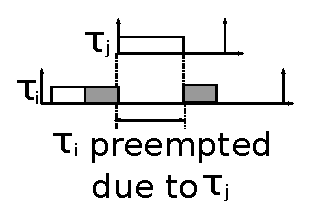
\includegraphics[scale=0.7]{figures/figure8}\caption{\label{fig8}Transactional retry due to release of higher priority
tasks}
\end{figure}
\end{comment}
\end{proof}

\begin{clm}\label{rcm rlease conflict}
Under RCM and G-RMA/LCM, the total retry cost suffered by all transactions in any $\tau_i^x$ during an interval $L\le T_i$ is upper bounded by:
\begin{equation}
RC_{to}(L)=RC(L)+RC_{re}(L)
\label{total rc rcm eq}
\end{equation}
%
where $RC(L)$ and $RC_{re}(L)$ are defined in Claim~\ref{ecm rlease conflict}. $RC(L)$ is calculated by (16) in~\cite{stmconcurrencycontrol:emsoft11} for RCM, and (8) in~\cite{lcmdac2012} for G-RMA/LCM. $RC_{re}(L)$ is calculated by:
\begin{equation}
RC_{re}(L)=\sum_{\forall \tau_j \in \zeta_i^*}\left(\left\lceil\frac{L}{T_j}\right\rceil s_{i_{max}}\right)\label{eq21}
\end{equation}
%
where $\zeta_i^*=\{\tau_j:p_j > p_i \}$.
\end{clm}
\begin{proof}\normalfont
The proof is the same as that for Claim~\ref{ecm rlease conflict}, except that G-RMA uses static priority. Thus, the carried-out jobs will be considered in the  interference with $\tau_i^x$. The carried-in jobs are still not considered because they are released before $r_i^x$. Claim follows.
\end{proof}
\begin{clm}\label{lock free release}
Consider lock-free synchronization. Let $r_{i_{max}}$ be the maximum execution cost of a single iteration of any retry loop of $\tau_i$. $RC_{re}$ under G-EDF  with lock-free synchronization is calculated by~(\ref{eq6}), where $s_{i_{max}}$ is replaced by $r_{i_{max}}$. $RC_{re}$ under G-RMA with lock-free synchronization is calculated by~(\ref{eq21}), where $s_{i_{max}}$ is replaced by $r_{i_{max}}$.
\end{clm}
%
\begin{proof}\normalfont
The interference pattern of higher priority jobs to lower priority jobs is the same in ECM, G-EDF/LCM, and G-EDF with lock-free. The pattern is also the same in RCM, G-RMA/LCM, and G-RMA with lock-free. 
%Claim follows.
\end{proof}


\subsection{PNF versus ECM\label{pnf vs ecm sec}}

\begin{clm}\label{PNF ecf comaprison clm}
In the absence of transitive retry, PNF/G-EDF's schedulability is better or equal to ECM's when conflicting atomic sections have equal lengths.
\end{clm}
\begin{proof}\normalfont
Substitue $RC_{A}(T_{i})$ and $RC_{B}(T_{i})$ in (\ref{utilization comparison})
with (\ref{rc-PNF}) and (\ref{total rc ecm eq}), respectively. Let $\theta_{i}^{ex}=\theta_{i}+\theta_{i}^{*}$, where $\theta_{i}^{*}$
is the set of objects not accessed directly by $\tau_{i}$ but can
cause transactions in $\tau_{i}$ to retry due to transitive retry.
Let $\gamma_{i}^{ex}=\gamma_{i}+\gamma_{i}^{*}$, where $\gamma_{i}^{*}$
is the set of tasks that access objects in $\theta_{i}^{*}$.
Let:
%
\begin{comment}
\begin{eqnarray*}
g(\tau_{i}) & = & \left(\sum_{\forall\tau_{j}\in\gamma_{i}^{*}}\sum_{\theta\in\theta_{i}^{*}}\left(\left\lceil \frac{T_{i}}{T_{j}}\right\rceil \sum_{\forall\bar{s_{j}^{k}(\theta)}}len\left(\bar{s_{j}^{k}(\theta)}\\
& + & s_{max}(\theta)\right)\right)\right) + RC_{re}(T_{i})
\end{eqnarray*}
\end{comment}
\begin{eqnarray*}
g(\tau_{i}) & = & \Bigg(\sum_{\forall\tau_{j}\in\gamma_{i}^{*}}\sum_{\theta\in\theta_{i}^{*}}\Bigg(\left\lceil \frac{T_{i}}{T_{j}}\right\rceil \sum_{\forall\bar{s_{j}^{k}(\theta)}}len\Big(\bar{s_{j}^{k}(\theta)}\\
 & + & s_{max}(\theta)\Big)\Bigg)\Bigg)+RC_{re}(T_{i})
\end{eqnarray*}
%
where $RC_{re}$ is given by~(\ref{eq6}). $g(\tau_i)$ includes effect of transitive retry. Let:
%
\begin{equation*}
\eta_{1}(\tau_{i})=\sum_{\forall\tau_{j}\in\gamma_{i}}\sum_{\forall\theta\in\theta_{i}}\left(\sum_{\bar{\forall s_{j}^{k}(\theta)}}len\left(\bar{s_{j}^{k}(\theta)}\right)\right)
\end{equation*}
%
\begin{equation*}
\eta_{2}(\tau_{i})=\sum_{\forall\tau_{j}\in\gamma_{i}}\sum_{\forall\theta\in\theta_{i}}\left(\left\lceil \frac{T_{i}}{T_{j}}\right\rceil \sum_{\forall\bar{s_{j}^{k}(\theta)}}len\left(s_{max}^{j}(\theta)\right)\right)
\end{equation*}
%
%and
%
\begin{equation*}
\eta_{3}(\tau_{i})=\sum_{\forall\tau_{j}\in\gamma_{i}}\sum_{\forall\theta\in\theta_{i}}\left(\left\lceil \frac{T_{i}}{T_{j}}\right\rceil \sum_{\bar{\forall s_{j}^{k}(\theta)}}len\left(\bar{s_{j}^{k}(\theta)}\right)\right)
\end{equation*}
%
By substitution of $g(\tau_{i})$, $\eta_1(\tau_i)$, and $\eta_2(\tau_i)$, and subtraction of $\sum_{\forall \tau_i} \frac{\eta_3(\tau_i)}{T_i}$ from both sides of (\ref{utilization comparison}), we get: 
\begin{equation}
\sum_{\forall \tau_i} \frac{\eta_1(\tau_i)}{T_i} \le \sum_{\forall \tau_i} \frac{\eta_2(\tau_i)+g(\tau_i)}{T_i}
\label{PNF ecm comparison 2}
\end{equation}
Assume that $g(\tau_{i})_{\forall\tau_{i}}\rightarrow0$. From (\ref{PNF ecm comparison 2}), we note that by keeping
every $len(\bar{s_{j}^{k}(\theta)})\le len(s_{max}^{j}(\theta))$
for each $\tau_{i}$, $\tau_{j}\in\gamma_{i}$, and $\theta\in\theta_{i}$,  (\ref{PNF ecm comparison 2}) holds. 
%
Due to G-EDF's dynamic priority, $s_{max}^{j}(\theta)$
can belong to any task other than $\tau_{j}$. By keeping $len(\bar{s_j^k(\theta)})\le len(s_{max}^j(\theta))$, then~\ref{PNF ecm comparison 2} holds. By generalizing this condition to any $s_j^k(\theta)$ and $s_{max}^j(\theta)$, then~\ref{PNF ecm comparison 2} holds if all atomic sections in all tasks have equal lengths. Claim follows.
\end{proof}

\subsection{PNF versus RCM}\label{pnf vs rcm sec}

\begin{clm}\label{clm_pnf_rcm_comp}
In the absence of transitive retry, PNF/G-RMA's schedulability is better or equal to RCM's schedulability when a large number of tasks heavily conflict. PNF's schedulability is improved compared with RCM's, when atomic section length increases as priority increases. 
\end{clm}
\begin{proof}\normalfont
Let $\theta_{i}^{ex}=\theta_{i}+\theta_{i}^{*}$ and $\gamma_{i}^{ex}=\gamma_{i}+\gamma_{i}^{*}$, as defined in the proof of Claim~\ref{PNF ecf comaprison clm}. Substitute $RC_{A}(T_{i})$ and $RC_{B}(T_{i})$ in (\ref{utilization comparison}) with (\ref{rc-PNF}) and (\ref{total rc rcm eq}), respectively. Let: 
% 
\begin{eqnarray*}
g(\tau_{i}) & =RC_{re}(T_{i})+\Bigg( & \sum_{\forall\tau_{j}\in(\gamma_{i}^{*}\cap\zeta_{i}^{*})}\sum_{\forall\theta\in\theta_{i}^{*}}\left(\left\lceil \frac{T_{i}}{T_{j}}\right\rceil +1\right)\times\\
 &  & \sum_{\forall\bar{s_{j}^{k}(\theta)}}len\left(\bar{s_{j}^{k}(\theta)}+s_{max}^{j}(\theta)\right)\Bigg)
\end{eqnarray*}
%
where $RC_{re}$ and $\zeta_i^*$ are defined by~(\ref{eq21}). $g(\tau_i)$ includes effect of transitive retry. 
Let $\gamma_{i}=\zeta_{i}^{*}\cup\bar{\zeta_{i}}$, where $\bar{\zeta_{i}}=\left\{ \tau_{j}:\left(\tau_{j}\ne\tau_{i}\right)\wedge\left(p_{j}<p_{i}\right)\right\} $,
thus $\zeta_{i}^{*}\cap\bar{\zeta_{i}}=\phi$.

Let:
%
\begin{equation*}
\eta_{1}(\tau_{i})=\sum_{\forall\tau_{j}\in(\gamma_{i}\cap\zeta_{i}^{*})}\sum_{\forall\theta\in\theta_{i}}\left(\left(\left\lceil \frac{T_{i}}{T_{j}}\right\rceil +1\right)\sum_{\bar{\forall s_{j}^{k}(\theta)}}len\left(\bar{s_{j}^{k}(\theta)}\right)\right)
\end{equation*}
%
\begin{equation*}
\eta_{2}(\tau_{i})=\sum_{\forall\tau_{j}\in(\gamma_{i}\cap\bar{\zeta_{i}})}\sum_{\forall\theta\in\theta_{i}}\left(\left(\left\lceil \frac{T_{i}}{T_{j}}\right\rceil +1\right)\sum_{\bar{\forall s_{j}^{k}(\theta)}}len\left(\bar{s_{j}^{k}(\theta)}\right)\right)
\end{equation*}
%
%and
%
\begin{eqnarray*}
\eta_{3}(\tau_{i}) & = & \sum_{\forall\tau_{j}\in(\gamma_{i}\cap\zeta_{i}^{*})}\sum_{\forall\theta\in\theta_{i}}\Bigg(\left(\left\lceil \frac{T_{i}}{T_{j}}\right\rceil +1\right)\times\\
 &  & \sum_{\forall\bar{s_{j}^{k}(\theta)}}len\left(\bar{s_{j}^{k}(\theta)}+s_{max}^{j}(\theta)\right)\Bigg)
\end{eqnarray*}
%
By substitution of $g(\tau_i)$, $\eta_1(\tau_i)$, $\eta_2(\tau_i)$, and $\eta_3(\tau_i)$ in (\ref{utilization comparison}):
%
\begin{equation}
\sum_{\forall\tau_{i}}\frac{\eta_{1}(\tau_{i})+\eta_{2}(\tau_{i})}{T_{i}}\le\sum_{\forall\tau_{i}}\frac{\eta_{3}(\tau_{i})+g(\tau_{i})}{T_{i}}
\label{PNF rcm comparison 3}
\end{equation}
%
When tasks with deadlines equal to periods are scheduled with G-RMA, $T_{j}>T_{i}$ if $p_{j}<p_{i}$. So, for each $\tau_{j}\in\bar{\zeta_{i}}$, $\left\lceil \frac{T_{i}}{T_{j}}\right\rceil =1$. Then:
%
\begin{equation}
\eta_{2}(\tau_{i})=2\sum_{\forall\tau_{j}\in(\gamma_{i}\cap\bar{\zeta_{i}})}\sum_{\forall\theta\in\theta_{i}}\sum_{\bar{\forall s_{j}^{k}(\theta)}}len\left(\bar{s_{j}^{k}(\theta)}\right)
\label{PNF rcm comparison 5}
\end{equation}
%
Let:
%
\begin{equation*}
\eta_{4}(\tau_{i})=\sum_{\forall\tau_{j}\in(\gamma_{i}\cap\zeta_{i}^{*})}\sum_{\forall\theta\in\theta_{i}}\left(\left\lceil \frac{T_{i}}{T_{j}}\right\rceil +1\right)\sum_{\forall\bar{s_{j}^{k}(\theta)}}len\left(s_{max}^{j}(\theta)\right)
\end{equation*}
%
By substitution of~(\ref{PNF rcm comparison 5}) and subtraction of $\sum_{\forall \tau_i} \frac{\eta_1 (\tau_i)}{T_i}$ from both sides of~(\ref{PNF rcm comparison 3}), we get:
%
\begin{equation}
2\sum_{\forall\tau_{i}}\frac{\eta_{2}(\tau_{i})}{T_{i}}\le\sum_{\forall\tau_{i}}\frac{\eta_{4}(\tau_{i})+g(\tau_{i})}{T_{i}}
\label{PNF rcm comparison 4}
\end{equation}
%
Assume that $g(\tau_{i})_{\forall\tau_{i}}\rightarrow0$. From (\ref{PNF rcm comparison 4}), we note that when higher priority jobs increasingly conflict with lower priority jobs, (\ref{PNF rcm comparison 4}) tends to hold. (\ref{PNF rcm comparison 4}) also tends to hold if $len(\bar{s_{max}^j(\theta)})$ in the right hand side of (\ref{PNF rcm comparison 4}) is larger than $len(\bar{s_j^k(\theta)})$ in the left hand side of (\ref{PNF rcm comparison 4}), which means atomic section length increases as priority increases. Claim follows.
\end{proof}

\subsection{PNF versus G-EDF/LCM}

\begin{clm}\label{sub:pnf_lcm_edf_comp}
In the absence of transitive retry, PNF/EDF's schedulability is equal or better than G-EDF/LCM's if the conflicting atomic section lengths are approximately equal and all $\alpha$ terms approach 1.

\end{clm}
\begin{proof}\normalfont
Assume that $\eta_{1}(\tau_i)$ and $\eta_{3}(\tau_i)$ are the same as that defined in the proof
of Claim~\ref{PNF ecf comaprison clm}. Let:
\begin{eqnarray*}
g(\tau_{i}) & = & \Bigg(\sum_{\forall\tau_{j}\in\gamma_{i}^{*}}\sum_{\theta\in\theta_{i}^{*}}\Bigg(\left\lceil \frac{T_{i}}{T_{j}}\right\rceil \sum_{\forall\bar{s_{j}^{k}(\theta)}}len\Big(\bar{s_{j}^{k}(\theta)}\\
 & + & \alpha_{max}^{ji}s_{max}(\theta)\Big)\Bigg)\Bigg)+RC_{re}(T_{i})
\end{eqnarray*}
\[
\eta_{2}(\tau_{i})=\sum_{\forall\tau_{j}\in\gamma_{i}}\sum_{\forall\theta\in\theta_{i}}\left(\left\lceil \frac{T_{i}}{T_{j}}\right\rceil \sum_{\forall\bar{s_{j}^{k}(\theta)}}len\left(\alpha_{max}^{jl}s_{max}^{j}(\theta)\right)\right)
\]
where $\alpha_{max}^{jl}$ is defined in~(\ref{eq78}). Following the same steps in the proof of Claim~\ref{PNF ecf comaprison clm}, we get:
\begin{equation}
\sum_{\forall\tau_{i}}\frac{\eta_{1}(\tau_{i})}{T_{i}}\le\sum_{\forall\tau_{i}}\frac{\eta_{2}(\tau_{i})+g(\tau_{i})}{T_{i}}\label{eq:pnf_lcm_edf_comp}
\end{equation}
Assume that $g(\tau_{i})_{\forall\tau_{i}}\rightarrow0$. Thus, we ignore the effect of transitive retry and retry cost due to the release of higher priority jobs. Let $len(\bar{s_{j}^{k}(\theta)})=s_{max}^{j}(\theta)=s$,
and $\alpha_{max}^{jl}=\alpha_{max}^{iy}=1$ in (\ref{eq:pnf_lcm_edf_comp}). Then, PNF/EDF's schedulability equals LCM/EDF's schedulability if
$\left\lceil \frac{T_{i}}{T_{j}}\right\rceil =1,\,\forall\tau_{i},\tau_{j}$
(which means equal periods for all tasks). If $\left\lceil \frac{T_{i}}{T_{j}}\right\rceil >1,\,\forall\tau_{i},\tau_{j}$,
PNF/EDF's schedulability is better than LCM/EDF's. PNF/EDF's schedulability  becomes more better than LCM/EDF's schedulability if $g(\tau_{i})$
is not zero. Claim follows.
\end{proof}

%\begin{comment}
\subsection{PNF versus G-RMA/LCM}

\begin{clm}\label{sub:pnf_lcm_rma_comp}
%
In the absence of transitive retry, PNF's schedulability is equal or better than G-RMA/LCM's if: 1) lower priority tasks suffer increasing number of conflicts from higher priority tasks, 2) the lengths of the atomic sections increase as task priorities increase, and 3) $\alpha$ terms increase.
%
\end{clm}
\begin{proof}\normalfont
Assume that $g(\tau_{i})$, $\eta_{1}(\tau_{i})$, and $\eta_{2}(\tau_{i})$ are the same as in the proof of Claim~\ref{clm_pnf_rcm_comp}. Let:
\begin{eqnarray*}
\eta_{3}(\tau_{i}) & = & \sum_{\forall\tau_{j}\in(\gamma_{i}\cap\zeta_{i}^{*})}\sum_{\forall\theta\in\theta_{i}}\Bigg(\left(\left\lceil \frac{T_{i}}{T_{j}}\right\rceil +1\right)\times\\
 &  & \sum_{\forall\bar{s_{j}^{k}(\theta)}}len\left(\bar{s_{j}^{k}(\theta)}+\alpha_{max}^{jl}s_{max}^{j}(\theta)\right)\Bigg)
\end{eqnarray*}
%and
\begin{eqnarray*}
\eta_{4}(\tau_{i}) & = & \sum_{\forall\tau_{j}\in(\gamma_{i}\cap\zeta_{i}^{*})}\sum_{\forall\theta\in\theta_{i}}\Bigg(\left(\left\lceil \frac{T_{i}}{T_{j}}\right\rceil +1\right)\\
 & \times & \sum_{\forall\bar{s_{j}^{k}(\theta)}}len\left(\alpha_{max}^{jl}s_{max}^{j}(\theta)\right)\Bigg)
\end{eqnarray*}
Following the steps of Claim~\ref{clm_pnf_rcm_comp}'s proof, 
$\therefore$(\ref{utilization comparison}) becomes:
\begin{equation}
2\sum_{\forall\tau_{i}}\frac{\eta_{2}(\tau_{i})}{T_{i}}\le\sum_{\forall\tau_{i}}\frac{\eta_{4}(\tau_{i})+g(\tau_{i})}{T_{i}}\label{pnf-lcm-rma-comp-2}
\end{equation}
Assume that the effect of transitive retry and retry cost due
to the release of higher priority jobs is negligible ($g(\tau_{i})\rightarrow0$). (\ref{pnf-lcm-rma-comp-2})
holds if: 1) the contention from higher priority jobs to lower priority
jobs increases because of the $\left\lceil \frac{T_{i}}{T_{j}}\right\rceil +1$
term in the right hand side of (\ref{pnf-lcm-rma-comp-2}); 2) $\alpha$ terms
approach 1; and 3) the lengths of the atomic sections increase as priority
increases. 
%
This makes $len(s_{max}^{j}(\theta))$ in (\ref{pnf-lcm-rma-comp-2})'s right 
side to be greater than $len(\bar{s_{j}^{k}(\theta)})$ in (\ref{pnf-lcm-rma-comp-2})'s left  side.
Claim follows.
\end{proof}
%\end{comment}

\subsection{PNF versus Lock-free Synchronization\label{pnf vs lock free sec}}

Lock-free synchronization~\cite{key-5,stmconcurrencycontrol:emsoft11} accesses only one object. Thus, the number of accessed objects per transaction in PNF is limited to one. This allows us to compare the schedulability of PNF with the lock-free algorithm. 

$RC_{B}(T_{i})$ in (\ref{utilization comparison}) is replaced with:
%
\begin{equation}
\sum_{\forall\tau_{j}\in\gamma_{i}}\Bigg(\left(\left\lceil \frac{T_{i}}{T_{j}}\right\rceil +1\right)\beta_{i,j}r_{max}\Bigg)+RC_{re}(T_{i})
\label{lock-free rc}
\end{equation}
%
where $\beta_{i,j}$ is the number of retry loops of $\tau_{j}$ that access the same object as accessed by some retry loop of $\tau_{i}$~\cite{key-5}. $r_{max}$ is the maximum execution cost of a single iteration of any retry loop of any task~\cite{key-5}. $RC_{re}(T_i)$ is defined in Claim~\ref{lock free release}. Lock-free synchronization does not depend on priorities  of tasks. Thus,~(\ref{lock-free rc}) applies for both G-EDF and G-RMA systems.


%%
\begin{clm}\label{PNF lock-free comparison}
Let $r_{max}$ be the maximum execution cost of a single iteration of any retry loop of any task~\cite{key-5}. Let $s_{max}$ be the maximum transaction length in all tasks. Assume that each transaction under PNF accesses only one object for once. The schedulability of PNF with either G-EDF or G-RMA scheduler is better or equal to the schedulability of lock-free
synchronization if $s_{max}/r_{max}\le 1$.
\end{clm}
\begin{proof}\normalfont
The assumption in Claim~\ref{PNF lock-free comparison} is made to enable a comparison between PNF and lock-free. Let $RC_{A}(T_{i})$ in (\ref{utilization comparison}) be replaced
with (\ref{rc-PNF}) and $RC_{B}(T_{i})$ be replaced with (\ref{lock-free rc}).
To simplify comparison, (\ref{rc-PNF}) is upper bounded by:
%
\begin{equation*}
RC(T_{i})=\sum_{\tau_{j}\in\gamma_{i}}\left(\left(\left\lceil \frac{T_{i}}{T_{j}}\right\rceil +1\right)\beta_{i,j}^* s_{max}\right)
\end{equation*}
%
where $\beta_{i,j}^*$ is the number of times transactions in $\tau_j$ accesses shared objects with $
\tau_i$. Thus, $\beta_{i,j}^* = \beta_{i,j}$, and (\ref{utilization comparison}) will be:
\begin{eqnarray}
\sum_{\forall\tau_{i}}\frac{\sum_{\tau_{j}\in\gamma_{i}}\left(\left(\left\lceil \frac{T_{i}}{T_{j}}\right\rceil +1\right)\beta_{i,j}s_{max}\right)}{T_{i}} & \le\nonumber \\
\sum_{\forall\tau_{i}}\frac{\sum_{\forall\tau_{j}\in\gamma_{i}}\left(\left\lceil \frac{T_{i}}{T_{j}}\right\rceil +1\right)\beta_{i,j}r_{max}+RC_{re}(\tau_i)}{T_{i}}\label{eq:PNF lock-free comparison}
\end{eqnarray}
From (\ref{eq:PNF lock-free comparison}), we note that if $s_{max}\le r_{max}$,
then (\ref{eq:PNF lock-free comparison}) holds. 
%Claim follows.
\end{proof}

\section{First Bounded, Last Timestamp CM (FBLT)}
With PNF, all objects accessed by each transaction must be known a-priori. Therefore, this is not suitable with dynamic STM implementations~\cite{Herlihy:2003:STM:872035.872048}. Additionally, PNF is implemented in~\cite{shambake_phd_proposal} as a centralized CM that uses locks. This increases overhead. 

\subsection{Case for FBLT}

It is desirable to have a CM with the following goals:
\begin{compactenum}
\item \label{goal 1} reduce the retry cost of each transaction $s_i^k$ due to another transaction $s_j^l$, just as LCM does compared to ECM and RCM.
\item \label{goal 2} avoid or bound the effect of transitive retry, similar to PNF, without prior knowledge of accessed objects by each transaction, enabling dynamic STM.
\item \label{goal 3} decentralized design and avoid the use of locks, thereby reducing  overhead.
\end{compactenum}

We propose the \textit{First Bounded, Last Timestamp contention manager} (or (FBLT). FBLT achieves these goals by bounding the number of times each transaction $s_i^k$ is aborted due to other transactions to at most $\delta_i^k$. $\delta_i^k$ includes the number of aborts due to direct conflict with other transactions, as well as transitive retry (goal~\ref{goal 2}). If a transaction $s_i^k$ reaches its $\delta_i^k$, it is added to an $m\_$set in FIFO order. In the $m\_$set, $s_i^k$ executes non-preemptively. If transactions in the $m\_$set conflict together, they use their FIFO order in the $m\_$set to resolve the conflict. $s_i^k$ can still abort after it becomes a non-preemptive transaction due to other non-preemptive transactions. The number of aborts for any non-preemptive transaction is bounded by $m-1$ , where $m$ is the number of processors, as will be shown in Section~\ref{fblt rc}. 

Thus, the key idea behind FBLT is to use a suitable $\delta_i^k$ for each $s_i^k$ before it becomes a non-preemptive transaction. The choice of $\delta_i^k$ should make the total retry cost (and thus, the schedulability) of any job $\tau_i^x$ under FBLT comparable to the retry cost under ECM, RCM, LCM, and PNF. (In Section~\ref{schedulabiltiy comparison}, we show the suitable $\delta_i^k$ for each $s_i^k$ to have equal or better schedulability than other CMs.) Preemptive transactions resolve their conflicts using LCM.  Thus, FBLT defaults to LCM if abort bounds have not been violated (goal~\ref{goal 1}). Each non-preemptive transaction $s_i^k$  uses the time it joined the $m\_$set to resolve conflicts with other non-preemptive transactions. Therefore, FBLT does not have to use locks and is decentralized (goal~\ref{goal 3}).


\section{The FBLT Contention Manager}
\label{sec:fblt design}

\begin{algorithm}[h!]
\footnotesize{
\LinesNumbered
\KwData{
$s_i^k$: interfered transaction\;
$s_j^l$: interfering transactions\;
$\delta_i^k$: the maximum number of times $s_i^k$ can be aborted during $T_i$\;
$\eta_i^k$: number of times $s_i^k$ has already been aborted up to now\;
$m\_$set: contains at most $m$ non-preemptive transactions. $m$ is number of processors\;
$m\_prio$: priority of any transaction in $m\_$set. $m\_prio$ is higher than any priority of any real-time task\;
$r(s_i^k)$: time point at which $s_i^k$ joined $m\_$set\;
}
\KwResult{atomic sections that will abort}
\uIf{\label{both preemptive}$s_i^k,\,s_j^l \not\in m\_set$}
{
Apply Algorithm~\ref{alg_lcm} (default to LCM)\label{apply lcm}\;
\eIf{\label{preemptive s_i^k aborted}$s_i^k$ is aborted}
{
\eIf{$\eta_i^k<\delta_i^k$}
{
Increment $\eta_i^k$ by 1\label{increment eta 1}\;
}
{
Add $s_i^k$ to $m\_$set\label{add to m_set 1}\;
Record $r(s_i^k)$\label{record 1}\;
Increase priority of $s_i^k$ to $m\_prio$\label{increase priority 1}\;
}
}
{
Swap $s_i^k$ and $s_j^l$\;
Go to Step~\ref{preemptive s_i^k aborted}\;
}
}
\uElseIf{\label{s_j^l is non preemptive}$s_j^l \in m\_set,s_i^k \not\in m\_set$}
{
Abort $s_i^k$\;
\eIf{$\eta_i^k < \delta_i^k$}
{
Increment $\eta_i^k$ by 1\label{increment eta 2}\;
}
{
Add $s_i^k$ to $m\_$set\label{add to m_set 2}\;
Record $r(s_i^k)$\label{record 2}\;
Increase priority of $s_i^k$ to $m\_prio$\label{increase priority 2}\;
}
}
\uElseIf{\label{s_i^k is non-preemptive}$s_i^k \in m\_set,s_j^l \not\in m\_set$}
{
Swap $s_i^k$ and $s_j^l$\;
Go to Step~\ref{s_j^l is non preemptive}\label{end preemptive and non preemptive}\;
}
\Else
{
\label{both non preemptive}
\eIf{$r(s_i^k)<r(s_j^l)$}
{	
Abort $s_j^l$\label{s_i^k first in m_set}\;
}
{
Abort $s_i^k$\label{s_j^l first in m_set}\;
}
}
}
\caption{The FBLT Algorithm}\label{fblt-algorithm}
\end{algorithm}

Algorithm~\ref{fblt-algorithm} illustrates FBLT. Each transaction $s_{i}^{k}$ can be aborted during $T_i$ for at most $\delta_{i}^{k}$ times. $\eta_{i}^{k}$ records  the number of times $s_{i}^{k}$ has already been aborted up to now. If $s_i^k$ and $s_j^l$ have not joined the $m\_$set yet, then they are preemptive transactions. Preemptive transactions resolve conflicts using Algorithm~\ref{alg_lcm} (step~\ref{apply lcm}). Thus, FBLT defaults to LCM when no transaction reaches its $\delta$. If only one of the transactions is in the $m\_$set, then the non-preemptive transaction (the one in $m\_$set) aborts the other one (steps~\ref{s_j^l is non preemptive} to~\ref{end preemptive and non preemptive}). $\eta_i^k$ is incremented each time $s_i^k$ is aborted as long as $\eta_i^k < \delta_i^k$ (steps~\ref{increment eta 1} and~\ref{increment eta 2}). Otherwise, $s_i^k$ is added to the $m\_$ set and its priority is increased to $m\_prio$ (steps~\ref{add to m_set 1} to~\ref{increase priority 1} and~\ref{add to m_set 2} to~\ref{increase priority 2}). When the priority of $s_i^k$ is increased to $m\_prio$, $s_i^k$ becomes a non-preemptive transaction. Non-preemptive transactions cannot be aborted by other preemptive transactions, nor by any other real-time job. The $m\_$set can hold at most $m$ concurrent transactions because there are $m$ processors in the system. $r(s_i^k)$ records the time $s_i^k$ joined the $m\_$set (steps~\ref{record 1} and~\ref{record 2}). When non-preemptive transactions conflict together (step~\ref{both non preemptive}), the transaction with the smaller $r()$ commits first (steps~\ref{s_i^k first in m_set} and~\ref{s_j^l first in m_set}). Thus, non-preemptive transactions are executed in FIFO order of the $m\_$set.

\subsection{Illustrative Example}

We now illustrate FBLT's behavior with the following example:
\begin{compactenum}
\item Transaction $s_{i}^{k}(\theta_{1},\theta_{2})$ is released while
$m\_set=\emptyset$. $\eta_{i}^{k}=0$ and $\delta_{i}^{k}=3$.
\item \label{fblt_ex_step 2} Transaction $s_{a}^{b}(\theta_{2})$ is released
while $s_{i}^{k}(\theta_{1},\theta_{2})$ is running. $p_{a}^{b}>p_{i}^{k}$
and $\eta_{i}^{k}<\delta_{i}^{k}$. Applying LCM, $s_{i}^{k}(\theta_{1},\theta_{2})$
is aborted in favor of $s_{a}^{b}$ and $\eta_{i}^{k}$ is incremented
to 1.
\item $s_{a}^{b}(\theta_{2})$ commits. $s_{i}^{k}(\theta_{1},\theta_{2})$
runs again. Transaction $s_{c}^{d}(\theta_{2})$ is released while
$s_{i}^{k}(\theta_{1},\theta_{2})$ is running. $p_{c}^{d}>p_{i}^{k}$. Applying LCM, $s_{i}^{k}(\theta_{1},\theta_{2})$ is aborted again in favor of $s_{c}^{d}(\theta_{2})$.
$\eta_{i}^{k}$ is incremented to 2.
\item $s_{c}^{d}(\theta_{2})$ commits. $s_{e}^{f}(\theta_{2},\theta_{3})$
is released. $p_{e}^{f}>p_{i}^{k}$ and $\eta_{e}^{f}=2$. $s_{i}^{k}(\theta_{1},\theta_{2})$
is aborted in favor of $s_{e}^{f}(\theta_{2},\theta_{3})$ and $\eta_{i}^{k}$
is incremented to 3.
\item $s_{j}^{l}(\theta_{3})$ is released. $p_{j}^{l}>p_{e}^{f}$. $s_{e}^{f}(\theta_{2},\theta_{3})$ is aborted in favor of $s_{j}^{l}(\theta_{3})$
and $\eta_{e}^{f}$ is incremented to 1.
\item \label{fblt_ex_step 6} $s_{i}^{k}(\theta_{1},\theta_{2})$ and $s_{e}^{f}(\theta_{2},\theta_{3})$
are compared again. $\because\,\eta_{i}^{k}=\delta_{i}^{k}$, $\therefore\, s_{i}^{k}(\theta_{1},\theta_{2})$
is added to $m\_$set. $m\_set=\left\{ s_{i}^{k}(\theta_{1},\theta_{2})\right\} $.
$s_{i}^{k}(\theta_{1},\theta_{2})$ becomes a non-preemptive transaction.
As $s_{e}^{f}(\theta_{2},\theta_{3})$ is a preemptive transaction, $\therefore\, s_{e}^{f}(\theta_{2},\theta_{3})$ is aborted in
favor of $s_{i}^{k}(\theta_{1},\theta_{2})$, despite $p_{e}^{f}$ being greater than the original priority of $s_i^k(\theta_1,\theta_2)$. $\eta_{e}^{f}$ is incremented to 2.
%
\item \label{fblt_ex_step 7} $s_{j}^{l}(\theta_{3})$ commits but $s_{g}^{h}(\theta_{3})$
is released. $p_{g}^{h}>p_{e}^{f}$ but $\eta_{e}^{f}=\delta_{e}^{f}$.
So, $s_{e}^{f}(\theta_{2},\theta_{3})$ becomes a non-preemptive transaction.
$m\_set=\left\{ s_{i}^{k}(\theta_{1},\theta_{2}),s_{g}^{h}(\theta_{2},\theta_{3})\right\} $.
%
\item $s_{i}^{k}(\theta_{1},\theta_{2})$ and $s_{g}^{h}(\theta_{2},\theta_{3})$
are now non-preemptive transactions. $s_{i}^{k}(\theta_{1},\theta_{2})$
and $s_{g}^{h}(\theta_{2},\theta_{3})$ still conflict together. So,
they are executed according to their addition order to the $m\_$set.
So, $s_{i}^{k}(\theta_{1},\theta_{2})$ commits first, followed $s_{g}^{h}(\theta_{2},\theta_{3})$.
\item $s_{g}^{h}(\theta_{3})$ will continue to abort and retry in favor
of $s_{e}^{f}(\theta_{2},\theta_{3})$ until $s_{e}^{f}(\theta_{2},\theta_{3})$
commits or $\eta_{g}^{h}=\delta_{g}^{h}$. Even if $s_{g}^{h}(\theta_{3})$
joined the $m\_$set, $s_{g}^{h}(\theta_{3})$ will still abort and retry
in favor of $s_{e}^{f}(\theta_{2},\theta_{3})$, because $s_{e}^{f}(\theta_{2},\theta_{3})$ joined the $m\_$set earlier than $s_{g}^{h}(\theta_{3})$.
\end{compactenum}

It is seen from steps \ref{fblt_ex_step 2} to \ref{fblt_ex_step 6}
that $s_{i}^{k}(\theta_{1},\theta_{2})$ can be aborted due to direct
conflict with other transactions, or due to transitive retry. Irrespective of 
the reason for the conflict, once a transaction has reached its maximum
allowed $\delta$, the transaction becomes a non-preemptive one
(steps \ref{fblt_ex_step 6} and \ref{fblt_ex_step 7}). Non-preemptive
transactions have higher priority than other preemptive transactions
(steps \ref{fblt_ex_step 6} and \ref{fblt_ex_step 7}). Non-preemptive
transactions execute in their arrival order to the $m\_$set.


\section{Retry Cost and Response Time Bounds}\label{fblt rc}

We now derive an upper bound on the retry cost of any job $\tau_{i}^{x}$
under FBLT during an interval $L\le T_{i}$. Since all tasks are sporadic
(i.e., each task $\tau_{i}$ has a minimum period $T_{i}$), $T_{i}$
is the maximum study interval for each task $\tau_{i}$.

\begin{clm}
The total retry cost for any job $\tau_{i}^{x}$ under FBLT due to 1) conflicts
between its transactions and transactions of other jobs during an interval $L\le T_{i}$ and 2) release of higher priority jobs is upper bounded by:
%
\begin{equation}
RC_{to}(L)\le\sum_{\forall s_{i}^{k}\in s_{i}}\left(\delta_{i}^{k}len(s_{i}^{k})+\sum_{\forall s_{iz}^k\in \chi_i^k} len(s_{iz}^{k})\right)+RC_{re}(L)\label{eq:fblt_rc}
\end{equation} 
where $\chi_i^k$ is the set of at most $m-1$ maximum length transactions conflicting directly or indirectly (through transitive retry) with $s_i^k$. Each transaction $s_{iz}^k \in \chi_i^k$ belongs to a distinct task $\tau_j$. $RC_{re}(L)$ is the retry cost resulting
from the release of higher priority jobs which preempt $\tau_{i}^{x}$.
$RC_{re}(L)$ is calculated by (6.8) in \cite{shambake_phd_proposal}
for G-EDF, and (6.10) in \cite{shambake_phd_proposal} for G-RMA schedulers.
%
\end{clm}


\begin{proof}\normalfont
By the definition of FBLT, $s_{i}^{k}\in\tau_{i}^{x}$ can be aborted
a maximum of $\delta_{i}^{k}$ times before $s_{i}^{k}$ joins the $m\_$set. Before joining the $m\_$set, $s_{i}^{k}$ can be aborted due to higher priority transactions, or transactions
in the $m\_$set. The original priority of transactions in the $m\_$set can be higher or lower than
$p_{i}^{x}$. Thus, the maximum time $s_{i}^{k}$ is aborted before
joining the $m\_$set occurs if $s_{i}^{k}$ is aborted for $\delta_{i}^{k}$ times. 

Transactions preceding  $s_i^k$ in the $m\_$set can conflict directly with $s_i^k$, or indirectly through transitive retry. The worst case scenario for $s_{i}^{k}$ after joining the $m\_$set occurs if $s_{i}^{k}$ is preceded by $m-1$ maximum length conflicting transactions. Hence, in the worst case, $s_{i}^{k}$ has to wait for the previous $m-1$ transactions to commit first. The priority of $s_{i}^{k}$ after joining the $m\_$set is higher than any real-time job. Therefore, $s_{i}^{k}$ is not aborted
by any job. If $s_{i}^{k}$ has not joined the $m\_$ set yet, and a higher
priority job $\tau_{j}^{y}$ is released while $s_{i}^{k}$ is running,
then $s_{i}^{k}$ may be aborted if $\tau_{j}^{y}$ has conflicting
transactions with $s_{i}^{k}$. $\tau_{j}^{y}$ causes only one abort
in $\tau_{i}^{x}$ because $\tau_{j}^{y}$ preempts $\tau_{i}^{x}$
only once. If $s_{i}^{k}$ has already joined the $m\_$set, then $s_{i}^{k}$
cannot be aborted by the release of higher priority jobs. Thus, the maximum
number of times transactions in $\tau_{i}^{x}$ can be aborted due to the release
of higher priority jobs is less than or equal to the number of interfering
higher priority jobs to $\tau_{i}^{x}$. Claim follows.
\end{proof}

\begin{clm}
Under FBLT, the blocking time of a job $\tau_{i}^{x}$ due to lower priority
jobs is upper bounded by: 
\begin{equation}
D(\tau_{i}^{x})=min\left(max_{1}^{m}(s_{j_{max},\forall\tau_{j}^{l},\, p_{j}^{l}<p_{i}^{x}})\right)\label{eq:fblt_delay}
\end{equation}
where $s_{j_{max}}$ is the maximum length transaction in any job
$\tau_{j}^{l}$ with original priority lower than $p_{i}^{x}$. The
right hand side of (\ref{eq:fblt_delay}) is the minimum of the $m$
maximum transactional lengths in all jobs with lower priority than
$\tau_{i}^{x}$.
\end{clm}


\begin{proof}\normalfont
$\tau_{i}^{x}$ is blocked when it is initially released and all processors
are busy with lower priority jobs with non-preemptive transactions.
Although $\tau_{i}^{x}$ can be preempted by higher priority jobs,
$\tau_{i}^{x}$ cannot be blocked after it is released. If $\tau_{i}^{x}$
is preempted by a higher priority job $\tau_{j}^{y}$, then, when $\tau_{j}^{y}$
finishes execution, the underlying scheduler will not choose a lower
priority job than $\tau_{i}^{x}$ before $\tau_{i}^{x}$. So, after
$\tau_{i}^{x}$ is released, there is no chance for any transaction
$s_{u}^{v}$ belonging to a lower priority job than $\tau_{i}^{x}$
to run before $\tau_{i}^{x}$. Thus, $s_{u}^{v}$ cannot join the $m\_$set
before $\tau_{i}^{x}$ finishes. Consequently, the worst case blocking
time for $\tau_{i}^{x}$ occurs when the maximum length $m$ transactions
in lower priority jobs than $\tau_{i}^{x}$ are executing non-preemptively.
After the minimum length transaction in the $m\_$set finishes, the
underlying scheduler will choose $\tau_{i}^{x}$ or a higher priority
job to run. Claim follows.
\end{proof}

\begin{clm}
The response time of any job $\tau_{i}^{x}$ during an interval $L\le T_{i}$
under FBLT is upper bounded by:
\begin{equation}
R_{i}^{up}=c_{i}+RC_{to}(L)+D(\tau_{i}^{x})+\left\lfloor \frac{1}{m}\sum_{\forall j\ne i}W_{ij}(R_{i}^{up})\right\rfloor \label{eq:fblt_res_time}
\end{equation}
where $RC_{to}(L)$ is calculated by (\ref{eq:fblt_rc}), $D(\tau_{i}^{x})$
is calculated by (\ref{eq:fblt_delay}), and $W_{ij}(R_{i}^{up})$
is calculated by (11) in \cite{stmconcurrencycontrol:emsoft11} for
G-EDF, and (17) in \cite{stmconcurrencycontrol:emsoft11} for G-RMA schedulers.
(11) and (17) in \cite{stmconcurrencycontrol:emsoft11} inflates $c_{j}$
of any job $\tau_{j}^y\ne\tau_{i}^x,\, p_{j}^y>p_{i}^x$ by the retry cost
of transactions in $\tau_{j}^y$.
\end{clm}


\begin{proof}\normalfont
The response time of a job is calculated directly from FBLT's behavior. The response time of any job $\tau_{i}^{x}$ is the sum of its
worst case execution time $c_{i}$, plus the retry cost of transactions
in $\tau_{i}^{x}$ ($RC_{to}(L)$), plus the blocking time of $\tau_{i}^{x}$
($D(\tau_{i}^{x})$), and the workload interference of higher priority
jobs. The workload interference of higher priority jobs scheduled by
G-EDF is calculated by (11) in \cite{stmconcurrencycontrol:emsoft11},
and by (17) in \cite{stmconcurrencycontrol:emsoft11} for G-RMA. Claim follows.
\end{proof}

\begin{comment}
We now derive an upper bound on the retry cost of any job $\tau_{i}^{x}$
under FBLT during an interval $L\le T_{i}$. Since all tasks are sporadic
(i.e., each task $\tau_{i}$ has a minimum period $T_{i}$), $T_{i}$
is the maximum study interval for each task $\tau_{i}$.

\begin{clm}

The total retry cost for any job $\tau_{i}^{x}$ under FBLT due to: 1) conflicts
between its transactions and transactions of other jobs during an interval $L\le T_{i}$. 2) release of higher priority jobs, is upper bounded by:

\begin{equation}
RC_{to}(L)\le\sum_{\forall s_{i}^{k}\in s_{i}}\left(\delta_{i}^{k}len(s_{i}^{k})+\sum_{\forall s_{iz}^k\in \chi_i^k} len(s_{iz}^{k})\right)+RC_{re}(L)\label{eq:fblt_rc}
\end{equation} 
where $\chi_i^k$ is the set of at most $m-1$ maximum length transactions conflicting directly or indirectly (through transitive retry) with $s_i^k$. Each transaction $s_{iz}^k \in \chi_i^k$ belongs to a distinct task $\tau_j$. $RC_{re}(L)$ is the retry cost resulting
from release of higher piority jobs which preempt $\tau_{i}^{x}$.
$RC_{re}(L)$ is calculated by (6.8) in \cite{shambake_phd_proposal}
for G-EDF, and (6.10) in \cite{shambake_phd_proposal} for G-RMA.

\end{clm}

\begin{proof}\normalfont

By definition of FBLT, $s_{i}^{k}\in\tau_{i}^{x}$ can be aborted
at maximum $\delta_{i}^{k}$ times before $s_{i}^{k}$ joins $m\_$set. Before joining $m\_$set, $s_{i}^{k}$ can be aborted due to higher priority transactions, or transactions
in the $m\_$set. Original priority of transactions in $m\_$set can be of higher or lower priority than
$p_{i}^{x}$. Thus, the maximum time $s_{i}^{k}$ is aborted before
joining $m\_$set occurs if $s_{i}^{k}$ is aborted for $\delta_{i}^{k}$ times. Transactions preceding  $s_i^k$ in $m\_$set can conflict directly with $s_i^k$, or indirectly through transitive retry. The worst case scenario for $s_{i}^{k}$ after joining $m\_$set occurs if $s_{i}^{k}$ is preceded by $m-1$ maximum length conflicting transactions. Hence, in worst case, $s_{i}^{k}$ has to wait for the previous $m-1$ transactions to commit first. Priority of $s_{i}^{k}$ after joining $m\_$set is higher than any real-time job. So, $s_{i}^{k}$ is not aborted
by any job. If $s_{i}^{k}$ has not joined $m\_$set yet, and a higher
priority job $\tau_{j}^{y}$ is released while $s_{i}^{k}$ is running,
then $s_{i}^{k}$ may be aborted if $\tau_{j}^{y}$ has conflicting
transactions with $s_{i}^{k}$. $\tau_{j}^{y}$ causes only one abort
in $\tau_{i}^{x}$ because $\tau_{j}^{y}$ preempts $\tau_{i}^{x}$
only once. If $s_{i}^{k}$ has already joined $m\_$set, then $s_{i}^{k}$
cannot be aborted by release of higher priority jobs. So, the maximum
number of abort times to transactions in $\tau_{i}^{x}$ due to release
of higher priority jobs is less or equal to number of interfering
higher priority jobs to $\tau_{i}^{x}$. Claim follows.

\end{proof}

\begin{clm}

The blocking time for a job $\tau_{i}^{x}$ due to lower priority
jobs is upper bounded by: 
\begin{equation}
D(\tau_{i}^{x})=min\left(max_{1}^{m}(s_{j_{max},\forall\tau_{j}^{l},\, p_{j}^{l}<p_{i}^{x}})\right)\label{eq:fblt_delay}
\end{equation}
where $s_{j_{max}}$ is the maximum length transaction in any job
$\tau_{j}^{l}$ with original priority lower than $p_{i}^{x}$. The
right hand side of (\ref{eq:fblt_delay}) is the minimum of the $m$
maximum transactional lengths in all jobs with lower priority than
$\tau_{i}^{x}$.

\end{clm}

\begin{proof}\normalfont

$\tau_{i}^{x}$ is blocked when it is initially released and all processors
are busy with lower priority jobs with non-preemptive transactions.
Although $\tau_{i}^{x}$ can be preempted by higher priority jobs,
$\tau_{i}^{x}$ cannot be blocked after it is released. If $\tau_{i}^{x}$
is preempted by a higher priority job $\tau_{j}^{y}$, then $\tau_{j}^{y}$
finishes execution, the underlying scheduler will not choose a lower
priority job than $\tau_{i}^{x}$ before $\tau_{i}^{x}$. So, after
$\tau_{i}^{x}$ is released, there is no chance for any transaction
$s_{u}^{v}$ belonging to a lower priority job than $\tau_{i}^{x}$
to run before $\tau_{i}^{x}$. Thus, $s_{u}^{v}$ cannot join $m\_$set
before $\tau_{i}^{x}$ finishes. Consequently, the worst case blocking
time for $\tau_{i}^{x}$ occurs when the maximum length $m$ transactions
in lower priority jobs than $\tau_{i}^{x}$ are executing non-preemptively.
After the minimum length transaction in the $m\_$set finishes, the
underlying scheduler will choose $\tau_{i}^{x}$ or a higher priority
job to run. Claim follows.

\end{proof}

\begin{clm}

Response time of any job $\tau_{i}^{x}$ during an interval $L\le T_{i}$
under FBLT is upper bounded by 
\begin{equation}
R_{i}^{up}=c_{i}+RC_{to}(L)+D(\tau_{i}^{x})+\left\lfloor \frac{1}{m}\sum_{\forall j\ne i}W_{ij}(R_{i}^{up})\right\rfloor \label{eq:fblt_res_time}
\end{equation}
where $RC_{to}(L)$ is calculated by (\ref{eq:fblt_rc}), $D(\tau_{i}^{x})$
is calculated by by (\ref{eq:fblt_delay}), and $W_{ij}(R_{i}^{up})$
is calculated by (11) in \cite{stmconcurrencycontrol:emsoft11} for
G-EDF, and (17) in \cite{stmconcurrencycontrol:emsoft11} for G-RMA.
(11) and (17) in \cite{stmconcurrencycontrol:emsoft11} inflates $c_{j}$
of any job $\tau_{j}^y\ne\tau_{i}^x,\, p_{j}^y>p_{i}^x$ by retry cost
of transactions in $\tau_{j}^y$.

\end{clm}

\begin{proof}\normalfont

Response time of any job $\tau_i^x$ is calculated directly from FBLT's behaviour. Response time of any job $\tau_{i}^{x}$ is the sum of its
worst case execution time $c_{i}$, plus retry cost of transactions
in $\tau_{i}^{x}$ ($RC_{to}(L)$), plus blocking time of $\tau_{i}^{x}$
($D(\tau_{i}^{x})$), and the workload interference of higher priority
jobs. Workload interfernence of higher priority jobs scheduled by
G-EDF is calculated by (11) in \cite{stmconcurrencycontrol:emsoft11},
and by (17) in \cite{stmconcurrencycontrol:emsoft11} for G-RMA. Claim follows.

\end{proof}
\end{comment}

\section{Schedulability Comparison}\label{schedulabiltiy comparison}

We now (formally) compare the schedulability of G-EDF (G-RMA) with FBLT against ECM, RCM, LCM, PNF, and lock-free synchronization~\cite{stmconcurrencycontrol:emsoft11,lcmdac2012,key-5,shambake_phd_proposal}. 
Such a comparison will reveal when FBLT outperforms the others. Toward this, we compare the total utilization under G-EDF (G-RMA)/FBLT with that under the other synchronization methods. In this comparison, we use the inflated execution time of the task, which is the sum of the worst-case execution time of the task and its retry cost, in the utilization calculation of the task.

Note that, for a job $\tau_i^x$, no processor is available during its blocking time. Since each processor is busy with some job other than $\tau_i^x$, $D(\tau_i^x)$ is not added to the inflated execution time of $\tau_i^x$. Hence, $D(\tau_i^x)$ is not added to the utilization calculation of $\tau_i^x$.

Let $RC_{A}(T_{i})$ and $RC_{B}(T_{i})$ denote the retry cost of a job $\tau_{i}^{x}$ during $T_{i}$ using the synchronization method $A$ and synchronization
method $B$, respectively. Now, schedulability of $A$ is comparable to $B$ if:
\begin{eqnarray}
\sum_{\forall\tau_{i}}\frac{c_{i}+RC_{A}(T_{i})}{T_{i}} & \le & \sum_{\forall\tau_{i}}\frac{c_{i}+RC_{B}(T_{i})}{T_{i}}\nonumber \\
\sum_{\forall\tau_{i}}\frac{RC_{A}(T_{i})}{T_{i}} & \le & \sum_{\forall\tau_{i}}\frac{RC_{B}(T_{i})}{T_{i}}\label{eq:utilization comparison}
\end{eqnarray}


\subsection{FBLT vs. ECM}

\begin{clm}\label{clm:fblt_ecm}
The schedulability of FBLT is equal to or better than ECM's when the maximum abort number of any preemptive transaction $s_i^k$ is less than or equal to the number of transactions directly conflicting with $s_i^k$ in all other jobs with higher priority than $\tau_{i}$'s current job. 
\end{clm}

\begin{proof}\normalfont

By substituting $RC_{A}(T_{i})$ and $RC_{B}(T_{i})$ in (\ref{eq:utilization comparison})
with (\ref{eq:fblt_rc}) and (6.7) in \cite{shambake_phd_proposal}, 
respectively, we get: 
\begin{eqnarray}
 & \sum_{\forall\tau_{i}}\frac{\sum_{\forall s_{i}^{k}\in s_{i}}\left(\delta_{i}^{k}len(s_{i}^{k})+\sum_{s_{iz}^k\in \chi_i^k} len(s_{iz}^{k})\right)+RC_{re}(T_{i})}{T_{i}}\label{eq:fblt_edf_comparison_1}\\
\le & \sum_{\forall\tau_{i}}\frac{\left(\sum_{\forall\tau_{j}\in\gamma_{i}^{ex}}\sum_{\theta\in\theta_{i}^{ex}}\left(\left\lceil \frac{T_{i}}{T_{j}}\right\rceil \sum_{\forall\bar{s_{j}^{h}}(\theta)}len\left(\bar{s_{j}^{h}}(\theta)+s_{max}^{j}(\theta)\right)\right)\right)+RC_{re}(T_{i})}{T_{i}}\nonumber 
\end{eqnarray}

Let $\theta_{i}^{ex}=\theta_{i}+\theta_{i}^{*}$, where $\theta_{i}^{*}$
is the set of objects not accessed directly by $\tau_{i}$ but can
cause transactions in $\tau_{i}$ to retry due to transitive retry.
Let $\gamma_{i}^{ex}=\gamma_{i}+\gamma_{i}^{*}$, where $\gamma_{i}^{*}$
is the set of tasks that access objects in $\theta_{i}^{*}$. $\bar{s_{j}^{h}}(\theta)$
can access multiple objects, so $s_{max}^{j}(\theta)$ is the maximum
length transaction conflicting with $\bar{s_{j}^{h}}(\theta)$. $\bar{s_{j}^{h}}(\theta)$ is included only once for all $\theta \in \Theta_j^h$. Each $\theta \in \theta_i^{ex}$ has its own $s_{max}^j(\theta)$. But $s_i^h$ can access multiple objects, denoted as $\Theta_j^h$. So, $s_{max}^j(\theta)$ is replaced by $s_{max}^j(\Theta_j^h)$, where $s_{max}^j(\Theta_j^h)=max\{s_{max}^j(\theta),\forall \theta \in \Theta_j^h\}$. $s_{max}^j(\Theta_j^h)$ is included once for each $\theta \in \theta_i$. 
 
Each job $\tau_i^x$ has the same interference pattern from higher priority jobs, $\tau_j^h$, under FBLT and ECM. Hence, $RC_{re}(T_i)$ for $\tau_i^x$ is the same under FBLT and ECM. Consequently, (\ref{eq:fblt_edf_comparison_1})
becomes:
\begin{eqnarray}
 & \sum_{\forall\tau_{i}}\frac{\sum_{\forall s_{i}^{k}\in s_{i}}\left(\delta_{i}^{k}len(s_{i}^{k})+\sum_{s_{iz}^k\in \chi_i^k} len(s_{iz}^{k})\right)}{T_{i}}\label{eq:fblt_edf_comparison_3}\\
\le & \sum_{\forall\tau_{i}}\frac{\left(\sum_{\forall\tau_{j}\in\gamma_{i}^{ex}}\sum_{\forall \bar{s_{j}^{h}}(\Theta_j^h),\,\Theta_j^h\in\theta_{i}^{ex}}\left(\left\lceil \frac{T_{i}}{T_{j}}\right\rceil len\left(\bar{s_{j}^{h}}(\Theta_j^h)+s_{max}^{j}(\Theta_j^h)\right)\right)\right)}{T_{i}}\nonumber 
\end{eqnarray}


Although different $s_{i}^{k}$s can have common conflicting transactions
$\bar{s_{j}^{h}}$, no more than one $s_{i}^{k}$ can be preceded
by the same $\bar{s_{j}^{h}}$ in the $m\_$set. This happens because
transactions in the $m\_$set are non-preemptive. The original priority
of transactions preceding $s_{i}^{k}$ in the $m\_$set can be 
lower or higher than the original priority of $s_{i}^{k}$. Since under
G-EDF, $\tau_{j}$ can have at least one job of higher
priority than $\tau_{i}^{x}$, $\left\lceil \frac{T_{i}}{T_{j}}\right\rceil \ge1$.
Thus, each one of the $s_{iz}^{k}$ term in the left hand side of (\ref{eq:fblt_edf_comparison_3})
is included in one of the $\bar{s_{j}^{h}}(\theta)$ term in the right hand side of (\ref{eq:fblt_edf_comparison_3}). 
%
Now, (\ref{eq:fblt_edf_comparison_3}) holds if:
\begin{eqnarray}
 & \sum_{\forall\tau_{i}}\frac{\sum_{\forall s_{i}^{k}\in s_{i}}\delta_i^klen(s_{i}^{k})}{T_{i}}\label{eq:fblt_edf_comparison_4}\\
\le &
\sum_{\forall\tau_{i}}\frac{\sum_{\forall\tau_{j}\in\gamma_{i}^{ex}}\sum_{\forall \bar{s_{j}^{h}}(\Theta_j^h),\,\Theta_j^h\in\theta_{i}^{ex}}\left(\left\lceil \frac{T_{i}}{T_{j}}\right\rceil len\left(s_{max}^{j}(\Theta_j^h)\right)\right)}{T_{i}}\nonumber 
\end{eqnarray}

Since FBLT is required to bound the effect of transitive retry, only $\theta_i$ (not the whole $\theta_i^{ex}$) will be considered in (\ref{eq:fblt_edf_comparison_4}). Thus, ECM acts as if there were no transitive retry. Consequently, (\ref{eq:fblt_edf_comparison_4}) holds if:
\begin{eqnarray}
 & \sum_{\forall\tau_{i}}\frac{\sum_{\forall s_{i}^{k}\in s_{i}}\delta_i^klen(s_{i}^{k})}{T_{i}}\label{eq:fblt_edf_comparison_4_1}\\
\le &
\sum_{\forall\tau_{i}}\frac{\sum_{\forall\tau_{j}\in\gamma_{i}}\sum_{\forall \bar{s_{j}^{h}}(\Theta),\,\Theta\in(\theta_{i}\cap\Theta_j^h)}\left(\left\lceil \frac{T_{i}}{T_{j}}\right\rceil len\left(s_{max}^{j}(\Theta)\right)\right)}{T_{i}}\nonumber 
\end{eqnarray}
where $s_{max}^j(\Theta) \le s_{max}^j(\Theta_j^h)$. 

For each $s_{i}^{k}\in s_{i}$, there are a set of zero or more $\bar{s_{j}^{h}}(\Theta)\in\tau_{j},\,\forall\tau_{j}\ne\tau_{i}$
that are conflicting with $s_{i}^{k}$. Assuming this set of transactions conflicting with $s_{i}^{k}$ is denoted as \[\nu_{i}^{k}=\left\{ \bar{s_{j}^{h}}(\Theta)\in\tau_{j}:\left(\Theta\in(\theta_{i}\cap\Theta_j^h)\right)\wedge\left(\forall\tau_{j}\ne\tau_{i}\right)\wedge\left(\bar{s_{j}^{h}}(\Theta)\not\in\nu_{i}^{l},\, l\ne k\right)\right\} \]


The last condition $\bar{s_{j}^{h}}(\Theta)\not\in\nu_{i}^{l},\, l\ne k$
in the definition of $\nu_{i}^{k}$ ensures that common transactions $\bar{s_{j}^{h}}$
that can conflict with more than one transaction $s_{i}^{k}\in\tau_{i}$
are split among different $\nu_{i}^{k},\, k=1,..,|s_{i}|$. This
condition is necessary, because in ECM, no two or more transactions
of $\tau_{i}^{x}$ can be aborted by the same transaction of $\tau_{j}^{h}$, 
where $p_{j}^{h}>p_{i}^{x}$. By substitution of $\nu_{i}^{k}$ in
(\ref{eq:fblt_edf_comparison_4_1}), we get:
\begin{eqnarray}
 & \sum_{\forall\tau_{i}}\frac{\sum_{\forall s_{i}^{k}\in s_{i}}\delta_i^klen(s_{i}^{k})}{T_{i}}\label{eq:fblt_edf_comparison_5}\\
\le & \sum_{\forall\tau_{i}}\frac{\left(\sum_{\forall k=1}^{|s_{i}|}\sum_{\bar{s_{j}^{h}}(\Theta)\in\nu_{i}^{k}}\left(\left\lceil \frac{T_{i}}{T_{j}}\right\rceil len\left(s_{max}^{j}(\Theta)\right)\right)\right)}{T_{i}}\nonumber 
\end{eqnarray}

(\ref{eq:fblt_edf_comparison_5}) holds if for each $s_{i}^{k}\in\tau_{i}$:
\begin{equation}
\delta_{i}^{k}\le\frac{\sum_{\bar{s_{j}^{h}}(\Theta)\in\nu_{i}^{k}}\left(\left\lceil \frac{T_{i}}{T_{j}}\right\rceil len\left(s_{max}^{j}(\Theta)\right)\right)}{len(s_{i}^{k})}\label{eq:fblt_edf_comparison_6}
\end{equation}

Since $len\left(s_{max}^{j}(\Theta)\right)\ge len(s_{i}^{k})$, (\ref{eq:fblt_edf_comparison_6}) holds if $\delta_{i}^{k}\le \sum_{\bar{s_{j}^{h}}(\Theta)\in\nu_{i}^{k}}\left\lceil \frac{T_{i}}{T_{j}}\right\rceil$. $\sum_{\bar{s_{j}^{h}}(\Theta)\in\nu_{i}^{k}}\left\lceil \frac{T_{i}}{T_{j}}\right\rceil$
is the maximum number of transactions directly conflicting with $s_i^k$ in all jobs with higher priority than $p_{i}^x$. Claim follows.
\end{proof}

\subsection{FBLT vs. RCM}

\begin{clm}\label{clm:fblt_rcm}
The schedulability of FBLT is equal to or better than RCM's if 

\[
\delta_i^k\le\left(\sum_{\bar{s_{j}^{h}}(\Theta)\in\bar{\nu_{i}^{k}}}\left(\left\lceil \frac{T_{i}}{T_{j}}\right\rceil +1\right)\right)-\sum_{u=1,\,s_{u_{max}}\in \epsilon}^{min(n,m)-1} s_{u_{max}} \label{eq:fblt_rcm_comparison_16_clm}
\]

\begin{comment}

\delta_i^k\le\left(\sum_{\bar{s_{j}^{h}}(\Theta)\in\bar{\nu_{i}^{k}}}\left(\left\lceil \frac{T_{i}}{T_{j}}\right\rceil +1\right)\right)-\sum_{u=1,\,s_{u_{max}}\in \epsilon}^{min(n,m)-1} s_{u_{max}} \right) \right)\label{eq:fblt_rcm_comparison_16_clm}

\end{comment}

$\sum_{\bar{s_{j}^{h}}(\Theta)\in \bar{\nu_{i}^{k}}}\left(\left\lceil \frac{T_{i}}{T_{j}}\right\rceil +1\right)$ is number of transactions directly conflicting with $s_{i}^{k}$ in all jobs with higher priority than $\tau_{i}$. $\sum_{u=1,\,s_{u_{max}}\in \epsilon}^{min(n,m)-1} s_{u_{max}}$ is the sum of the maximum $m-1$ transactional lengths in all tasks
\end{clm}
%
\begin{proof}\normalfont
By substituting $RC_{A}(T_{i})$ and $RC_{B}(T_{i})$ in (\ref{eq:utilization comparison})
with (\ref{eq:fblt_rc}) and (6.9) in \cite{shambake_phd_proposal}, respectively, we get:
\begin{eqnarray}
 & \sum_{\forall\tau_{i}}\frac{\sum_{\forall s_{i}^{k}\in s_{i}}\left(\delta_i^klen(s_{i}^{k})+\sum_{s_{iz}^k\in \chi_i^k} len(s_{iz}^{k})\right)+RC_{re}(T_{i})}{T_{i}}\label{eq:fblt_rcm_comparison_1}\\
\le & \sum_{\forall\tau_{i}}\frac{\left(\sum_{\forall\tau_{j}^{*}\in\gamma_{i}^{ex}}\sum_{\forall\theta\in\theta_{i}^{ex}}\left(\left\lceil \frac{T_{i}}{T_{j}}\right\rceil +1\right)\sum_{\forall\bar{s_{j}^{h}(\theta)}}len\left(\bar{s_{j}^{h}(\theta)}+s_{max}^{j}(\theta)\right)\right)+RC_{re}(T_{i})}{T_{i}}\nonumber 
\end{eqnarray}
where $\tau_{j}^{*}=\left\{ \tau_{j}:\left(\tau_{j}\ne\tau_{i}\right)\wedge\left(p_{j}>p_{i}\right)\right\} $.


Let $\theta_{i}^{ex}=\theta_{i}+\theta_{i}^{*}$, where $\theta_{i}^{*}$
is the set of objects not directly accessed by any job of $\tau_{i}$, but can cause transactions in $\tau_{i}$ to retry due to transitive retry.
%
Let $\gamma_{i}^{ex}=\gamma_{i}+\gamma_{i}^{*}$, where $\gamma_{i}^{*}$
is the set of tasks that access objects in $\theta_{i}^{*}$. $\bar{s_{j}^{h}}(\theta)$
can access multiple objects, so $s_{max}^{j}(\theta)$ is the maximum
length transaction conflicting with $\bar{s_{j}^{h}}(\theta)$. $\bar{s_{j}^{h}}(\theta)$ is included only once for all $\theta \in \Theta_j^h$. Each $\theta \in \theta_i^{ex}$ has its own $s_{max}^j(\theta)$. But $s_i^h$ can access multiple objects, denoted as $\Theta_j^h$. So, $s_{max}^j(\theta)$ is replaced by $s_{max}^j(\Theta_j^h)$, where $s_{max}^j(\Theta_j^h)=max\{s_{max}^j(\theta),\forall \theta \in \Theta_j^h\}$. $s_{max}^j(\Theta_j^h)$ is included once for each $\theta \in \theta_i$. 


Each $\tau_i^x$ has the same interference pattern from higher priority jobs, $\tau_j^h$, under FBLT and RCM. Hence, $RC_{re}(T_i)$ for $\tau_i^x$ is the same under FBLT and RCM. Consequently, (\ref{eq:fblt_rcm_comparison_1}) becomes:
\begin{eqnarray}
 & \sum_{\forall\tau_{i}}\frac{\sum_{\forall s_{i}^{k}\in s_{i}}\left(\delta_i^klen(s_{i}^{k})+\sum_{s_{iz}^k\in \chi_i^k} len(s_{iz}^{k})\right)}{T_{i}}\label{eq:fblt_rcm_comparison_2}\\
\le & \sum_{\forall\tau_{i}}\frac{\sum_{\forall\tau_{j}^{*}\in\gamma_{i}^{ex}}\sum_{\forall \bar{s_j^h}(\Theta_j^h),\Theta_j^h \in\theta_{i}^{ex}}\left(\left\lceil \frac{T_{i}}{T_{j}}\right\rceil +1\right)len\left(\bar{s_{j}^{h}}(\Theta_j^h)+s_{max}^{j}(\Theta_j^h)\right)}{T_{i}}\nonumber 
\end{eqnarray}


Although different $s_{i}^{k}$s can have common conflicting transactions
$\bar{s_{j}^{h}}$, no more than one $s_{i}^{k}$ can be preceded
by the same $\bar{s_{j}^{h}}$ in the $m\_$set. This happens because
transactions in the $m\_$set are non-preemptive. 
%
The original priority of transactions preceding $s_{i}^{k}$ in the $m\_$set can be of
lower or higher priority than the original priority of $s_{i}^{k}$. Under
G-RMA, $p_{j}>p_{i}$, which means that $T_{j}\le T_{i}$. Therefore, $\left\lceil \frac{T_{i}}{T_{j}}\right\rceil \ge1$.
For each $s_{i}^{k}\in s_{i}$, there are a set of zero or more $\bar{s_{j}^{h}}(\Theta_j^h)\in\tau_{j}^{*}$
that are conflicting with $s_{i}^{k}$. Assuming this set of 
transactions conflicting with $s_{i}^{k}$ is denoted as $\nu_{i}^{k}=\left\{ \bar{s_{j}^{h}}(\Theta_j^h)\in\tau_{j}^{*}:\left(\Theta_j^h\in\theta_{i}^{ex}\right)\wedge\left(\bar{s_{j}^{h}}(\Theta_j^h)\not\in\nu_{i}^{l},\, l\ne k\right)\right\} $.


The last condition $\bar{s_{j}^{h}}(\theta)\not\in\nu_{i}^{l},\, l\ne k$
in the definition of $\nu_{i}^{k}$ ensures that common transactions $\bar{s_{j}^{h}}$
that can conflict with more than one transaction $s_{i}^{k}\in\tau_{i}$
are split among different $\nu_{i}^{k},\, k=1,..,|s_{i}|$. This
condition is necessary, because in RCM, no two or more transactions
of $\tau_{i}^{x}$ can be aborted by the same transaction of $\tau_{j}^{h}$, 
where $p_{j}^{h}>p_{i}^{x}$. By substitution of $\nu_{i}^{k}$ in
(\ref{eq:fblt_rcm_comparison_2}), we get: 
\begin{eqnarray}
 & \sum_{\forall\tau_{i}}\frac{\sum_{\forall s_{i}^{k}\in s_{i}}\left(\delta_i^klen(s_{i}^{k})+\sum_{s_{iz}^k\in \chi_i^k} len(s_{iz}^{k})\right)}{T_{i}}\label{eq:fblt_rcm_comparison_4}\\
\le & \sum_{\forall\tau_{i}}\frac{\left(\sum_{\forall k=1}^{|s_{i}|}\sum_{\bar{s_{j}^{h}}(\Theta_j^h)\in\nu_{i}^{k}}\left(\left(\left\lceil \frac{T_{i}}{T_{j}}\right\rceil +1\right)len\left(\bar{s_{j}^{h}}(\Theta_j^h)+s_{max}^{j}(\Theta_j^h)\right)\right)\right)}{T_{i}}\nonumber 
\end{eqnarray}


$\bar{s_{j}^{h}}$ belongs to higher priority jobs than $\tau_{i}$. $s_{max}^{j}$ belongs to higher priority jobs than $\tau_{i}$ or $\tau_{i}$ itself. $s_{max}^{j}$ has a lower priority than $\tau_j$. Transactions in the $m\_$set can belong to jobs
with original priority higher or lower than $\tau_{i}$. Thus, (\ref{eq:fblt_rcm_comparison_4})
holds if for each $s_{i}^{k}\in\tau_{i}$:
\begin{equation}
\delta_i^klen(s_{i}^{k})\le\left(\sum_{\bar{s_{j}^{h}}(\Theta_j^h)\in\nu_{i}^{k}}\left(\left(\left\lceil \frac{T_{i}}{T_{j}}\right\rceil +1\right)len\left(\bar{s_{j}^{h}}(\Theta_j^h)+s_{max}^{j}(\Theta_j^h)\right)\right)\right)-\sum_{s_{iz}^k\in \chi_i^k} len(s_{iz}^{k})\label{eq:fblt_rcm_comparison_5}
\end{equation}
Then,
\begin{equation}
\delta_i^k\le\left(\sum_{\bar{s_{j}^{h}}(\Theta_j^h)\in\nu_{i}^{k}}\left(\left(\left\lceil \frac{T_{i}}{T_{j}}\right\rceil +1\right)len\left(\frac{\bar{s_{j}^{h}}(\Theta_j^h)+s_{max}^{j}(\Theta_j^h)}{s_{i}^{k}}\right)\right)\right)-\sum_{s_{iz}^k \in \chi_i^k} len\left(\frac{s_{iz}^{k}}{s_{i}^{k}}\right)\label{eq:fblt_rcm_comparison_14}
\end{equation}

Let $\epsilon=\left\{s_{u_{max}}:(1\le u \le n)\wedge \left(s_{u1_{max}} \ge s_{u2_{max}},\,u1 < u2 \right)\right\}$, where $n$ is the number of tasks, and $s_{u_{max}}$ is the maximum transactional length in any job of $\tau_u$. Thus, $\epsilon$ is the set of maximum transactional lengths of all tasks in non-increasing order. Each $s_{u_{max}} \in \epsilon$ belongs to a distinct task. Thus, $\sum_{s_{iz}^{k} \in \chi_i^k}len\left(\frac{s_{iz}^{k}}{s_{i}^{k}}\right)\le \sum_{u=1,\,s_{u_{max}}\in \epsilon}^{min(n,m)-1} s_{u_{max}}$. $\sum_{u=1,\,s_{u_{max}}\in \epsilon}^{min(n,m)-1} s_{u_{max}}$ is the sum of at most maximum $m-1$ transactional lengths of all tasks. $|\chi_i^k|\le m-1$ and $len(s_{max}^{j}(\Theta_j^h)) \ge len(s_{i}^{k})$. So, (\ref{eq:fblt_rcm_comparison_14})
holds if: 
\begin{equation}
\delta_i^k\le\left(\sum_{\bar{s_{j}^{h}}(\Theta_j^h)\in\nu_{i}^{k}}\left(\left\lceil \frac{T_{i}}{T_{j}}\right\rceil +1\right)\right)-\sum_{u=1,\,s_{u_{max}}\in \epsilon}^{min(n,m)-1} s_{u_{max}} \label{eq:fblt_rcm_comparison_15}
\end{equation}

To bound the effect of transitive retry, only objects that belong to $\theta_i$ (not whole $\theta_i^{ex}$) will be considered. Thus, RCM acts as if there were no transitive retry.  Thus, $\nu_i^k$ is modified to $\bar{\nu_i^k}=\left\{ \bar{s_{j}^{h}}(\Theta)\in\tau_{j}^{*}:\left(\Theta \in \Theta_j^h \cap \theta_{i}\right)\wedge\left(\bar{s_{j}^{h}}(\Theta)\not\in\nu_{i}^{l},\, l\ne k\right)\right\}$. Since $\bar{\nu_i^k} \subseteq \nu_i^k$, (\ref{eq:fblt_rcm_comparison_15}) still holds if $\nu_i^k$ is replaced with $\bar{\nu_i^k}$.  Consequently, (\ref{eq:fblt_rcm_comparison_15}) holds if: 
\begin{equation}
\delta_i^k\le\left(\sum_{\bar{s_{j}^{h}}(\Theta)\in\bar{\nu_{i}^{k}}}\left(\left\lceil \frac{T_{i}}{T_{j}}\right\rceil +1\right)\right)-\sum_{u=1,\,s_{u_{max}}\in \epsilon}^{min(n,m)-1} s_{u_{max}} \label{eq:fblt_rcm_comparison_16}
\end{equation}

$\sum_{\bar{s_{j}^{h}}(\Theta)\in \bar{\nu_{i}^{k}}}\left(\left\lceil \frac{T_{i}}{T_{j}}\right\rceil +1\right)$
represents the number of transactions directly conflicting with $s_{i}^{k}$ in all jobs with higher priority than $\tau_{i}$. Claim follows.
\end{proof}

\subsection{FBLT vs. G-EDF/LCM}

\begin{clm}\label{clm:fblt_lcm_edf}
The schedulability of FBLT is equal to or better than G-EDF/LCM's when 

\[
\delta_i^k\le\left(\sum_{\bar{s_{j}^{h}}(\Theta)\in\nu_{i}^{k}}\left(\left\lceil \frac{T_{i}}{T_{j}}\right\rceil \bar{\alpha_{max}^{jh}}\right)\right)
\]

$\alpha_{max}^{jh}$ is the maximum $\alpha$ with which $s_{j}^{h}$ can conflict with the maximum length transaction sharing objects with $s_{i}^{k}$ and $s_{j}^{h}$
\end{clm}

\begin{proof}\normalfont

By substituting $RC_{A}(T_{i})$ and $RC_{B}(T_{i})$ in (\ref{eq:utilization comparison})
with (\ref{eq:fblt_rc}) and (6.7) in \cite{shambake_phd_proposal}, respectively, we get:
\begin{eqnarray}
 & \sum_{\forall\tau_{i}}\frac{\sum_{\forall s_{i}^{k}\in s_{i}}\left(\delta_i^klen(s_{i}^{k})+\sum_{\forall s_{iz}^{k}\in\chi_{i}^{k}}len(s_{iz}^{k})\right)+RC_{re}(T_{i})}{T_{i}}\label{eq:fblt_lcm_edf_comparison_1}\\
\le & \sum_{\forall\tau_{i}}\frac{\left(\sum_{\forall\tau_{j}\in\gamma_{i}^{ex}}\sum_{\theta\in\theta_{i}^{ex}}\left(\left\lceil \frac{T_{i}}{T_{j}}\right\rceil \sum_{\forall\bar{s_{j}^{h}(\theta)}}len\left(\bar{s_{j}^{h}(\theta)}+\bar{\alpha_{max}^{jh}}s_{max}^{j}(\theta)\right)\right)\right)}{T_{i}}\nonumber \\
+ & \sum_{\forall\tau_{i}}\frac{\left(\sum_{\forall s_{i}^{k}}\left(1-\alpha_{max}^{ik}\right)len\left(s_{max}^{i}\right)\right)+RC_{re}(T_{i})}{T_{i}}\nonumber 
\end{eqnarray}
%
Let $\theta_{i}^{ex}=\theta_{i}+\theta_{i}^{*}$, where $\theta_{i}^{*}$
is the set of objects not accessed directly by $\tau_{i}$, but can
cause transactions in $\tau_{i}$ to retry due to transitive retry.
Let $\gamma_{i}^{ex}=\gamma_{i}+\gamma_{i}^{*}$, where $\gamma_{i}^{*}$
is the set of tasks that access objects in $\theta_{i}^{*}$. $\bar{s_{j}^{h}}(\theta)$
can access multiple objects, so $s_{max}^{j}(\theta)$ is the maximum
length transaction conflicting with $\bar{s_{j}^{h}}(\theta)$. $\bar{s_{j}^{h}}(\theta)$ is included only once for all $\theta \in \Theta_j^h$. Each $\theta \in \theta_i^{ex}$ has its own $s_{max}^j(\theta)$. But $s_i^h$ can access multiple objects, denoted as $\Theta_j^h$. So, $s_{max}^j(\theta)$ is replaced by $s_{max}^j(\Theta_j^h)$, where $s_{max}^j(\Theta_j^h)=max\{s_{max}^j(\theta),\forall \theta \in \Theta_j^h\}$. 
 $s_{max}^j(\Theta_j^h)$ is included once for each $\theta \in \theta_i$. 
 
 
 Each $\tau_i^x$ has the same interference pattern from higher priority jobs, $\tau_j^h$, under FBLT and G-EDF/LCM. Hence, $RC_{re}(T_i)$ for $\tau_i^x$ is the same under FBLT and G-EDF/LCM. Consequently, (\ref{eq:fblt_lcm_edf_comparison_1}) holds if:
\begin{eqnarray}
 & \sum_{\forall\tau_{i}}\frac{\sum_{\forall s_{i}^{k}\in s_{i}}\left(\delta_i^klen(s_{i}^{k})+\sum_{\forall s_{iz}^{k}\in\chi_{i}^{k}}len(s_{iz}^{k})\right)}{T_{i}}\label{eq:fblt_lcm_edf_comparison_2}\\
\le & \sum_{\forall\tau_{i}}\frac{\left(\sum_{\forall\tau_{j}\in\gamma_{i}^{ex}}\sum_{\forall s_i^h(\Theta_j^h),\,\Theta_j^h\in
\theta_{i}^{ex}}\left(\left\lceil \frac{T_{i}}{T_{j}}\right\rceil len\left(\bar{s_{j}^{h}}(\Theta_j^h)+\bar{\alpha_{max}^{jh}}s_{max}^{j}(\Theta_j^h)\right)\right)\right)}{T_{i}}\nonumber \\
+ & \sum_{\forall\tau_{i}}\frac{\left(\sum_{\forall s_{i}^{k}}\left(1-\alpha_{max}^{ik}\right)len\left(s_{max}^{i}\right)\right)}{T_{i}}\nonumber 
\end{eqnarray}

Although different $s_{i}^{k}$ can have common conflicting transactions
$\bar{s_{j}^{h}}$, no more than one $s_{i}^{k}$ can be preceded
by the same $\bar{s_{j}^{h}}$ in the $m\_$set. This happens because
transactions in the $m\_$set are non-preemptive. The original priority
of transactions preceding $s_{i}^{k}$ in the $m\_$set can be of
lower or higher priority than the original priority of $s_{i}^{k}$. Under
G-EDF/LCM, $\tau_{j}\ne\tau_{i}$ can have at least one job of higher
priority than the current job of $\tau_{i}$. Hence, $\left\lceil \frac{T_{i}}{T_{j}}\right\rceil \ge1$.
Thus, each one of the $s_{iz}^{k}$ terms in the left hand side of (\ref{eq:fblt_lcm_edf_comparison_2}) is included in one of the $\bar{s_{j}^{h}}(\Theta_j^h)$ terms in the right hand side of (\ref{eq:fblt_lcm_edf_comparison_2}). Now, (\ref{eq:fblt_lcm_edf_comparison_2}) holds if: 
\begin{eqnarray}
 & \sum_{\forall\tau_{i}}\frac{\sum_{\forall s_{i}^{k}\in s_{i}}\delta_i^klen(s_{i}^{k})}{T_{i}}\label{eq:fblt_lcm_edf_comparison_4}\\
\le & \sum_{\forall\tau_{i}}\frac{\left(\sum_{\forall\tau_{j}\in\gamma_{i}^{ex}}\sum_{\forall\bar{s_{j}^{h}}(\Theta_j^h),\Theta_j^h\in\theta_{i}^{ex}}\left(\left\lceil \frac{T_{i}}{T_{j}}\right\rceil len\left(\bar{\alpha_{max}^{jh}}s_{max}^{j}(\Theta_j^h)\right)\right)\right)}{T_{i}}\nonumber \\
+ & \sum_{\forall\tau_{i}}\frac{\sum_{\forall s_{i}^{k}}\left(1-\alpha_{max}^{ik}\right)len\left(s_{max}^{i}\right)}{T_{i}}\nonumber 
\end{eqnarray}

To bound the effect of transitive retry, only $\theta_i$ (not the whole $\theta_i^{ex}$) will be considered in (\ref{eq:fblt_lcm_edf_comparison_4}). So, G-EDF/LCM acts as if there is no transitive retry. Consequently, (\ref{eq:fblt_lcm_edf_comparison_4}) holds if: 
\begin{eqnarray}
 & \sum_{\forall\tau_{i}}\frac{\sum_{\forall s_{i}^{k}\in s_{i}}\delta_i^k len(s_{i}^{k})}{T_{i}}\label{eq:fblt_lcm_edf_comparison_4_1}\\
\le & \sum_{\forall\tau_{i}}\frac{\left(\sum_{\forall\tau_{j}\in\gamma_{i}}\sum_{\forall\bar{s_{j}^{h}}(\Theta),\Theta \in \Theta_j^h \cap \theta_{i}}\left(\left\lceil \frac{T_{i}}{T_{j}}\right\rceil len\left(\bar{\alpha_{max}^{jh}}s_{max}^{j}(\Theta)\right)\right)\right)}{T_{i}}\nonumber \\
+ & \sum_{\forall\tau_{i}}\frac{\sum_{\forall s_{i}^{k}}\left(1-\alpha_{max}^{ik}\right)len\left(s_{max}^{i}\right)}{T_{i}}\nonumber 
\end{eqnarray}
where $s_{max}^j(\Theta) \le s_{max}^j(\Theta_j^h)$. 
For each $s_{i}^{k}\in s_{i}$, there are a set of zero or more $\bar{s_{j}^{h}}(\Theta_j^h)\in\tau_{j},\,\forall\tau_{j}\ne\tau_{i}$
that are conflicting with $s_{i}^{k}$. Assuming this set of transactions conflicting with $s_{i}^{k}$ is denoted as $\nu_{i}^{k}=\left\{ \bar{s_{j}^{h}}(\Theta)\in\tau_{j}:\left(\Theta\in\theta_{i} \cap \Theta_j^h \right) \wedge \left(\forall\tau_{j}\ne\tau_{i}\right) \wedge \left(\bar{s_{j}^{h}}(\theta)\not\in\nu_{i}^{l},\, l\ne k\right)\right\} $.


The last condition $\bar{s_{j}^{h}}(\theta)\not\in\nu_{i}^{l},\, l\ne k$
in the definition of $\nu_{i}^{k}$ ensures that common transactions
$\bar{s_{j}^{h}}$ that can conflict with more than one transaction
$s_{i}^{k}\in\tau_{i}$ are split among different $\nu_{i}^{k},\, k=1,..,|s_{i}|$.
This condition is necessary, because in G-EDF/LCM, no two or more transactions
of $\tau_{i}^{x}$ can be aborted by the same transaction of $\tau_{j}^{h}$, 
where $p_{j}^{h}>p_{i}^{x}$. By substitution of $\nu_{i}^{k}$ in
(\ref{eq:fblt_lcm_edf_comparison_4}), we get:  
\begin{eqnarray}
 & \sum_{\forall\tau_{i}}\frac{\sum_{\forall s_{i}^{k}\in s_{i}}\delta_i^klen(s_{i}^{k})}{T_{i}}\label{eq:fblt_lcm_edf_comparison_5}\\
\le & \sum_{\forall\tau_{i}}\frac{\sum_{k=1}^{|s_{i}|}\sum_{\forall\bar{s_{j}^{h}}(\Theta)\in\nu_{i}^{k}}\left(\left\lceil \frac{T_{i}}{T_{j}}\right\rceil len\left(\bar{\alpha_{max}^{jh}}s_{max}^{j}(\Theta)\right)\right)}{T_{i}}\nonumber \\
+ & \sum_{\forall\tau_{i}}\frac{\left(\sum_{\forall s_{i}^{k}}\left(1-\alpha_{max}^{ik}\right)len\left(s_{max}^{i}\right)\right)}{T_{i}}\nonumber 
\end{eqnarray}

$\bar{s_{j}^{h}}$ belongs to higher priority jobs than $\tau_{i}$
and $s_{max}^{j}$ belongs to higher priority jobs than $\tau_{i}$
or $\tau_{i}$ itself. Transactions in the $m\_$ set can belong to jobs
with original priority higher or lower than $\tau_{i}$. Thus, (\ref{eq:fblt_lcm_edf_comparison_5})
holds if for each $s_{i}^{k}\in\tau_{i}$: 
\[
\delta_i^klen(s_{i}^{k})\le\left(\sum_{\forall\bar{s_{j}^{h}}(\Theta)\in\nu_{i}^{k}}\left(\left\lceil \frac{T_{i}}{T_{j}}\right\rceil \right)len\left(\bar{\alpha_{max}^{jh}}s_{max}^{j}(\Theta)\right)\right)+\left(1-\alpha_{max}^{ik}\right)len\left(s_{max}^{i}\right)
\]

This leads to:

\begin{equation}
\delta_i^k\le\left(\sum_{\forall\bar{s_{j}^{h}}(\Theta)\in\nu_{i}^{k}}\left(\left\lceil \frac{T_{i}}{T_{j}}\right\rceil \right)len\left(\frac{\bar{\alpha_{max}^{jh}}s_{max}^{j}(\Theta)}{s_{i}^{k}}\right)\right)+\left(1-\alpha_{max}^{ik}\right)len\left(\frac{s_{max}^{i}}{s_{i}^{k}}\right)\label{eq:fblt_lcm_edf_comparison_6}
\end{equation}

Since $len\left(\frac{s_{max}^{j}(\Theta)}{s_{i}^{k}}\right)\ge1$, (\ref{eq:fblt_lcm_edf_comparison_6}) holds if: 
\begin{equation*}
\delta_i^k\le\left(\sum_{\bar{s_{j}^{h}}(\Theta)\in\nu_{i}^{k}}\left(\left\lceil \frac{T_{i}}{T_{j}}\right\rceil \bar{\alpha_{max}^{jh}}\right)\right)
\end{equation*}. Claim follows.

\end{proof}

\subsection{FBLT vs. G-RMA/LCM}

\begin{clm}\label{clm:fblt_lcm_rma}
The schedulability of FBLT is equal to or better than G-RMA/LCM's when 

\[
\delta_i^k\le\left(\sum_{\bar{s_{j}^{h}}(\Theta)\in \bar{\nu_{i}^{k}}}\left(\left\lceil \frac{T_{i}}{T_{j}}\right\rceil +1\right)\bar{\alpha_{max}^{jh}}\right)-\sum_{u=1,\,s_{u_{max}}\in \epsilon}^{min(n,m)-1} s_{u_{max}}\label{eq:fblt_lcm_rma_comparison_7_mod}
\]

$\left(\sum_{\bar{s_{j}^{h}}(\Theta) \in \bar{\nu_{i}^{k}}}\left(\left\lceil \frac{T_{i}}{T_{j}}\right\rceil +1\right)\right)$ is the sum of the total number each transaction $s_j^h$ can directly conflict with $s_i^k$. $\bar{\alpha_{max}^{jh}}$ is the maximum $\alpha$ with which $s_j^h$ can conflict with the maximum length transaction sharing objects with $s_i^k$ and $s_j^h$. 

\end{clm}
\begin{proof}\normalfont

By substituing $RC_{A}(T_{i})$ and $RC_{B}(T_{i})$ in (\ref{eq:utilization comparison})
with (\ref{eq:fblt_rc}) and (6.9) in \cite{shambake_phd_proposal}, respectively, we get:
%%%^^^^^^^
\begin{eqnarray}
 & \sum_{\forall\tau_{i}}\frac{\sum_{\forall s_{i}^{k}\in s_{i}}\left(\delta_i^klen(s_{i}^{k})+\sum_{s_{iz}^{k}\in\chi_{i}^{k}}len(s_{iz}^{k})\right)+RC_{re}(T_{i})}{T_{i}}\label{eq:fblt_lcm_rma_comparison_1}\\
\le & \sum_{\forall\tau_{i}}\frac{\sum_{\forall\tau_{j}^{*}\in\gamma_{i}^{ex}}\sum_{\forall\theta\in\theta_{i}^{ex}}\left(\left\lceil \frac{T_{i}}{T_{j}}\right\rceil +1\right)\sum_{\forall\bar{s_{j}^{h}(\theta)}}len\left(\bar{s_{j}^{h}(\theta)}+\bar{\alpha_{max}^{jh}}s_{max}^{j}(\theta)\right)}{T_{i}}\nonumber \\
+ & \sum_{\forall\tau_{i}}\frac{\sum_{\forall s_{i}^{k}}\left(1-\alpha_{max}^{ik}\right)len(s_{max}^{i})+RC_{re}(T_{i})}{T_{i}}\nonumber 
\end{eqnarray}
where $\tau_{j}^{*}=\left\{ \tau_{j}:\left(\tau_{j}\ne\tau_{i}\right)\wedge\left(p_{j}>p_{i}\right)\right\} $.
Let $\theta_{i}^{ex}=\theta_{i}+\theta_{i}^{*}$, where $\theta_{i}^{*}$
is the set of objects not accessed directly by $\tau_{i}$ but can
cause transactions in $\tau_{i}$ to retry due to transitive retry.
Let $\gamma_{i}^{ex}=\gamma_{i}+\gamma_{i}^{*}$, where $\gamma_{i}^{*}$
is the set of tasks that access objects in $\theta_{i}^{*}$. $\bar{s_{j}^{h}}(\theta)$
can access multiple objects, so $s_{max}^{j}(\theta)$ is the maximum
length transaction conflicting with $\bar{s_{j}^{h}}(\theta)$. $\bar{s_{j}^{h}}(\theta)$ is included only once for all $\theta \in \Theta_j^h$. Each $\theta \in \theta_i^{ex}$ has its own $s_{max}^j(\theta)$. But $s_i^h$ can access multiple objects, denoted as $\Theta_j^h$. So, $s_{max}^j(\theta)$ is replaced by $s_{max}^j(\Theta_j^h)$, where $s_{max}^j(\Theta_j^h)=max\{s_{max}^j(\theta),\forall \theta \in \Theta_j^h\}$. $s_{max}^j(\Theta_j^h)$ is included once for each $\theta \in \theta_i$. 


Each $\tau_i^x$ has the same interference pattern from higher priority jobs, $\tau_j^h$, under FBLT and G-RMA/LCM. Hence, $RC_{re}(T_i)$ for $\tau_i^x$ is the same under FBLT and G-RMA/LCM. Consequently, (\ref{eq:fblt_lcm_rma_comparison_1}) becomes: 
\begin{eqnarray}
 & \sum_{\forall\tau_{i}}\frac{\sum_{\forall s_{i}^{k}\in s_{i}}\left(\delta_i^klen(s_{i}^{k})+\sum_{s_{iz}^{k}\in\chi_{i}^{k}}len(s_{iz}^{k})\right)}{T_{i}}\label{eq:fblt_lcm_rma_comparison_2}\\
\le & \sum_{\forall\tau_{i}}\frac{\sum_{\forall\tau_{j}^{*}\in\gamma_{i}^{ex}}\sum_
{\forall s_j^h(\Theta_j^h),\,\Theta_j^h\in\theta_{i}^{ex}}\left(\left\lceil \frac{T_{i}}{T_{j}}\right\rceil +1\right)len\left(\bar{s_{j}^{h}}(\Theta_j^h)+\bar{\alpha_{max}^{jh}}s_{max}^{j}(\Theta_j^h)\right)}{T_{i}}\nonumber \\
+ & \sum_{\forall\tau_{i}}\frac{\sum_{\forall s_{i}^{k}}\left(1-\alpha_{max}^{ik}\right)len(s_{max}^{i})}{T_{i}}\nonumber 
\end{eqnarray}

Although different $s_{i}^{k}$ can have common conflicting transactions
$\bar{s_{j}^{h}}$, no more than one $s_{i}^{k}$ can be preceded
by the same $\bar{s_{j}^{h}}$ in the $m\_$set. This happens because
transactions in the $m\_$set are non-preemptive. The original priority
of transactions preceding $s_{i}^{k}$ in the $m\_$set can be of
lower or higher priority than the original priority of $s_{i}^{k}$. Under
G-RMA, $p_{j}>p_{i}$, which means that $T_{j}\le T_{i}$. Hence, $\left\lceil \frac{T_{i}}{T_{j}}\right\rceil \ge1$.
For each $s_{i}^{k}\in s_{i}$, there are a set of zero or more $\bar{s_{j}^{h}}(\Theta_j^h)\in\tau_{j}^{*}$
that are conflicting with $s_{i}^{k}$. Assuming this set of transactions conflicting with $s_{i}^{k}$ is denoted as $\nu_{i}^{k}=\left\{ \bar{s_{j}^{h}}(\Theta_j^h)\in\tau_{j}^{*}:\left(\Theta_j^h\in\theta_{i}^{ex}\right)\wedge\left(\bar{s_{j}^{h}}(\Theta_j^h)\not\in\nu_{i}^{l},\, l\ne k\right)\right\} $.


The last condition $\bar{s_{j}^{h}}(\Theta_j^h)\not\in\nu_{i}^{l},\, l\ne k$
in the definition of $\nu_{i}^{k}$ ensures that common transactions
$\bar{s_{j}^{h}}$ that can conflict with more than one transaction
$s_{i}^{k}\in\tau_{i}$ are split among different $\nu_{i}^{k},\, k=1,..,|s_{i}|$.
This condition is necessary, because in G-RMA/LCM, no two or more transactions
of $\tau_{i}^{x}$ can be aborted by the same transaction of $\tau_{j}^{h}$, 
where $p_{j}^{h}>p_{i}^{x}$. By substitution of $\nu_{i}^{k}$ in
(\ref{eq:fblt_lcm_rma_comparison_2}), we get: 
\begin{eqnarray}
 & \sum_{\forall\tau_{i}}\frac{\sum_{\forall s_{i}^{k}\in s_{i}}\left(\delta_i^klen(s_{i}^{k})+\sum_{s_{iz}^{k}\in\chi_{i}^{k}}len(s_{iz}^{k})\right)}{T_{i}}\label{eq:fblt_lcm_rma_comparison_4}\\
\le & \sum_{\forall\tau_{i}}\frac{\left(\sum_{\forall k=1}^{|s_{i}|}\sum_{\bar{s_{j}^{h}}(\Theta_j^h)\in\nu_{i}^{k}}\left(\left\lceil \frac{T_{i}}{T_{j}}\right\rceil +1\right)len\left(\bar{s_{j}^{h}}(\Theta_j^h)+\bar{\alpha_{max}^{jh}}s_{max}^{j}(\Theta_j^h)\right)\right)}{T_{i}}\nonumber \\
+ & \sum_{\forall\tau_{i}}\frac{\sum_{\forall s_{i}^{k}}\left(1-\alpha_{max}^{ik}\right)len(s_{max}^{i})}{T_{i}}\nonumber 
\end{eqnarray}

$\bar{s_{j}^{h}}$ belongs to higher priority jobs than $\tau_{i}$. $s_{max}^{j}$ belongs to higher priority jobs than $\tau_{i}$ or $\tau_{i}$ itself. $s_{max}^{j}$ has a lower priority than $\tau_j$. Transactions in the $m\_$set can belong to jobs
with original priority higher or lower than $\tau_{i}$. So, (\ref{eq:fblt_lcm_rma_comparison_4})
holds if for each $s_{i}^{k}\in\tau_{i}$: 
\begin{eqnarray}
\delta_i^klen(s_{i}^{k}) & \le & \left(\sum_{\bar{s_{j}^{h}}(\Theta_j^h)\in\nu_{i}^{k}}\left(\left(\left\lceil \frac{T_{i}}{T_{j}}\right\rceil +1\right)len\left(\bar{s_{j}^{h}}(\Theta_j^h)+\bar{\alpha_{max}^{jh}}s_{max}^{j}(\Theta_j^h)\right)\right)\right)\nonumber\\
 & + & \left(1-\alpha_{max}^{ik}\right)len(s_{max}^{i})-\sum_{s_{iz}^{k}\in\chi_{i}^{k}}len(s_{iz}^{k})
 \nonumber
\end{eqnarray}

This leads to:
\begin{eqnarray}
\delta_i^k & \le & \left(\sum_{\bar{s_{j}^{h}}(\Theta_j^h)\in\nu_{i}^{k}}\left(\left(\left\lceil \frac{T_{i}}{T_{j}}\right\rceil +1\right)len\left(\frac{\bar{s_{j}^{h}}(\Theta_j^h)+\bar{\alpha_{max}^{jh}}s_{max}^{j}(\Theta_j^h)}{s_{i}^{k}}\right)\right)\right)\nonumber \\
 & + & \left(1-\alpha_{max}^{ik}\right)len\left(\frac{s_{max}^{i}}{s_{i}^{k}}\right)-\sum_{s_{iz}^{k}\in\chi_{i}^{k}}len\left(\frac{s_{iz}^{k}}{s_{i}^{k}}\right)\label{eq:fblt_lcm_rma_comparison_5}
\end{eqnarray}

%

Let $\epsilon=\left\{s_{u_{max}}:(1\le u \le n)\wedge \left(s_{u1_{max}} \ge s_{u2_{max}},\,u1 < u2 \right)\right\}$, where $n$ is the number of tasks, and $s_{u_{max}}$ is maximum transactional length in any job of $\tau_u$. Thus, $\epsilon$ is the set of maximum transactional lengths of all tasks in non-increasing order. Each $s_{u_{max}} \in \epsilon$ belongs to a distinct task. Thus, $\sum_{s_{iz}^k \in \chi_i^k}len\left(\frac{s_{iz}^{k}}{s_{i}^{k}}\right)\le \sum_{u=1,\,s_{u_{max}}\in \epsilon}^{min(n,m)-1} s_{u_{max}}$. $\sum_{u=1,\,s_{u_{max}}\in \epsilon}^{min(n,m)-1} s_{u_{max}}$ is the sum of at most maximum $m-1$ transactional lengths of all tasks. $|\chi_i^k|\le m-1$ and $len(s_{max}^{j}(\Theta_j^h)) \ge len(s_{i}^{k})$. So, (\ref{eq:fblt_lcm_rma_comparison_5}) holds if: 
\begin{equation}
\delta_i^k\le\left(\sum_{\bar{s_{j}^{h}}(\Theta_j^h)\in\nu_{i}^{k}}\left(\left\lceil \frac{T_{i}}{T_{j}}\right\rceil +1\right)\bar{\alpha_{max}^{jh}}\right)-\sum_{u=1,\,s_{u_{max}}\in \epsilon}^{min(n,m)-1} s_{u_{max}}\label{eq:fblt_lcm_rma_comparison_6}
\end{equation}

To bound the effect of transitive retry, only objects that belong to $\theta_i$ (not whole $\theta_i^{ex}$) will be considered. So, G-RMA/LCM acts as if there were no transitive retry. Thus, $\nu_i^k$ is modified to $\bar{\nu_i^k}=\left\{ \bar{s_{j}^{h}}(\Theta)\in\tau_{j}^{*}:\left(\Theta \in \Theta_j^h \cap \theta_{i}\right)\wedge\left(\bar{s_{j}^{h}}(\Theta)\not\in\nu_{i}^{l},\, l\ne k\right)\right\}$. Since $\bar{\nu_i^k} \subseteq \nu_i^k$, (\ref{eq:fblt_lcm_rma_comparison_6}) still holds if $\nu_i^k$ is replaced with $\bar{\nu_i^k}$.  Consequently, (\ref{eq:fblt_lcm_rma_comparison_6}) holds if:
\begin{equation}
\delta_i^k\le\left(\sum_{\bar{s_{j}^{h}}(\Theta)\in \bar{\nu_{i}^{k}}}\left(\left\lceil \frac{T_{i}}{T_{j}}\right\rceil +1\right)\bar{\alpha_{max}^{jh}}\right)-\sum_{u=1,\,s_{u_{max}}\in \epsilon}^{min(n,m)-1} s_{u_{max}}\label{eq:fblt_lcm_rma_comparison_7}
\end{equation}

Claim follows.

\end{proof}

\subsection{FBLT vs. PNF}
\label{sec:fblt vs pnf}

\begin{clm}\label{clm:fblt_pnf_edf}
Let $\rho_{i}^{j}(k)=\left(\sum_{\forall\bar{s_{j}^{h}}(\Theta)\in\nu_{i}^{k}(j)}len\left(\bar{s_{j}^{h}}(\Theta)\right)\right)-s_{i_{max}},\,\tau_{j}\in\gamma_{i}^{k}$. $\rho_{i}^{j}(k)$ is the difference between the sum of transactional
lengths of all transactions in $\tau_{j}$ conflicting with $s_{i}^{k}$,
and the maximum length transaction in $\tau_{i}$. Let $\sum_{u=1,\, s_{u_{max}}\in\epsilon}^{min(n,m)-1}s_{u_{max}}$ be sum of at most maximum $m-1$ transactional lengths in all tasks. Schedulability of FBLT is better or equal to PNF's when 

\begin{eqnarray}
\delta_{i}^{k} & \le & \left(\sum_{\forall\tau_{j}\in\gamma_{i}^{k}}\left(\left\lceil \frac{T_{i}}{T_{j}}\right\rceil +1\right)len\left(\frac{\left(\sum_{\forall\bar{s_{j}^{h}}(\Theta)\in\nu_{i}^{k}(j)}len\left(\bar{s_{j}^{h}}(\Theta)\right)\right)-s_{i_{max}}}{s_{i}^{k}}\right)\right)\\
& - & \sum_{u=1,\, s_{u_{max}}\in\epsilon}^{min(n,m)-1}s_{u_{max}}\label{eq:fblt_pnf_comparison_1-1-1-1_mod}
\end{eqnarray}


\end{clm}

\begin{proof}\normalfont
By substituting $RC_{A}(T_{i})$ and $RC_{B}(T_{i})$ in (\ref{eq:utilization comparison})
with (\ref{eq:fblt_rc}) and (6.1) in \cite{shambake_phd_proposal}, 
respectively, we get:
\begin{eqnarray}
 & \sum_{\forall\tau_{i}}\frac{\sum_{\forall s_{i}^{k}\in s_{i}}\left(\delta_{i}^{k}len(s_{i}^{k})+\sum_{s_{iz}^{k}\in\chi_{i}^{k}}len(s_{iz}^{k})\right)+RC_{re}(T_{i})}{T_{i}}\label{eq:fblt_pnf_comparison_1}\\
\le & \sum_{\forall\tau_{i}}\frac{\sum_{\forall\tau_{j}\in\gamma_{i}}\sum_{\theta\in\theta_{i}}\left(\left(\left\lceil \frac{T_{i}}{T_{j}}\right\rceil +1\right)\sum_{\forall\bar{s_{j}^{h}}(\theta)}len\left(\bar{s_{j}^{h}}(\theta)\right)\right)}{T_{i}}\nonumber 
\end{eqnarray}


$\bar{s_{j}^{h}}(\theta)$ can access multiple objects. $\bar{s_{j}^{h}}(\theta)$
is included only once for all objects accessed by it. $RC_{re}(T_{i})$
is given by (6.8) in \cite{shambake_phd_proposal} in case of G-EDF,
and (6.10) in \cite{shambake_phd_proposal} in case of G-RMA. Substituting $RC_{re}(T_{i})$ given by (6.8) and (6.10) in \cite{shambake_phd_proposal} with $RC_{re}(T_{i})=\sum_{\forall\tau_{j}\in\gamma_{i}}\left(\left\lceil \frac{T_{i}}{T_{j}}\right\rceil +1\right)s_{i_{max}}$, we ensure correctness of (\ref{eq:fblt_pnf_comparison_1}). If $\tau_{j}$ has no shared objects with $\tau_{i}$, then the release of
any higher priority job $\tau_{j}^{y}$ will not abort any transaction
in any job of $\tau_{i}$. Thus, (\ref{eq:fblt_pnf_comparison_1}) holds
if:
\begin{eqnarray}
 & \sum_{\forall\tau_{i}}\frac{\sum_{\forall s_{i}^{k}\in s_{i}}\left(\delta_{i}^{k}len(s_{i}^{k})+\sum_{s_{iz}^{k}\in\chi_{i}^{k}}len(s_{iz}^{k})\right)}{T_{i}}\label{eq:fblt_pnf_comparison_1-1}\\
\le & \sum_{\forall\tau_{i}}\frac{\sum_{\forall\tau_{j}\in\gamma_{i}}\left(\left\lceil \frac{T_{i}}{T_{j}}\right\rceil +1\right)\left(\left(\sum_{\forall\bar{s_{j}^{h}}(\Theta),\,\Theta\in\theta_{i}}len\left(\bar{s_{j}^{h}}(\theta)\right)\right)-s_{i_{max}}\right)}{T_{i}}\nonumber 
\end{eqnarray}

For each $s_{i}^{k}\in s_{i}$, there are a set of zero or more $\bar{s_{j}^{h}}(\Theta)\in\tau_{j},\,\forall\tau_{j}\ne\tau_{i}$
that are conflicting with $s_{i}^{k}$. Assuming this set of 
transactions conflicting with $s_{i}^{k}$ is denoted as $\nu_{i}^{k}(j)=\left\{ \bar{s_{j}^{h}}(\Theta)\in\tau_{j}:\left(\Theta\in\theta_{i}\right)\wedge\left(\tau_{j}\ne\tau_{i}\right)\wedge\left(\bar{s_{j}^{h}}(\Theta)\not\in\nu_{i}^{l},\, l\ne k\right)\right\} $.
The last condition $\bar{s_{j}^{h}}(\Theta)\not\in\nu_{i}^{l},\, l\ne k$
in the definition of $\nu_{i}^{k}$ ensures that common transactions
$\bar{s_{j}^{h}}$ that can conflict with more than one transaction
$s_{i}^{k}\in\tau_{i}$ are split among different $\nu_{i}^{k}(j),\, k=1,..,|s_{i}|$.
This condition is necessary, because in PNF, no two or more transactions of $\tau_{i}^{x}$ can be aborted by the same transaction of $\tau_{j}^{h}$.

Let $\gamma_{i}^{k}$ be the subset of $\gamma_{i}$ that contains tasks
with transactions conflicting directly with $s_{i}^{k}$. By substitution of $\nu_i^k$ and $\gamma_i$ in (\ref{eq:fblt_pnf_comparison_1-1}) by $\nu_{i}^{k}(j)$ and $\gamma_{i}^{k}$,
(\ref{eq:fblt_pnf_comparison_1-1}) holds if for each $s_{i}^{k}$:

\begin{eqnarray}
 & \delta_{i}^{k}+\sum_{s_{iz}^{k}\in\chi_{i}^{k}}len(\frac{s_{iz}^{k}}{s_{i}^{k}})\label{eq:fblt_pnf_comparison_1-1-1}\\
\le & \sum_{\forall\tau_{j}\in\gamma_{i}^{k}}\left(\left\lceil \frac{T_{i}}{T_{j}}\right\rceil +1\right)\left(\left(\sum_{\forall\bar{s_{j}^{h}}(\Theta)\in\nu_{i}^{k}(j)}len\left(\frac{\bar{s_{j}^{h}}(\Theta)}{s_{i}^{k}}\right)\right)-len\left(\frac{s_{i_{max}}}{s_{i}^{k}}\right)\right)\nonumber 
\end{eqnarray}

Non-preemptive transactions preceding $s_{i}^{k}$ in the $m\_$set can directly or indirectly  conflict with $s_{i}^{k}$. Under PNF, transactions can only directly conflict with $s_{i}^{k}$. Thus, $s_{iz}^{k}$ on the left hand side of (\ref{eq:fblt_pnf_comparison_1-1-1}) is
not necessarily included in $\bar{s_{j}^{h}}(\Theta)$ on the right
hand side of (\ref{eq:fblt_pnf_comparison_1-1-1}). Let $\epsilon=\left\{ s_{u_{max}}:(1\le u\le n)\wedge\left(s_{u1_{max}}\ge s_{u2_{max}},\, u1<u2\right)\right\} $,
where $n$ is the number of tasks, and $s_{u_{max}}$ is the maximum transactional
length in any job of $\tau_{u}$. Thus, $\epsilon$ is the set of
maximum transactional lengths of all tasks in non-increasing order.
Each $s_{u_{max}}\in\epsilon$ belongs to a distinct task. Thus, $\sum_{s_{iz}^{k}\in\chi_{i}^{k}}len\left(\frac{s_{iz}^{k}}{s_{i}^{k}}\right)\le\sum_{u=1,\, s_{u_{max}}\in\epsilon}^{min(n,m)-1}s_{u_{max}}$.
$\sum_{u=1,\, s_{u_{max}}\in\epsilon}^{min(n,m)-1}s_{u_{max}}$ is
the sum of at most maximum $m-1$ transactional lengths of all tasks.
$|\chi_{i}^{k}|\le m-1$. Then (\ref{eq:fblt_pnf_comparison_1-1-1})
holds if:
\begin{eqnarray*}
\delta_{i}^{k} & \le & \left(\sum_{\forall\tau_{j}\in\gamma_{i}^{k}}\left(\left\lceil \frac{T_{i}}{T_{j}}\right\rceil +1\right)len\left(\frac{\left(\sum_{\forall\bar{s_{j}^{h}}(\Theta)\in\nu_{i}^{k}(j)}len\left(\bar{s_{j}^{h}}(\Theta)\right)\right)-s_{i_{max}}}{s_{i}^{k}}\right)\right)\\
& - & \sum_{u=1,\, s_{u_{max}}\in\epsilon}^{min(n,m)-1}s_{u_{max}}\label{eq:fblt_pnf_comparison_1-1-1-1}
\end{eqnarray*}

Since $\rho_{i}^{j}(k)=\left(\sum_{\forall\bar{s_{j}^{h}}(\Theta)\in\nu_{i}^{k}(j)}len\left(\bar{s_{j}^{h}}(\Theta)\right)\right)-s_{i_{max}},\,\tau_{j}\in\gamma_{i}^{k}$,
and $\left(\left\lceil \frac{T_{i}}{T_{j}}\right\rceil +1\right)$
is the total number of jobs of $\tau_{j}$ interfering with $\tau_{i}$, claim follows.
\end{proof}


\subsection{FBLT vs. Lock-free}
\label{sec:fblt vs lock free}

\begin{clm}\label{clm:fblt_edf_lock-free}
Under G-EDF and G-RMA, the schedulability of FBLT is equal or better than
that under lock-free synchronization if $s_{max}\le r_{max}$. If transactions execute in FIFO
order (i.e., $\delta_{i}^{k}=0,\,\forall s_{i}^{k}$) and contention
is high, $s_{max}$ can be much larger than $r_{max}$.
\end{clm}
\begin{proof}\normalfont
Lock-free synchronization \cite{key-5,Herlihy:2006:AMP:1146381.1146382} allows only one object to be synchronized at a given time (e.g., a lock-free stack). 
Thus, for comparing FBLT's schedulability with lock-free, we limit the number of accessed objects per transaction under FBLT to one. 

By substituting $RC_{A}(T_{i})$ and $RC_{B}(T_{i})$ in (\ref{eq:utilization comparison})
with (\ref{eq:fblt_rc}) and (6.17) in \cite{shambake_phd_proposal}, 
respectively, we get:

\begin{eqnarray}
 & \sum_{\forall\tau_{i}}\frac{\sum_{\forall s_{i}^{k}\in s_{i}}\left(\delta_{i}^{k}len(s_{i}^{k})+\sum_{s_{iz}^{k}\in\chi_{i}^{k}}len(s_{iz}^{k})\right)+RC_{re}(T_{i})}{T_{i}}\label{eq:fblt_lf_comparison_1}\\
\le & \sum_{\forall\tau_{i}}\frac{\left(\sum_{\forall\tau_{j}\in\gamma_{i}}\left(\left(\left\lceil \frac{T_{i}}{T_{j}}\right\rceil +1\right)\beta_{i,j}r_{max}\right)\right)+RC_{re}(T_{i})}{T_{i}}\nonumber 
\end{eqnarray}
where $\beta_{i,j}$ is the number of retry loops of $\tau_{j}$ that
access the same objects as accessed by any retry loop of $\tau_{i}$
\cite{key-5} and $r_{max}$ is the maximum execution cost of a single
iteration of any retry loop of any task \cite{key-5}. 


For G-EDF (G-RMA),
any job $\tau_{i}^{x}$ under FBLT has the same pattern of interference
from higher priority jobs as ECM (RCM), respectively. $RC_{re}(T_{i})$
for ECM, RCM, and lock-free are given by Claims 25, 26, and 27 in \cite{shambake_phd_proposal}, 
respectively. $\therefore$ $RC_{re}(T_{i})=\left\lceil \frac{T_{i}}{T_{j}}\right\rceil s_{i_{max}},\,\forall\tau_{j}\neq\tau_{i}$ for G-EDF/FBLT and G-RMA/FBLT. $RC_{re}(T_{i})=\left\lceil \frac{T_{i}}{T_{j}}\right\rceil r_{i_{max}},\,\forall\tau_{j}\neq\tau_{i}$ for G-EDF/lock-free and G-RMA/lock-free. 
$\therefore$ (\ref{eq:fblt_lf_comparison_1}) becomes:
\begin{eqnarray}
 & \sum_{\forall\tau_{i}}\frac{\sum_{\forall s_{i}^{k}\in s_{i}}\left(\delta_{i}^{k}len(s_{i}^{k})+\sum_{s_{iz}^{k}\in\chi_{i}^{k}}len(s_{iz}^{k})\right)+\sum_{\forall\tau_{j}\neq\tau_{i}}\left\lceil \frac{T_{i}}{T_{j}}\right\rceil s_{i_{max}}}{T_{i}}\label{eq:fblt_lf_comparison_8}\\
\le & \sum_{\forall\tau_{i}}\frac{\left(\sum_{\forall\tau_{j}\in\gamma_{i}}\left(\left(\left\lceil \frac{T_{i}}{T_{j}}\right\rceil +1\right)\beta_{i,j}r_{max}\right)\right)+\sum_{\forall\tau_{j}\neq\gamma_{i}}\left\lceil \frac{T_{i}}{T_{j}}\right\rceil r_{i_{max}}}{T_{i}}\nonumber 
\end{eqnarray}
Since $s_{max}\ge s_{i_{max}},\, len(s_{i}^{k}),\, len(s_{iz}^{k}),\,\forall i,z,k$
and $r_{max}\ge r_{i_{max}}$ $\therefore$ (\ref{eq:fblt_lf_comparison_8})
holds if: 
\begin{eqnarray}
 & \sum_{\forall\tau_{i}}\frac{\left(\left(\sum_{\forall s_{i}^{k}\in s_{i}}\left(\delta_{i}^{k}+|\chi_{i}^{k}|\right)\right)+\sum_{\forall\tau_{j}\neq\tau_{i}}\left\lceil \frac{T_{i}}{T_{j}}\right\rceil \right)s_{max}}{T_{i}}\label{eq:fblt_lf_comparison_6}\\
\le & \sum_{\forall\tau_{i}}\frac{\left(\left(\sum_{\forall\tau_{j}\in\gamma_{i}}\left(\left(\left\lceil \frac{T_{i}}{T_{j}}\right\rceil +1\right)\beta_{i,j}\right)\right)+\sum_{\forall\tau_{j}\neq\tau_{i}}\left\lceil \frac{T_{i}}{T_{j}}\right\rceil \right)r_{max}}{T_{i}}\nonumber 
\end{eqnarray}
$\therefore$ (\ref{eq:fblt_lf_comparison_6}) holds if for each $\tau_{i}$:
\begin{eqnarray}
 & \left(\left(\sum_{\forall s_{i}^{k}\in s_{i}}\left(\delta_{i}^{k}+|\chi_{i}^{k}|\right)\right)+\sum_{\forall\tau_{j}\neq\tau_{i}}\left\lceil \frac{T_{i}}{T_{j}}\right\rceil \right)s_{max}\label{eq:fblt_lf_comparison_7}\\
\le & \left(\left(\sum_{\forall\tau_{j}\in\gamma_{i}}\left(\left(\left\lceil \frac{T_{i}}{T_{j}}\right\rceil +1\right)\beta_{i,j}\right)\right)+\sum_{\forall\tau_{j}\neq\tau_{i}}\left\lceil \frac{T_{i}}{T_{j}}\right\rceil \right)r_{max}\nonumber 
\end{eqnarray}
$\therefore$
\begin{eqnarray}
\frac{s_{max}}{r_{max}} & \le & \frac{\left(\sum_{\forall\tau_{j}\in\gamma_{i}}\left(\left(\left\lceil \frac{T_{i}}{T_{j}}\right\rceil +1\right)\beta_{i,j}\right)\right)+\sum_{\forall\tau_{j}\neq\tau_{i}}\left\lceil \frac{T_{i}}{T_{j}}\right\rceil }{\left(\sum_{\forall s_{i}^{k}\in s_{i}}\left(\delta_{i}^{k}+|\chi_{i}^{k}|\right)\right)+\sum_{\forall\tau_{j}\neq\tau_{i}}\left\lceil \frac{T_{i}}{T_{j}}\right\rceil }\label{eq:fblt_lf_comparison_9}
\end{eqnarray}



It appears from (\ref{eq:fblt_lf_comparison_9}) that as $\delta_{i}^{k}$ and $|\chi_{i}^{k}|$ increases, $s_{max}/r_{max}$ decreases.
So, to get the lower bound on $s_{max}/r_{max}$, let $\sum_{\forall s_{i}^{k}\in s_{i}}\left(\delta_{i}^{k}+|\chi_{i}^{k}|\right)$
reach its maximum value. This maximum value is the total number
of interfering transactions belonging to any job $\tau_{j}^{l},\, j\ne i$.
The priority of $\tau_{j}^{l}$ can be higher or lower than the current instance
of $\tau_{i}$. Beyond this maximum value, there will be no more transactions that conflict with $s_{i}^{k}$. Thus, higher values for any $\delta_{i}^{k}$
beyond the maximum value will be ineffective. $\therefore\,\sum_{\forall s_{i}^{k}\in s_{i}}\left(\delta_{i}^{k}+|\chi_{i}^{k}|\right)\le\sum_{\forall\tau_{j}\in\gamma_{i}}\left(\left\lceil \frac{T_{i}}{T_{j}}\right\rceil +1\right)$.
Consequently, (\ref{eq:fblt_lf_comparison_9}) will be:

\begin{eqnarray}
\frac{s_{max}}{r_{max}} & \le & \frac{\left(\sum_{\forall\tau_{j}\in\gamma_{i}}\left(\left(\left\lceil \frac{T_{i}}{T_{j}}\right\rceil +1\right)\beta_{i,j}\right)\right)+\sum_{\forall\tau_{j}\neq\tau_{i}}\left\lceil \frac{T_{i}}{T_{j}}\right\rceil }{\left(\sum_{\forall\tau_{j}\in\gamma_{i}}\left(\left\lceil \frac{T_{i}}{T_{j}}\right\rceil +1\right)\right)+\sum_{\forall\tau_{j}\neq\tau_{i}}\left\lceil \frac{T_{i}}{T_{j}}\right\rceil }\label{eq:fblt_lf_comparison_10}
\end{eqnarray}
Since we are seeking the lower bound on $\frac{s_{max}}{r_{max}}$, let
$\beta_{i,j}$ assume its minimum value. Thus, $\beta_{i,j}=1$. $\therefore$
(\ref{eq:fblt_lf_comparison_10}) holds if $\frac{s_{max}}{r_{max}}\le1$.

Let $\delta_{i}^{k}(T_{i})\rightarrow0$ in (\ref{eq:fblt_lf_comparison_9}).
This means that transactions approximately execute according to their arrival order.
Let $\beta_{i,j}\rightarrow\infty,\,\left\lceil \frac{T_{i}}{T_{j}}\right\rceil \rightarrow\infty$
in (\ref{eq:fblt_lf_comparison_9}). This implies high contention.
Consequently, $\frac{s_{max}}{r_{max}}\rightarrow\infty$. Hence, if
transactions execute in FIFO order and contention is high, $s_{max}$
can be much larger than $r_{max}$. Claim follows.
\end{proof}

\label{sec:fblt vs lock free}

\begin{clm}\label{clm:fblt_edf_lock-free}

Under G-EDF and G-RMA, schedulability of FBLT is equal or better than
lock-free's if $s_{max}\le r_{max}$. If transactions execute in FIFO
order (i. e., $\delta_{i}^{k}=0,\,\forall s_{i}^{k}$) and contention
is high, $s_{max}$ can be much larger than $r_{max}$.

\end{clm}

\begin{proof}\normalfont

Lock-free synchronization \cite{key-5,stmconcurrencycontrol:emsoft11}
accesses only one object. Thus, the number of accessed objects per
transaction in FBLT is limited to one. This allows us to compare the
schedulability of FBLT with the lock-free algorithm.

By substituting $RC_{A}(T_{i})$ and $RC_{B}(T_{i})$ in (\ref{eq:utilization comparison})
with (\ref{eq:fblt_rc}) and (6.17) in \cite{shambake_phd_proposal}
respectively. 

\begin{eqnarray}
 & \sum_{\forall\tau_{i}}\frac{\sum_{\forall s_{i}^{k}\in s_{i}}\left(\delta_{i}^{k}len(s_{i}^{k})+\sum_{s_{iz}^{k}\in\chi_{i}^{k}}len(s_{iz}^{k})\right)+RC_{re}(T_{i})}{T_{i}}\label{eq:fblt_lf_comparison_1}\\
\le & \sum_{\forall\tau_{i}}\frac{\left(\sum_{\forall\tau_{j}\in\gamma_{i}}\left(\left(\left\lceil \frac{T_{i}}{T_{j}}\right\rceil +1\right)\beta_{i,j}r_{max}\right)\right)+RC_{re}(T_{i})}{T_{i}}\nonumber 
\end{eqnarray}
where $\beta_{i,j}$ is the number of retry loops of $\tau_{j}$ that
access the same objects as accessed by any retry loop of $\tau_{i}$
\cite{key-5}. $r_{max}$ is the maximum execution cost of a single
iteration of any retry loop of any task \cite{key-5}. For G-EDF(G-RMA),
any job $\tau_{i}^{x}$ under FBLT has the same pattern of interference
from higher priority jobs as ECM(RCM) respectively. $RC_{re}(T_{i})$
for ECM, RCM and lock-free are given by Claims 25, 26 and 27 in \cite{shambake_phd_proposal}
respectively.$\therefore$ $RC_{re}(T_{i})=\left\lceil \frac{T_{i}}{T_{j}}\right\rceil s_{i_{max}},\,\forall\tau_{j}\neq\tau_{i}$
covers $RC_{re}(T_{i})$ for G-EDF/FBLT and G-RMA/FBLT. $RC_{re}(T_{i})=\left\lceil \frac{T_{i}}{T_{j}}\right\rceil r_{i_{max}},\,\forall\tau_{j}\neq\tau_{i}$
covers retry cost for G-EDF/lock-free and G-RMA/lock-free. $\therefore$
(\ref{eq:fblt_lf_comparison_1}) becomes 
\begin{eqnarray}
 & \sum_{\forall\tau_{i}}\frac{\sum_{\forall s_{i}^{k}\in s_{i}}\left(\delta_{i}^{k}len(s_{i}^{k})+\sum_{s_{iz}^{k}\in\chi_{i}^{k}}len(s_{iz}^{k})\right)+\sum_{\forall\tau_{j}\neq\tau_{i}}\left\lceil \frac{T_{i}}{T_{j}}\right\rceil s_{i_{max}}}{T_{i}}\label{eq:fblt_lf_comparison_8}\\
\le & \sum_{\forall\tau_{i}}\frac{\left(\sum_{\forall\tau_{j}\in\gamma_{i}}\left(\left(\left\lceil \frac{T_{i}}{T_{j}}\right\rceil +1\right)\beta_{i,j}r_{max}\right)\right)+\sum_{\forall\tau_{j}\neq\gamma_{i}}\left\lceil \frac{T_{i}}{T_{j}}\right\rceil r_{i_{max}}}{T_{i}}\nonumber 
\end{eqnarray}
Since $s_{max}\ge s_{i_{max}},\, len(s_{i}^{k}),\, len(s_{iz}^{k}),\,\forall i,z,k$
and $r_{max}\ge r_{i_{max}}$ $\therefore$ (\ref{eq:fblt_lf_comparison_8})
holds if 
\begin{eqnarray}
 & \sum_{\forall\tau_{i}}\frac{\left(\left(\sum_{\forall s_{i}^{k}\in s_{i}}\left(\delta_{i}^{k}+|\chi_{i}^{k}|\right)\right)+\sum_{\forall\tau_{j}\neq\tau_{i}}\left\lceil \frac{T_{i}}{T_{j}}\right\rceil \right)s_{max}}{T_{i}}\label{eq:fblt_lf_comparison_6}\\
\le & \sum_{\forall\tau_{i}}\frac{\left(\left(\sum_{\forall\tau_{j}\in\gamma_{i}}\left(\left(\left\lceil \frac{T_{i}}{T_{j}}\right\rceil +1\right)\beta_{i,j}\right)\right)+\sum_{\forall\tau_{j}\neq\tau_{i}}\left\lceil \frac{T_{i}}{T_{j}}\right\rceil \right)r_{max}}{T_{i}}\nonumber 
\end{eqnarray}
$\therefore$ (\ref{eq:fblt_lf_comparison_6}) holds if for each $\tau_{i}$
\begin{eqnarray}
 & \left(\left(\sum_{\forall s_{i}^{k}\in s_{i}}\left(\delta_{i}^{k}+|\chi_{i}^{k}|\right)\right)+\sum_{\forall\tau_{j}\neq\tau_{i}}\left\lceil \frac{T_{i}}{T_{j}}\right\rceil \right)s_{max}\label{eq:fblt_lf_comparison_7}\\
\le & \left(\left(\sum_{\forall\tau_{j}\in\gamma_{i}}\left(\left(\left\lceil \frac{T_{i}}{T_{j}}\right\rceil +1\right)\beta_{i,j}\right)\right)+\sum_{\forall\tau_{j}\neq\tau_{i}}\left\lceil \frac{T_{i}}{T_{j}}\right\rceil \right)r_{max}\nonumber 
\end{eqnarray}
$\therefore$
\begin{eqnarray}
\frac{s_{max}}{r_{max}} & \le & \frac{\left(\sum_{\forall\tau_{j}\in\gamma_{i}}\left(\left(\left\lceil \frac{T_{i}}{T_{j}}\right\rceil +1\right)\beta_{i,j}\right)\right)+\sum_{\forall\tau_{j}\neq\tau_{i}}\left\lceil \frac{T_{i}}{T_{j}}\right\rceil }{\left(\sum_{\forall s_{i}^{k}\in s_{i}}\left(\delta_{i}^{k}+|\chi_{i}^{k}|\right)\right)+\sum_{\forall\tau_{j}\neq\tau_{i}}\left\lceil \frac{T_{i}}{T_{j}}\right\rceil }\label{eq:fblt_lf_comparison_9}
\end{eqnarray}
It appears from (\ref{eq:fblt_lf_comparison_9}) that as $\delta_{i}^{k}$,
as well as $|\chi_{i}^{k}|$, increases, then $s_{max}/r_{max}$ decreases.
So, to get the lower bound on $s_{max}/r_{max}$, let $\sum_{\forall s_{i}^{k}\in s_{i}}\left(\delta_{i}^{k}+|\chi_{i}^{k}|\right)$
reaches its maximum value. This maximum value is the total number
of interfering transactions belonging to any job $\tau_{j}^{l},\, j\ne i$.
Priority of $\tau_{j}^{l}$ can be higher or lower than current instance
of $\tau_{i}$. Beyond this maximum value, there will be no more transactions
to conflict with $s_{i}^{k}$. So, higher values for any $\delta_{i}^{k}$
beyond maximum value will be ineffective. $\therefore\,\sum_{\forall s_{i}^{k}\in s_{i}}\left(\delta_{i}^{k}+|\chi_{i}^{k}|\right)\le\sum_{\forall\tau_{j}\in\gamma_{i}}\left(\left\lceil \frac{T_{i}}{T_{j}}\right\rceil +1\right)$.
Consequently, (\ref{eq:fblt_lf_comparison_9}) will be 
\begin{eqnarray}
\frac{s_{max}}{r_{max}} & \le & \frac{\left(\sum_{\forall\tau_{j}\in\gamma_{i}}\left(\left(\left\lceil \frac{T_{i}}{T_{j}}\right\rceil +1\right)\beta_{i,j}\right)\right)+\sum_{\forall\tau_{j}\neq\tau_{i}}\left\lceil \frac{T_{i}}{T_{j}}\right\rceil }{\left(\sum_{\forall\tau_{j}\in\gamma_{i}}\left(\left\lceil \frac{T_{i}}{T_{j}}\right\rceil +1\right)\right)+\sum_{\forall\tau_{j}\neq\tau_{i}}\left\lceil \frac{T_{i}}{T_{j}}\right\rceil }\label{eq:fblt_lf_comparison_10}
\end{eqnarray}
As we look for the lower bound on $\frac{s_{max}}{r_{max}}$, let
$\beta_{i,j}$ assumes its minimum value. So, $\beta_{i,j}=1$. $\therefore$
(\ref{eq:fblt_lf_comparison_10}) holds if $\frac{s_{max}}{r_{max}}\le1$.

Let $\delta_{i}^{k}(T_{i})\rightarrow0$ in (\ref{eq:fblt_lf_comparison_9}).
This means transactions approximately execute in their arrival order.
Let $\beta_{i,j}\rightarrow\infty,\,\left\lceil \frac{T_{i}}{T_{j}}\right\rceil \rightarrow\infty$
in (\ref{eq:fblt_lf_comparison_9}) . This means contention is high.
Consequently, $\frac{s_{max}}{r_{max}}\rightarrow\infty$. So, if
transactions execute in FIFO order and contention is high, $s_{max}$
can be much larger than $r_{max}$. Claim follows.

\end{proof}


\section{Experimental Evaluation}\label{exp_eval}

Having established different CMs' retry and response time upper bounds, and the conditions under which each CM is prefered, we now would like to understand how different CMs' retry and response times in practice (i.e., on average). Since this can only be understood experimentally, we implement all synchronization techniques and conduct experimental studies. 

\subsection{Experimental Setup}
We used the ChronOS real-time Linux kernel~\cite{dellinger2011chronos}
and the RSTM library~\cite{marathe2006lowering}. We modified RSTM to include implementations of ECM, RCM, LCM, PNF and FBLT contention managers, and modified ChronOS to include implementations of G-EDF and G-RMA schedulers. 

For the retry-loop lock-free implementation,
we used a loop that reads an object and attempts to write to the object using a compare-and-swap (CAS) instruction. The task retries until the CAS succeeds. 
%We call this lock-free operation, CAS-loop operation.

We use an 8 core, 2GHz AMD Opteron platform. The average time
taken for one write operation by RSTM on any
core is 0.0129653375$\mu s$, and the average time taken
by one CAS-loop operation on any core is 0.0292546250 $\mu s$.

We used the periodic task set shown in Table~\ref{pnf_task_sets_table}. Each task runs in its own thread and has a set of atomic sections. Atomic section properties are probabilistically controlled (for experimental evaluation) using three parameters: the maximum and minimum lengths of any atomic section within the task, and the total length of atomic sections within any task.

\begin{flushleft}
\begin{table}[htbp]
\begin{centering}
\caption{\label{pnf_task_sets_table}Task sets \label{tab:Task-sets-a)pnf4}a) 4 tasks. \label{tab:task-sets-c}b) 5 tasks. \label{tab:Task-sets-a)pnf8}c) 8 tasks. \label{tab:task set e}d) 10 tasks. \label{tab:task sets f}e) 12 tasks. \label{tab:Task-sets-a)pnf20}c) 20 tasks.}

\begin{tabular}{|c|c|}
\multicolumn{2}{c}{(a)}\tabularnewline
\hline 
$P_{i}(\mu s)$ & $c_{i}(\mu s)$\tabularnewline
\hline 
1000000 & 227000\tabularnewline
\hline 
1500000 & 410000\tabularnewline
\hline 
3000000 & 299000\tabularnewline
\hline 
5000000 & 500000\tabularnewline
\hline 
\end{tabular}~% 
\begin{tabular}{|c|c|}
\multicolumn{2}{c}{(b)}\tabularnewline
\hline
$P_{i}(\mu s)$ & $c_{i}(\mu s)$\tabularnewline
\hline 
500000 & 150000\tabularnewline
\hline 
1000000 & 227000\tabularnewline
\hline 
1500000 & 410000\tabularnewline
\hline 
3000000 & 299000\tabularnewline
\hline 
5000000 & 500000\tabularnewline
\hline
\end{tabular}
\begin{tabular}{|c|c|}
\multicolumn{2}{c}{(c)}\tabularnewline
\hline 
$P_{i}(\mu s)$ & $c_{i}(\mu s)$\tabularnewline
\hline 
1500000 & 961000\tabularnewline
\hline 
1875000 & 175000\tabularnewline
\hline 
2500000 & 205000\tabularnewline
\hline 
3000000 & 129000\tabularnewline
\hline 
3750000 & 117000\tabularnewline
\hline 
5000000 & 269000\tabularnewline
\hline 
7500000 & 118000\tabularnewline
\hline 
15000000 & 609000\tabularnewline
\hline 
\end{tabular}~%
\begin{tabular}{|c|c|}
\multicolumn{2}{c}{(d)}\tabularnewline
\hline
$P_{i}(\mu s)$ & $c_{i}(\mu s)$\tabularnewline
\hline 
400000 & 75241\tabularnewline
\hline 
750000 & 69762\tabularnewline
\hline 
1200000 & 267122\tabularnewline
\hline 
1500000 & 69863\tabularnewline
\hline 
2400000 & 152014\tabularnewline
\hline 
4000000 & 286301\tabularnewline
\hline 
7500000 & 493150\tabularnewline
\hline 
10000000 & 794520\tabularnewline
\hline 
15000000 & 1212328\tabularnewline
\hline 
20000000 & 1775342\tabularnewline
\hline
\end{tabular}
\begin{tabular}{|c|c|}
\multicolumn{2}{c}{(e)}\tabularnewline
\hline
$P_{i}(\mu s)$ & $c_{i}(\mu s)$\tabularnewline
\hline
400000 & 58195\tabularnewline
\hline 
750000 & 53963\tabularnewline
\hline 
1000000 & 206330\tabularnewline
\hline 
1200000 & 53968\tabularnewline
\hline 
1500000 & 117449\tabularnewline
\hline 
2400000 & 221143\tabularnewline
\hline 
3000000 & 290428\tabularnewline
\hline 
4000000 & 83420\tabularnewline
\hline 
7500000 & 380917\tabularnewline
\hline 
10000000 & 613700\tabularnewline
\hline 
15000000 & 936422\tabularnewline
\hline 
20000000 & 1371302\tabularnewline
\hline
\end{tabular}  
\begin{tabular}{|c|c|}
\multicolumn{2}{c}{(f)}\tabularnewline
\hline 
$P_{i}(\mu s)$ & $c_{i}(\mu s)$\tabularnewline
\hline 
375000 & 9000\tabularnewline
\hline 
400000 & 8000\tabularnewline
\hline 
500000 & 8000\tabularnewline
\hline 
600000 & 14000\tabularnewline
\hline 
625000 & 375000\tabularnewline
\hline 
750000 & 19000\tabularnewline
\hline 
1000000 & 26000\tabularnewline
\hline 
1200000 & 17000\tabularnewline
\hline 
1250000 & 21000\tabularnewline
\hline 
1500000 & 33000\tabularnewline
\hline 
1875000 & 39000\tabularnewline
\hline 
2000000 & 43000\tabularnewline
\hline 
2500000 & 18000\tabularnewline
\hline 
3000000 & 90000\tabularnewline
\hline 
3750000 & 28000\tabularnewline
\hline 
5000000 & 126000\tabularnewline
\hline 
7500000 & 231000\tabularnewline
\hline 
10000000 & 407000\tabularnewline
\hline 
15000000 & 261000\tabularnewline
\hline 
30000000 & 369000\tabularnewline
\hline 
375000 & 8000\tabularnewline
\hline 
30000000 & 407000\tabularnewline
\hline 
\end{tabular}
\par\end{centering}

\end{table}

\par\end{flushleft}

\subsection{LCM Results}

Figure \ref{fig:RC_results} shows the retry cost (RC) 
for each task in the some task sets in Table \ref{pnf_task_sets_table}, where each task has a single atomic section of length equal to 0.2 of the task length. Each data point in the figure has a confidence level of 0.95. We observe that G-EDF/LCM and G-RMA/LCM achieve shorter
or comparable retry cost than ECM and RCM. Since all tasks are initially
released at the same time, and due to the specific nature of task properties, tasks with lower IDs somehow have higher priorities under the G-EDF scheduler. Note that tasks with lower IDs have higher priorities under G-RMA, since tasks are ordered in non-decreasing order of their periods. 

Thus, we observe that G-EDF/LCM and G-RMA/LCM achieve comparable retry costs
to ECM and RCM for some tasks with lower IDs. But when task ID increases,
LCM --- for both schedulers --- achieves much shorter retry costs 
than ECM and RCM. 
This is because, higher priority tasks in LCM can be delayed by lower priority tasks, which is not the case for ECM and RCM. However, as task priority decreases, LCM, by definition, prevents higher priority
tasks from aborting lower priority ones if a higher priority task
interferes with a lower priority one after a specified threshold. In contrast, under ECM and RCM, lower priority tasks abort in favor of higher priority ones. G-EDF/LCM and G-RMA/LCM also achieve shorter retry costs than the retry-loop lock-free algorithm.

\begin{figure}[htbp]
\centering
\subfigure[Task set 1]{
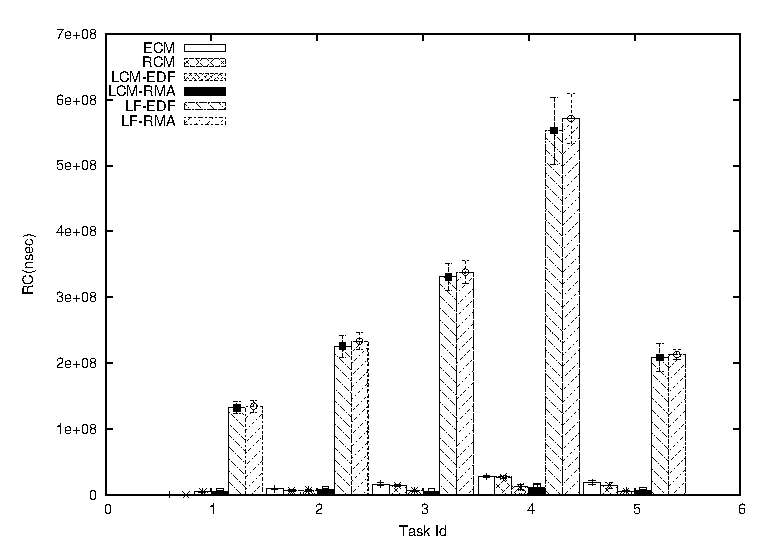
\includegraphics[scale=0.6]{figures/Abr_dur_5t_nl_g_30_0.2_0.2_0.2_1.eps}
\label{fig-RC-set1}
}
\subfigure[Task set 2]{
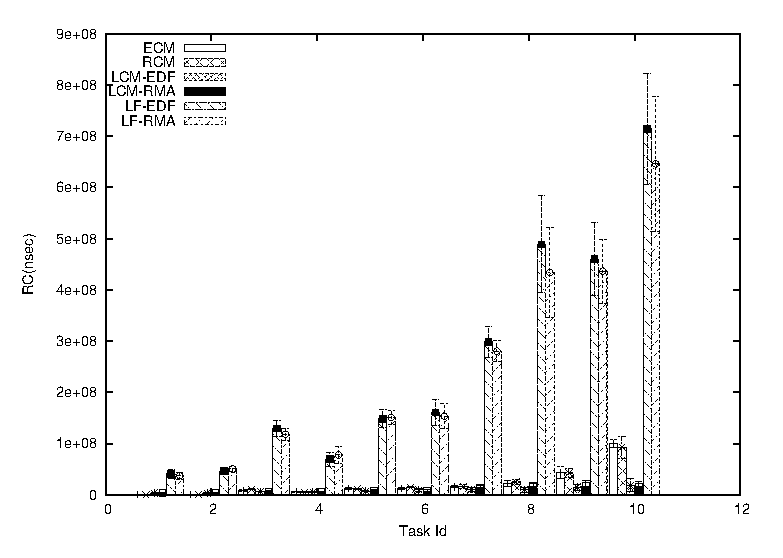
\includegraphics[scale=0.6]{figures/Abr_dur_10t_nl_g_30_0.2_0.2_0.2_1.eps}
\label{fig-RC-set2}
}
\subfigure[Task set 3]{
\includegraphics[scale=0.6]{figures/Abr_dur_12t_nl_g_30_0.2_0.2_0.2_1.eps}
\label{fig-RC-set3}
}
\caption{Task retry costs under LCM and competitor synchronization methods}
\label{fig:RC_results}
\end{figure}

Figure \ref{fig:res_results-1} shows the response time of each task of the task sets in Table \ref{pnf_task_sets_table} with a confidence level of 0.95. (Again, each task's atomic section length is equal to half of the task length.) 
We observe that G-EDF/LCM and G-RMA/LCM achieve shorter 
response time than the retry-loop lock-free
algorithm, and shorter 
or comparable response time than ECM and RCM.

\begin{figure}[htbp]
\subfigure[Task set 1]{
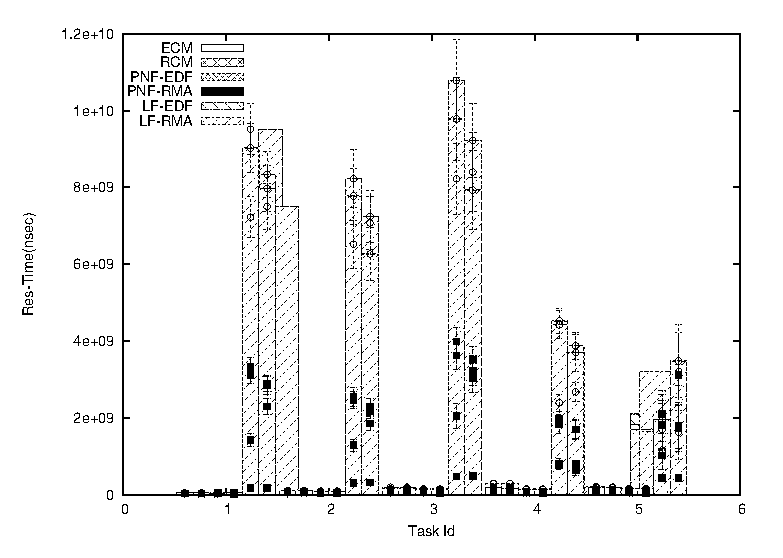
\includegraphics[scale=0.6]{figures/Res_Time_5t_nl_g_30_0.2_0.2_0.2_1.eps}
\label{fig-res-set1-1}
}
\subfigure[Task set 2]{
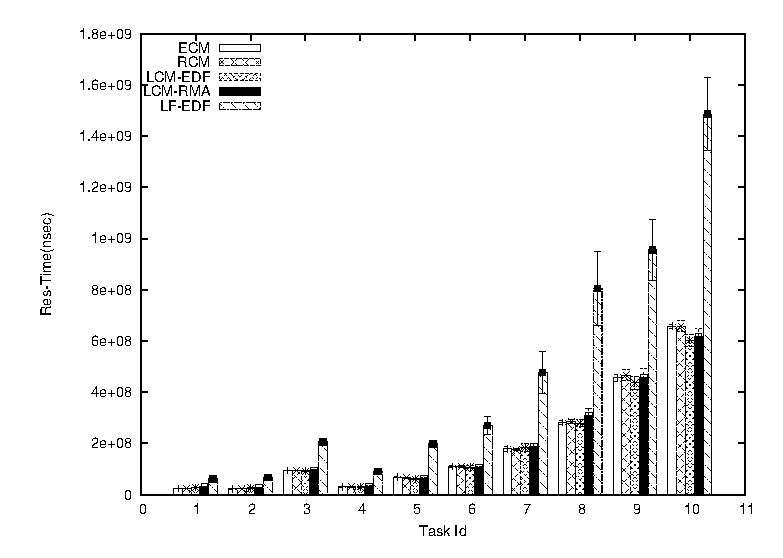
\includegraphics[scale=0.6]{figures/Res_Time_10t_nl_g_30_0.2_0.2_0.2_1.eps}
\label{fig-res-set2-1}
}
\subfigure[Task set 3 ]{
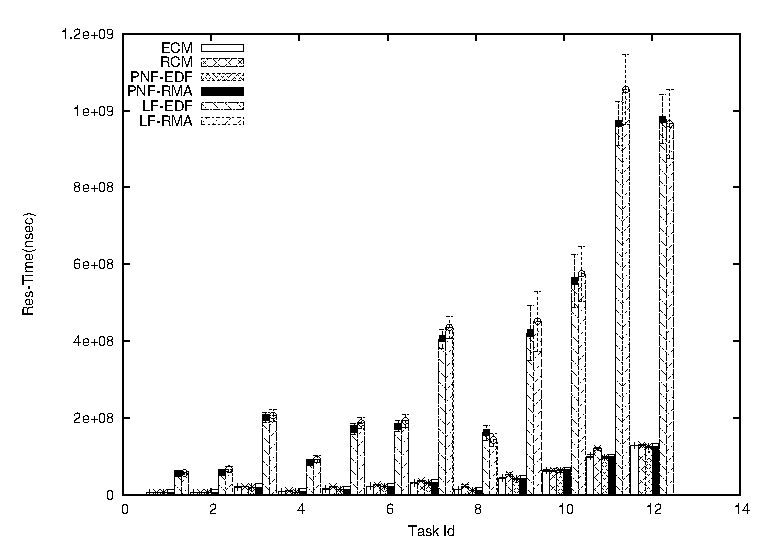
\includegraphics[scale=0.6]{figures/Res_Time_12t_nl_g_30_0.2_0.2_0.2_1.eps}
\label{fig-res-set3-1}
}
\caption{Task response times under LCM and competitor synchronization methods}
\label{fig:res_results-1}
\end{figure}

We repeated the experiments by varying the number and length of atomic sections. These results are shown in Appendix ~\ref{extended results}. Each figure's label has three parameters $x,y,z$. $x$ specifies the relative total length of all atomic sections to the length of the task. $y$ specifies the maximum relative length of any atomic section to the length of the task. $z$ specifies the minimum relative length of any atomic section to the length of the task. These figures show a consistent trend with previous results.

\subsection{PNF Results}
\label{pnf experiemtns}
 
The difficulty in testing with PNF is to incur transitive retry cases. Tasks are arranged in non-decreasing order of periods, and each task shares objects only with the previous and next tasks. Each task begins with an atomic section. Thus, increasing the opportunity of transitive retry.

Figure~\ref{fig:pnf_results_1_obj_all} shows average retry cost under ECM, RCM, LCM, PNF and lock-free for each task set. Figure~\ref{fig:pnf_results_1_obj_without_lock_free} shows average retry cost for only contention managers for each task set. The $x$-axis has three parameters $a,b,c$. $a$ specifies the relative total length of all atomic sections to the length of the task. $b$ specifies the maximum relative length of any atomic section to the length of the task. $c$ specifies the minimum relative length of any atomic section to the length of the task. Each data point in the figure has a confidence level of 0.95.
Only one object per transaction is shared in Figures~\ref{fig:pnf_results_1_obj_all} and~\ref{fig:pnf_results_1_obj_without_lock_free}.

Lock-free is the longest technique as it provides no conflict resolution. PNF better or comparable retry cost than ECM, RCM and LCM. As we move from 4 to 8 to 20 task set, retry costs of different contention managers get closer to each other. This is explained by noting that each task set in Table~\ref{pnf_task_sets_table} is organized in non-decreasing order of periods, and $c_i/T_i$ for almost each $\tau_i$ is low. Besides, each task shares objects only with the previous and next tasks, and tasks are released at the same time to enforce transitive retry. While the first instances of all tasks have a high potential of conflict, the contention level decreases with time for higher number of tasks. Thus, for the 20 task set, contention level is the lowest. Hence, retry costs of all contention managers get closer as number of tasks increases.

We compared retry cost for different contention managers with multiple objects per transaction and different levels of read/writer operations. Figure~\ref{fig:cm_20obj_per_tx_40wr} shows retry cost of the three task sets sharing 20 objects per transaction, with 40\% write operations and 60\% read operations. The same experiment is repeated in Figure~\ref{fig:cm_20obj_per_tx_80wr} with 80\% write operations, and 20\% read operations. Figure~\ref{fig:cm_20obj_per_tx_100wr} repeats the same experiment with 100\% write operations. The same previous three experiments were repeated in Figures~\ref{fig:cm_40obj_per_tx_40wr},~\ref{fig:cm_40obj_per_tx_80wr} and~\ref{fig:cm_40obj_per_tx_100wr} with 40 objects per transaction. Figures~\ref{fig:cm_20obj_per_tx_40wr} to~\ref{fig:cm_40obj_per_tx_100wr} show consistent trends with Figure~\ref{fig:pnf_results_1_obj_without_lock_free} except that retry cost of PNF is shorter than the others even with increasing number of tasks. For the 20 task set, PNF retry cost is a little shorter than LCM, but much better than ECM and RCM. This happens because of sharing multiple objects per transaction. Thus, contention level is increased than in sharing 1 object per transaction. Besides, transitive retry exists which makes PNF better than the others.
%%%%%%%%%%%%%%%%%%%%%%%%%%%%%%%%%%%%%%%%%%%%%%%%%%%%%%%

\begin{figure}[!htpd]
\centering

\subfigure[4 tasks]{
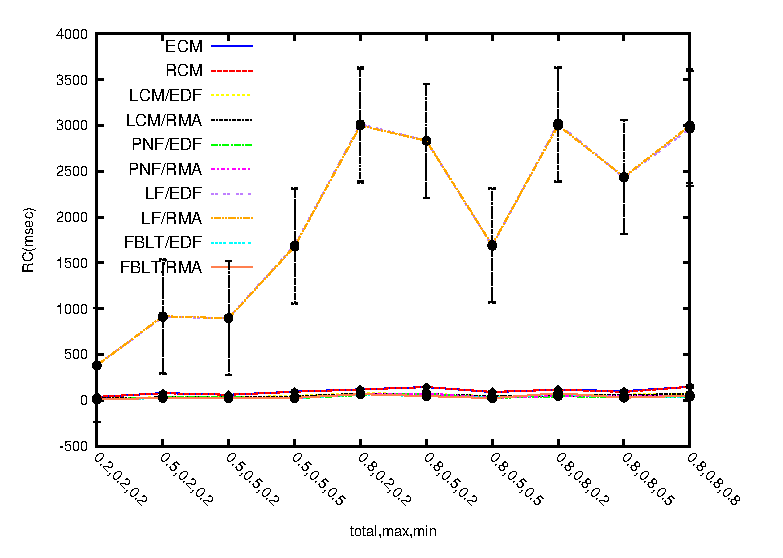
\includegraphics[scale=0.7]
{figures/Abr_dur_4t_5obj_all_100wr}
\label{fig:results_1_obj_all_4_tasks}
}
~
\subfigure[8 tasks]{
\includegraphics[scale=0.7]
{figures/Abr_dur_8t_9obj_all_100wr}
\label{fig:results_1_obj_all_8_tasks}
}
~
\subfigure[20 tasks]{
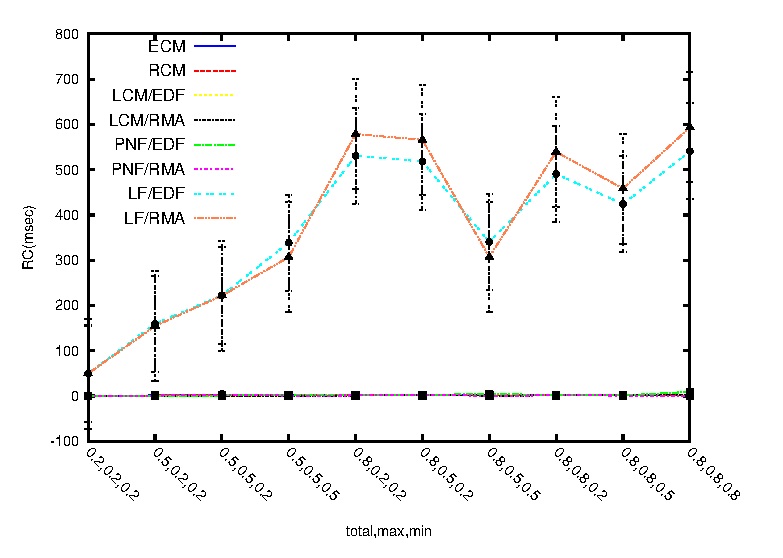
\includegraphics[scale=0.7]
{figures/Abr_dur_20t_21obj_all_100wr}
\label{fig:results_1_obj_all_20_tasks}
}
\caption{Average retry cost for 1 object per transaction for different values of total, maximum and minimum atomic section length under all synchronization techniques}
\label{fig:pnf_results_1_obj_all}
\end{figure}

\begin{figure}[!htpd]
\centering

\subfigure[4 tasks]{
\includegraphics[scale=0.7]
{figures/Abr_dur_4t_5obj_100wr}
\label{fig:pnf_results_1_obj_cm_4t}
}
~
\subfigure[8 tasks]{
\includegraphics[scale=0.7]
{figures/Abr_dur_8t_9obj_100wr}
\label{fig:pnf_results_1_obj_cm_8t}
}
~
\subfigure[20 tasks]{
\includegraphics[scale=0.7]
{figures/Abr_dur_20t_21obj_100wr}
\label{fig:pnf_results_1_obj_cm_20t}
}
\caption{Average retry cost for 1 object per transaction for different values of total, maximum and minimum atomic section length under contention managers only}
\label{fig:pnf_results_1_obj_without_lock_free}
\end{figure}
%%%%%%%%%%%%%%%%%%%%%%%%%%%%%%%%
\begin{figure}[!htpd]
\centering

\subfigure[4 tasks]{
\includegraphics[scale=0.7]
{figures/Abr_dur_4t_50obj_40wr}
\label{fig:4t_ecm_rcm_lcm_pnf_50obj_40wr}
}
~
\subfigure[8 tasks]{
\includegraphics[scale=0.7]
{figures/Abr_dur_8t_90obj_40wr}
\label{fig:8t_ecm_rcm_lcm_pnf_90obj_40wr}
}
~
\subfigure[20 tasks]{
\includegraphics[scale=0.7]
{figures/Abr_dur_20t_210obj_40wr}
\label{fig:20t_ecm_rcm_lcm_pnf_210obj_40wr}
}
\caption{Average retry cost for 20 objects per transaction, 40\% write operations for different values of total, maximum and minimum atomic section length under different CMs}
\label{fig:cm_20obj_per_tx_40wr}
\end{figure}
%%%%%%%%%%%%%%%%%%%%%%%%%%%%%%%%%%%%%%%%%%%%%%%%%%%%%%
%%%%%%%%%%%%%%%%%%%%%%%%%%%%%%%%
\begin{figure}[!htpd]
\centering

\subfigure[4 tasks]{
\includegraphics[scale=0.7]
{figures/Abr_dur_4t_50obj_80wr}
\label{fig:4t_ecm_rcm_lcm_pnf_50obj_80wr}
}
~
\subfigure[8 tasks]{
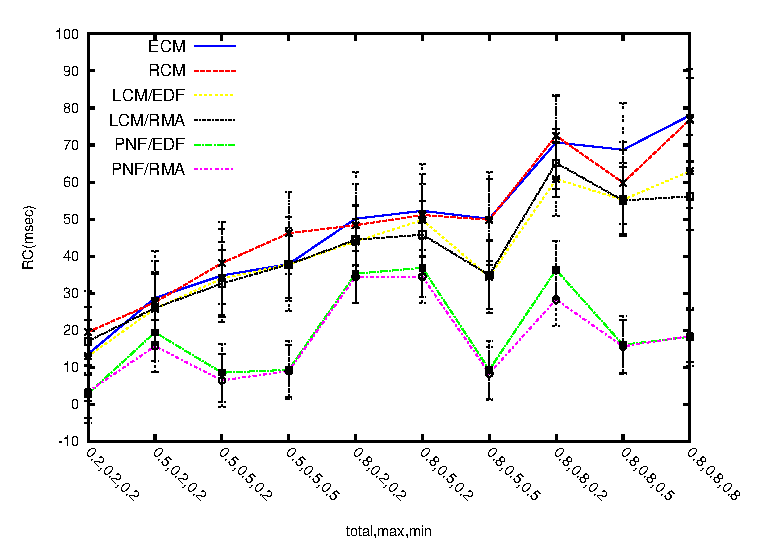
\includegraphics[scale=0.7]
{figures/Abr_dur_8t_90obj_80wr}
\label{fig:8t_ecm_rcm_lcm_pnf_90obj_80wr}
}
~
\subfigure[20 tasks]{
\includegraphics[scale=0.7]
{figures/Abr_dur_20t_210obj_80wr}
\label{fig:20t_ecm_rcm_lcm_pnf_210obj_80wr}
}
\caption{Average retry cost for 20 objects per transaction, 80\% write operations for different values of total, maximum and minimum atomic section length under different CMs}
\label{fig:cm_20obj_per_tx_80wr}
\end{figure}
%%%%%%%%%%%%%%%%%%%%%%%%%%%%%%%%%%%%%%%%%%%%%%%%%%%%%%
\begin{figure}[!htpd]
\centering

\subfigure[4 tasks]{
\includegraphics[scale=0.7]
{figures/Abr_dur_4t_50obj_100wr}
\label{fig:4t_ecm_rcm_lcm_pnf_50obj_100wr}
}
~
\subfigure[8 tasks]{
\includegraphics[scale=0.7]
{figures/Abr_dur_8t_90obj_100wr}
\label{fig:8t_ecm_rcm_lcm_pnf_90obj_100wr}
}
~
\subfigure[20 tasks]{
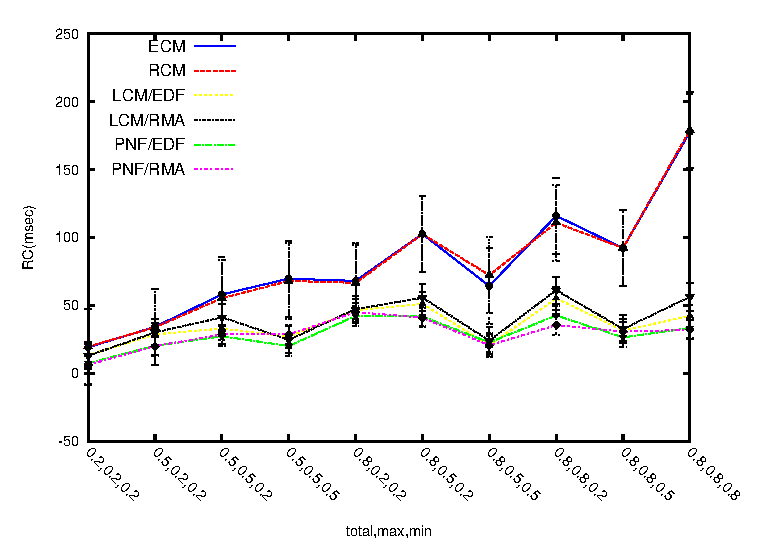
\includegraphics[scale=0.7]
{figures/Abr_dur_20t_210obj_100wr}
\label{fig:20t_ecm_rcm_lcm_pnf_210obj_100wr}
}
\caption{Average retry cost for 20 objects per transaction, 100\% write operations for different values of total, maximum and minimum atomic section length under different CMs}
\label{fig:cm_20obj_per_tx_100wr}
\end{figure}
%%%%%%%%%%%%%%%%%%%%%%%%%%%%%%%%%%%%%%%%%%%%%%%%%%%%%%
\begin{figure}[!htpd]
\centering

\subfigure[4 tasks]{
\includegraphics[scale=0.7]
{figures/Abr_dur_4t_100obj_40wr}
\label{fig:4t_ecm_rcm_lcm_pnf_100obj_40wr}
}
~
\subfigure[8 tasks]{
\includegraphics[scale=0.7]
{figures/Abr_dur_8t_180obj_40wr}
\label{fig:8t_ecm_rcm_lcm_pnf_180obj_40wr}
}
~
\subfigure[20 tasks]{
\includegraphics[scale=0.7]
{figures/Abr_dur_20t_420obj_40wr}
\label{fig:20t_ecm_rcm_lcm_pnf_420obj_40wr}
}
\caption{Average retry cost for 40 objects per transaction, 40\% write operations for different values of total, maximum and minimum atomic section length under different CMs}
\label{fig:cm_40obj_per_tx_40wr}
\end{figure}
%%%%%%%%%%%%%%%%%%%%%%%%%%%%%%%%%%%%%%%%%%%%%%%%%%%%%%
\begin{figure}[!htpd]
\centering

\subfigure[4 tasks]{
\includegraphics[scale=0.7]
{figures/Abr_dur_4t_100obj_80wr}
\label{fig:4t_ecm_rcm_lcm_pnf_100obj_80wr}
}
~
\subfigure[8 tasks]{
\includegraphics[scale=0.7]
{figures/Abr_dur_8t_180obj_80wr}
\label{fig:8t_ecm_rcm_lcm_pnf_180obj_80wr}
}
~
\subfigure[20 tasks]{
\includegraphics[scale=0.7]
{figures/Abr_dur_20t_420obj_80wr}
\label{fig:20t_ecm_rcm_lcm_pnf_420obj_80wr}
}
\caption{Average retry cost for 40 objects per transaction, 80\% write operations for different values of total, maximum and minimum atomic section length under different CMs}
\label{fig:cm_40obj_per_tx_80wr}
\end{figure}
%%%%%%%%%%%%%%%%%%%%%%%%%%%%%%%%%%%%%%%%%%%%%%%%%%%%%%
\begin{figure}[!htpd]
\centering

\subfigure[4 tasks]{
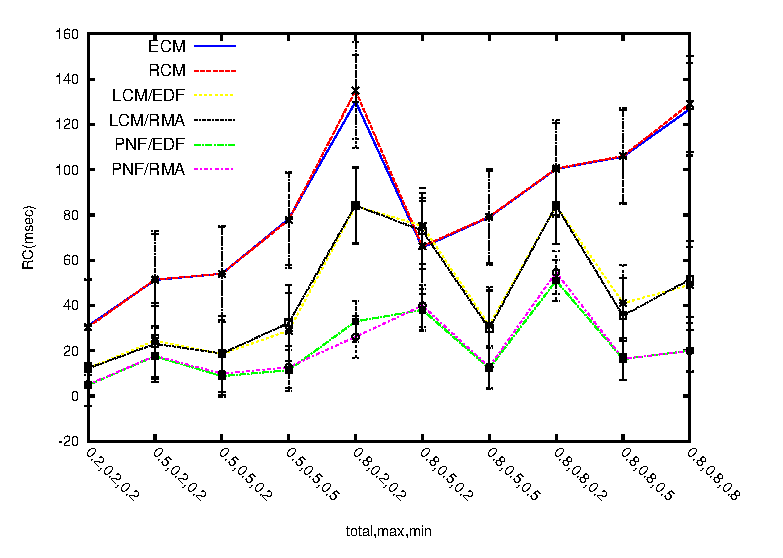
\includegraphics[scale=0.7]
{figures/Abr_dur_4t_100obj_100wr}
\label{fig:4t_ecm_rcm_lcm_pnf_100obj_100wr}
}
~
\subfigure[8 tasks]{
\includegraphics[scale=0.7]
{figures/Abr_dur_8t_180obj_100wr}
\label{fig:8t_ecm_rcm_lcm_pnf_180obj_100wr}
}
~
\subfigure[20 tasks]{
\includegraphics[scale=0.7]
{figures/Abr_dur_20t_420obj_100wr}
\label{fig:20t_ecm_rcm_lcm_pnf_420obj_100wr}
}
\caption{Average retry cost for 40 objects per transaction, 100\% write operations for different values of total, maximum and minimum atomic section length under different CMs}
\label{fig:cm_40obj_per_tx_100wr}
\end{figure}

\subsection{FBLT Results}
\label{fblt experiemnt sec}

We repeated the experiments in Section~\ref{pnf experiemtns} including FBLT. While Figure~\ref{fig:fblt_results_1_obj_all} includes all synchronization methods, Figure~\ref{fig:fblt_results_1_obj_without_lock_free} excludes lock-free. From these figures, we observe that lock-free has the largest retry cost, as it provides no conflict resolution. FBLT has the largest retry cost among CMs,  because transactions share only one object in this case. For multiple objects per transaction, FBLT provides equal or shorter retry cost than LCM, as shown in Figures~\ref{fig-RC-fblt-4t-20obj} and~\ref{fig-RC-fblt-4t-40obj}. PNF has an advantage over FBLT. However, PNF requires a-priori knowledge of all objects accessed by each transaction, whereas FBLT does not. Consequently, retry cost under PNF is shorter than that under FBLT. For 8 and 20 task sets, FBLT's retry cost is comparable to PNF's as shown in Figures~\ref{fig-RC-fblt-8t-20obj} to~\ref{fig-RC-fblt-20t-40obj}. So, experiments show that FBLT's retry cost can be shorter than that under ECM, RCM, and LCM, and can be comparable to that of PNF's.

\begin{figure}[!htpd]
\centering
\subfigure[ECM, RCM, LCM, PNF, FBLT, Lock-Free]{
\includegraphics[scale=0.6]
{/e/lectures/real-time/PhD-work/STM/Practical/results_uno/figures/5_tasks/Abr_Dur/fblt/Abr_dur_5t_1obj_all_100wr}
\label{fig:fblt_results_1_obj_all}
}
%~
\subfigure[ECM, RCM, LCM, PNF, FBLT]{
\includegraphics[scale=0.6]
{/e/lectures/real-time/PhD-work/STM/Practical/results_uno/figures/5_tasks/Abr_Dur/fblt/Abr_dur_5t_1obj_100wr}
\label{fig:fblt_results_1_obj_without_lock_free}
}
\caption{Avgerage retry cost (one object/transaction).}

\label{fig:fblt_results_uniobject}
\end{figure}\begin{figure}
\centering
\subfigure[ECM, RCM, LCM, PNF, FBLT, Lock-Free]{
\includegraphics[scale=0.6]
{/e/lectures/real-time/PhD-work/STM/Practical/results_uno/figures/5_tasks/Abr_Dur/fblt/Abr_dur_5t_1obj_all_100wr}
\label{fig:fblt_results_1_obj_all}
}
%~
\subfigure[ECM, RCM, LCM, PNF, FBLT]{
\includegraphics[scale=0.6]
{/e/lectures/real-time/PhD-work/STM/Practical/results_uno/figures/5_tasks/Abr_Dur/fblt/Abr_dur_5t_1obj_100wr}
\label{fig:fblt_results_1_obj_without_lock_free}
}
\caption{Avgerage retry cost (one object/transaction).}

\label{fig:fblt_results_uniobject}
\end{figure}


\begin{figure}[!htpd]
\centering
\includegraphics[scale=0.6]{/e/lectures/real-time/PhD-work/STM/Practical/results_uno/figures/4_tasks/Abr_Dur/fblt/Abr_dur_4t_50obj_100wr_-1eta}
\caption{Avgerage retry cost (20 shared objects, 4 tasks).}
\label{fig-RC-fblt-4t-20obj}
\end{figure}

\begin{figure}[!htpd]
\centering
\includegraphics[scale=0.6]{/e/lectures/real-time/PhD-work/STM/Practical/results_uno/figures/4_tasks/Abr_Dur/fblt/Abr_dur_4t_100obj_100wr_-1eta}
\caption{Avgerage retry cost (40 shared objects, 4 tasks).}
\label{fig-RC-fblt-4t-40obj}
\end{figure}

\begin{figure}[!htpd]
\centering
\includegraphics[scale=0.6]{/e/lectures/real-time/PhD-work/STM/Practical/results_uno/figures/8_tasks/Abr_Dur/fblt/Abr_dur_8t_90obj_100wr_-1eta}
\caption{Avgerage retry cost (20 shared objects, 8 tasks).}
\label{fig-RC-fblt-8t-20obj}
\end{figure}

\begin{figure}[!htpd]
\centering
\includegraphics[scale=0.6]{/e/lectures/real-time/PhD-work/STM/Practical/results_uno/figures/8_tasks/Abr_Dur/fblt/Abr_dur_8t_180obj_100wr_-1eta}
\caption{Avgerage retry cost (40 shared objects, 8 tasks).}
\label{fig-RC-fblt-8t-40obj}
\end{figure}

\begin{figure}[!htpd]
\centering
\includegraphics[scale=0.6]{/e/lectures/real-time/PhD-work/STM/Practical/results_uno/figures/20_tasks/Abr_Dur/fblt/Abr_dur_20t_210obj_100wr_-1eta}
\caption{Avgerage retry cost (20 shared objects, 20 tasks).}
\label{fig-RC-fblt-20t-20obj}
\end{figure}

\begin{figure}[!htpd]
\centering
\includegraphics[scale=0.6]{/e/lectures/real-time/PhD-work/STM/Practical/results_uno/figures/20_tasks/Abr_Dur/fblt/Abr_dur_20t_420obj_100wr_-1eta}
\caption{Avgerage retry cost (40 shared objects, 20 tasks).}
\label{fig-RC-fblt-20t-40obj}
\end{figure}

PNF was designed to avoid transitive retry. Previous experiments compares retry cost of different CMs in case of transitive retry. Figures~\ref{fig-RC-fblt-4t-20obj} to~\ref{fig-RC-fblt-20t-20obj}  compare retry costs of different CMs in case of non-transitive retry. FBLT achieves shorter or comparable retry cost to other CMs including PNF.

\begin{figure}[!htpd]
\centering
\includegraphics[scale=0.6]{/e/lectures/real-time/PhD-work/STM/Practical/results_uno/figures/4_tasks/Abr_Dur/fblt/Abr_dur_4t_20obj_100wr_-1eta}
\caption{Avgerage retry cost (20 shared objects, 4 tasks).}
\label{fig-RC-fblt-20t-20obj}
\end{figure}

\begin{figure}[!htpd]
\centering
\includegraphics[scale=0.6]{/e/lectures/real-time/PhD-work/STM/Practical/results_uno/figures/8_tasks/Abr_Dur/fblt/Abr_dur_8t_20obj_100wr_-1eta}
\caption{Avgerage retry cost (20 shared objects, 8 tasks).}
\label{fig-RC-fblt-8t-20obj}
\end{figure}

%\begin{comment}
\begin{figure}[!htpd]
\centering
\includegraphics[scale=0.6]{/e/lectures/real-time/PhD-work/STM/Practical/results_uno/figures/20_tasks/Abr_Dur/fblt/Abr_dur_20t_20obj_100wr_-1eta}
\caption{Avgerage retry cost (20 shared objects, 20 tasks).}
\label{fig-RC-fblt-20t-20obj}
\end{figure}
%\end{comment}

%\newpage


\section{Conclusions}
\label{sec:conclusions}

We designed, analyzed, and experimentally evaluated four real-time CMs. Designing real-time CMs is straightforward. The simplest logic is to use the same rationale as that of the underlying real-time scheduler. This was shown in the design of ECM and RCM. ECM allows the transaction with the earliest absolute deadline (i.e., dynamic priority) to commit first. RCM allows the transaction with the smallest period (i.e., fixed priority) to commit first. We established upper bounds for retry costs and response times under ECM and RCM, and identified the conditions under which they have better schedulability than lock-free synchronization. 

Under both ECM and RCM, a task incurs $2.s_{max}$ retry cost for each of its atomic sections due to a conflict with another task's atomic section. Retries under RCM and lock-free synchronization are affected by a larger number of conflicting task instances than under ECM. While task retries under ECM and lock-free are affected by all other tasks, retries under RCM are affected only by higher priority tasks. 

STM and lock-free synchronization have similar parameters that affect their retry costs -- i.e., the number of conflicting jobs and how many times they access shared objects. The $s_{max}/r_{max}$ ratio determines whether STM is better or as good as lock-free. For ECM, this ratio cannot exceed 1, and it can be 1/2 for higher number of conflicting tasks. For RCM, for the common case, $s_{max}$ must be 1/2 of $r_{max}$, and in some cases, $s_{max}$ can be larger than $r_{max}$ by many orders of magnitude.

LCM, which can be used with both G-EDF and G-RMA, tries to compromise between priority of transactions (which is the priority of the underlying tasks), and the remaining execution time of the interfered transaction. As the remaining execution time of the interfered transaction decreases, it is not effective to abort the transaction when it can shortly commit. The parameters $\alpha$ and $\psi$ are used to determine whether or not to abort the interfered transaction. $\alpha$ ranges between 0 and 1. When $\alpha \rightarrow 0$, LCM defaults to FCFS. When $\alpha\rightarrow1$, G-EDF/LCM defaults to ECM, and G-RMA/LCM defaults to RCM. We also derived upper bounds on retry costs and response times under LCM, and compared the schedulability of LCM with ECM, RCM, and lock-free synchronization. Also, we identified the conditions under which LCM performs better than the other synchronization techniques. LCM reduces the retry cost  of each atomic section to $(1+\alpha_{max})s_{max}$, instead of $2.s_{max}$ as in ECM and RCM. In ECM and RCM, tasks do not retry due to lower priority tasks, whereas in LCM, they do so. In G-EDF/LCM, retry due to a lower priority job is encountered only from a task $\tau_{j}$'s last job instance during $\tau_{i}$'s period. This is not the case with G-RMA/LCM, because,  each higher priority task can be aborted and retried by any job instance of lower priority tasks. 

Schedulability of G-EDF/LCM and G-RMA/LCM is better or equal to ECM and RCM, respectively, by proper choices for $\alpha_{min}$ and $\alpha_{max}$. Schedulability of G-EDF/LCM and G-RMA/LCM is better or equal to lock-free synchronization as long as $s_{max}/r_{max}$ does not exceed 0.5. By proper choice of $\alpha$s, $s_{max}/r_{max}$ can be increased to 2 under G-EDF/LCM, and to larger values under G-RMA/LCM.

ECM, RCM, and LCM are affected by transitive retry. Transitive retry occurs when a transaction accesses multiple objects. It causes a transaction to abort and retry  due to another non-conflicting transaction. PNF avoids transitive retry, and and also optimizes the processor usage by reducing the priority of the aborted transaction. This way, other tasks can proceed if they do not conflict with other executing transactions. 

We upper bounded PNF's retry cost and response time. We also compared PNF's schedulability to other synchronization techniques. PNF has better schedulability than lock-free synchronization as long as $s_{max}$ does not exceed $r_{max}$. 

We also implemented the CMs and conducted experimental studies. Our experimental studies revealed that the CMs' have shorter retry costs than lock-free synchronization. In particular, PNF has shorter retry costs than others as long as transitive retry and contention exist. However, PNF's implementation is relatively complex. 

PNF requires a-priori knowledge about objects accessed by each transaction. This is incompatible with dynamic STM implementations. Thus, we introduce the FBLT contention manager. Under  FBLT, each transaction is allowed to abort for a no larger than a specified number of times. Afterwards, the transaction becomes non-preemptive. Non-preemptive transactions have higher priorities than other preemptive transactions and real-time jobs. Non-preemptive transactions resolve their conflicts using FIFO order.

By proper adjustment of the maximum abort number of each transaction, we showed that FBLT's schedulability is equal to or better than other synchronization techniques. For FBLT's schedulability to be equal to or better than lock-free synchronization, the upper bound on $s_{max}/r_{max}$ must be 1. The upper bound on $s_{max}/r_{max}$ can be higher than 1 if transactions execute in their arrival order and contention is high.

Our experimental results show that FBLT has equal or shorter retry cost than ECM, RCM, and LCM. PNF requires a-priori knowledge of all objects accessed by each transaction. This is an advantage for PNF over FBLT. Consequently, retry cost under PNF is shorter than that under FBLT. Still, FBLT's retry cost can be comparable to PNF's.

Our experimental results show that FBLT has equal or shorter retry cost than ECM, RCM, and LCM. PNF requires a-priori knowledge of all objects accessed by each transaction. This is an advantage for PNF over FBLT. Consequently, retry cost under PNF is shorter than that under FBLT in case of transitive retry. Still, FBLT's retry cost can be comparable to PNF's. In case of no or low transitive retry, FBLT achieves shorter retry cost than other CMs including PNF.

Future work includes choosing another criterion to resolve conflicts of non-preemptive transactions. Also, using feedback from the system to adjust maximum abort number of each transaction. Consequently, retry cost can be reduced over time.




\bibliographystyle{plain}
\bibliography{/e/lectures/real-time/PhD-work/STM/writing/global_bibliography/global_bibliography.bib}

\pagebreak 
%\newpage{}
\appendix
\section{\label{notations}Notations}

%\section{Notation}

%\begin{table*}
%\caption{\label{table 3}Used notations}
\begin{adjustwidth}{-1.5cm}{}
\begin{flushleft}
\begin{tabular}{|>{\raggedright}p{2.5cm}|>{\raggedright}p{12cm}|}
\hline 
$T_{i}$ & \raggedright{}Task $i$.\tabularnewline
\hline 
$T_{i}^{j}$ & $j^{th}$ Instance (job) of task $i$.\tabularnewline
\hline 
$t(T_{i})$ & Minumum period of $T_{i}$.\tabularnewline
\hline 
$D(T_{i})$ & Relative deadline of any instance of $T_{i}$\tabularnewline
\hline 
$r(T_{i}^{j})$ & Release time of job $T_{i}^{j}$.\tabularnewline
\hline 
$d(T_{i}^{j})$ & Absolute deadline of $T_{i}^{j}$.\tabularnewline
\hline 
$c_{j}$ & WCET of any instance of $T_{j}$\tabularnewline
\hline 
$p(T_{i})$ & \raggedright{}Priority of $T_{i}$.\tabularnewline
\hline 
$c_{ji}$ & The new WCET of $T_{j}$ relative to the studied task $T_{i}$. This
length changes according to the studied task.\tabularnewline
\hline 
$\theta$ & An object that can be accessed by any task.\tabularnewline
\hline 
$\theta_{i}$ & Set of objects accessed by $T_{i}$ without repeatition.\tabularnewline
\hline 
$\gamma(\theta)$ & Set of tasks that share object $\theta$ with $T_{i}$.\tabularnewline
\hline 
$s_{i}(\theta)$ & Set of atomic sections of $T_{i}$ that access object $\theta$.\tabularnewline
\hline 
$s(\theta)$ & Set of atomic sections in all tasks that share object $\theta$.\tabularnewline
\hline 
$s_{i}^{k}(\theta)$ & The $k^{th}$ atomic section of $T_{i}$ that accesses object $\theta$.\tabularnewline
\hline 
$s_{i}^{k}$ & The $k^{th}$ atomic section of $T_{i}$ regrdless of which object
it accesses.\tabularnewline
\hline 
$s_{i}$ & Set of atomic sections in $T_{i}$.\tabularnewline
\hline 
$len(s_{i}^{k}(\theta))$ & Length of $s_{i}^{k}(\theta)$.\tabularnewline
\hline 
$len(s_{i}(\theta))$ & Sum of all atomic sections in $T_{i}$ that access object $\theta$.\tabularnewline
\hline 
$s_{max}(\theta)$ & The maximum atomic section in all tasks that share object $\theta$.\tabularnewline
\hline 
$s_{i_{max}}(\theta)$ & The maximum atomic section in $T_{i}$ that accesses object $\theta$.\tabularnewline
\hline 
$s_{max}^{i}(\theta)$ & The maximum atomic section in all tasks with priority lower than or
equal to that of $T_{i}$ that share object $\theta$.\tabularnewline
\hline 
$W_{i}^{p}(s_{j}^{k}(\theta))$ & Contribution or workload by $s_{j}^{k}(\theta)$ in the retrial cost
of $s_{i}^{p}(\theta)$.\tabularnewline
\hline 
$RC(T_{i})$ & Maximum transactional retrial cost of atomic sections in $T_{i}$
due to conflict between atomic sections.\tabularnewline
\hline 
$RC(L(T_{i}))$ & The same as $RC(T_{i})$ but calculated only in a period of length
$L$.\tabularnewline
\hline 
$RC(t(T_{i}))$ & The same as $RC(T_{i})$ over the whole $t(T_{i})$.\tabularnewline
\hline 
$G_{ij}(L)$ & Number of interferences made by $T_{j}$ to $T_{i}$ during period
of length $L$.\tabularnewline
\hline 
$W_{ij}(L)$ & \raggedright{}Workload contributed by $T_{j}$ to $T_{i}$ during
period of length $L$.\tabularnewline
\hline 
$s\_\theta$ & A short resource.\tabularnewline
\hline 
$l\_\theta$ & A long resource.\tabularnewline
\hline 
$g(s\_\theta)$ & A group containing only short resource.\tabularnewline
\hline 
$g(l\_\theta)$ & A group containing only long resources.\tabularnewline
\hline 
$R_{k}(g(s\_\theta))$ & Request made by $T_{k}$ to the $g(s\_\theta)$.\tabularnewline
\hline 
$R_{k}(g(l\_\theta))$ & Request made by $T_{k}$ to the $g(l\_\theta)$.\tabularnewline
\hline 
$|R_{k}(g(s\_\theta))|$ & The size of the request and it equals the sum of all nested accesses
to resources in $g(s\_\theta)$ made by $T_{k}$.\tabularnewline
\hline 
$|R_{k}(g(l\_\theta))|$ & The sum of nested requests by $T_{k}$ to the group containing $l\_\theta$,
plus $max_{s\_\theta\in\theta_{k}}[\sum_{h=1,h\ne k}^{min(m,n)-1}|R_{h}(g(s\_\theta))|]$,
if $s\_\theta$ can be called inside $l\_\theta$.\tabularnewline
\hline 
$N_{i,l}$ & The number of times $T_{i}^{j}$ requests long resources.\tabularnewline
\hline 
$N_{i,s}$ & The number of times $T_{i}^{j}$ requests short resources.\tabularnewline
\hline
\end{tabular}
\par\end{flushleft}
\end{adjustwidth}
%\end{table*}

\section{\label{extended results}Extended Results}

\begin{figure}[!htpd]
\centering
\subfigure[Task set 1]{
\includegraphics[scale=0.6]
{figures/Abr_dur_5t_nl_g_30_0.5_0.2_0.2_1.eps}
\label{Abr_dur_5t_nl_g_30_0.5_0.2_0.2_1.eps}
}
\subfigure[Task set 2]{
\includegraphics[scale=0.6]
{figures/Abr_dur_10t_nl_g_30_0.5_0.2_0.2_1.eps}
\label{Abr_dur_10t_nl_g_30_0.5_0.2_0.2_1.eps}
}
\subfigure[Task set 3]{
\includegraphics[scale=0.6]
{figures/Abr_dur_12t_nl_g_30_0.5_0.2_0.2_1.eps}
\label{Abr_dur_12t_nl_g_30_0.5_0.2_0.2_1.eps}
}
\caption{Task retry costs under LCM and competitor synchronization methods (0.5,0.2,0.2)}
\label{fig:RC_results 0.5 0.2 0.2}
\end{figure}
%

\begin{figure}[!htpd]
\centering
\subfigure[Task set 1]{
\includegraphics[scale=0.6]
{figures/Res_Time_5t_nl_g_30_0.5_0.2_0.2_1.eps}
\label{Res_Time_5t_nl_g_30_0.5_0.2_0.2_1.eps}
}
\subfigure[Task set 2]{
\includegraphics[scale=0.6]
{figures/Res_Time_10t_nl_g_30_0.5_0.2_0.2_1.eps}
\label{Res_Time_10t_nl_g_30_0.5_0.2_0.2_1.eps}
}
\subfigure[Task set 3]{
\includegraphics[scale=0.6]
{figures/Res_Time_12t_nl_g_30_0.5_0.2_0.2_1.eps}
\label{Res_Time_12t_nl_g_30_0.5_0.2_0.2_1.eps}
}
\caption{Task response times under LCM and competitor synchronization methods (0.5,0.2,0.2)}
\label{fig:res_results 0.5 0.2 0.2}
\end{figure}
%

\begin{figure}[!htpd]
\centering
\subfigure[Task set 1]{
\includegraphics[scale=0.6]
{figures/Abr_dur_5t_nl_g_30_0.5_0.5_0.2_1.eps}
\label{Abr_dur_5t_nl_g_30_0.5_0.5_0.2_1.eps}
}
\subfigure[Task set 2]{
\includegraphics[scale=0.6]
{figures/Abr_dur_10t_nl_g_30_0.5_0.5_0.2_1.eps}
\label{Abr_dur_10t_nl_g_30_0.5_0.5_0.2_1.eps}
}
\subfigure[Task set 3]{
\includegraphics[scale=0.6]
{figures/Abr_dur_12t_nl_g_30_0.5_0.5_0.2_1.eps}
\label{Abr_dur_12t_nl_g_30_0.5_0.5_0.2_1.eps}
}
\caption{Task retry costs under LCM and competitor synchronization methods (0.5,0.5,0.2)}
\label{fig:RC_results 0.5 0.5 0.2}
\end{figure}
%

\begin{figure}[!htpd]
\centering
\subfigure[Task set 1]{
\includegraphics[scale=0.6]
{figures/Res_Time_5t_nl_g_30_0.5_0.5_0.2_1.eps}
\label{Res_Time_5t_nl_g_30_0.5_0.5_0.2_1.eps}
}
\subfigure[Task set 2]{
\includegraphics[scale=0.6]
{figures/Res_Time_10t_nl_g_30_0.5_0.5_0.2_1.eps}
\label{Res_Time_10t_nl_g_30_0.5_0.5_0.2_1.eps}
}
\subfigure[Task set 3]{
\includegraphics[scale=0.6]
{figures/Res_Time_12t_nl_g_30_0.5_0.5_0.2_1.eps}
\label{Res_Time_12t_nl_g_30_0.5_0.5_0.2_1.eps}
}
\caption{Task response times under LCM and competitor synchronization methods (0.5,0.5,0.2)}
\label{fig:res_results 0.5 0.5 0.2}
\end{figure}
%

\begin{figure}[!htpd]
\centering
\subfigure[Task set 1]{
\includegraphics[scale=0.6]
{figures/Abr_dur_5t_nl_g_30_0.5_0.5_0.5_1.eps}
\label{Abr_dur_5t_nl_g_30_0.5_0.5_0.5_1.eps}
}
\subfigure[Task set 2]{
\includegraphics[scale=0.6]
{figures/Abr_dur_10t_nl_g_30_0.5_0.5_0.5_1.eps}
\label{Abr_dur_10t_nl_g_30_0.5_0.5_0.5_1.eps}
}
\subfigure[Task set 3]{
\includegraphics[scale=0.6]
{figures/Abr_dur_12t_nl_g_30_0.5_0.5_0.5_1.eps}
\label{Abr_dur_12t_nl_g_30_0.5_0.5_0.5_1.eps}
}
\caption{Task retry costs under LCM and competitor synchronization methods (0.5,0.5,0.5)}
\label{fig:RC_results 0.5 0.5 0.5}
\end{figure}
%

\begin{figure}[!htpd]
\centering
\subfigure[Task set 1]{
\includegraphics[scale=0.6]
{figures/Res_Time_5t_nl_g_30_0.5_0.5_0.5_1.eps}
\label{Res_Time_5t_nl_g_30_0.5_0.5_0.5_1.eps}
}
\subfigure[Task set 2]{
\includegraphics[scale=0.6]
{figures/Res_Time_10t_nl_g_30_0.5_0.5_0.5_1.eps}
\label{Res_Time_10t_nl_g_30_0.5_0.5_0.5_1.eps}
}
\subfigure[Task set 3]{
\includegraphics[scale=0.6]
{figures/Res_Time_12t_nl_g_30_0.5_0.5_0.5_1.eps}
\label{Res_Time_12t_nl_g_30_0.5_0.5_0.5_1.eps}
}
\caption{Task response times under LCM and competitor synchronization methods (0.5,0.5,0.5)}
\label{fig:res_results 0.5 0.5 0.5}
\end{figure}
%

\begin{figure}[!htpd]
\centering
\subfigure[Task set 1]{
\includegraphics[scale=0.6]
{figures/Abr_dur_5t_nl_g_30_0.8_0.2_0.2_1.eps}
\label{Abr_dur_5t_nl_g_30_0.8_0.2_0.2_1.eps}
}
\subfigure[Task set 2]{
\includegraphics[scale=0.6]
{figures/Abr_dur_10t_nl_g_30_0.8_0.2_0.2_1.eps}
\label{Abr_dur_10t_nl_g_30_0.8_0.2_0.2_1.eps}
}
\subfigure[Task set 3]{
\includegraphics[scale=0.6]
{figures/Abr_dur_12t_nl_g_30_0.8_0.2_0.2_1.eps}
\label{Abr_dur_12t_nl_g_30_0.8_0.2_0.2_1.eps}
}
\caption{Task retry costs under LCM and competitor synchronization methods (0.8,0.2,0.2)}
\label{fig:RC_results 0.8 0.2 0.2}
\end{figure}
%

\begin{figure}[!htpd]
\centering
\subfigure[Task set 1]{
\includegraphics[scale=0.6]
{figures/Res_Time_5t_nl_g_30_0.8_0.2_0.2_1.eps}
\label{Res_Time_5t_nl_g_30_0.8_0.2_0.2_1.eps}
}
\subfigure[Task set 2]{
\includegraphics[scale=0.6]
{figures/Res_Time_10t_nl_g_30_0.8_0.2_0.2_1.eps}
\label{Res_Time_10t_nl_g_30_0.8_0.2_0.2_1.eps}
}
\subfigure[Task set 3]{
\includegraphics[scale=0.6]
{figures/Res_Time_12t_nl_g_30_0.8_0.2_0.2_1.eps}
\label{Res_Time_12t_nl_g_30_0.8_0.2_0.2_1.eps}
}
\caption{Task response times under LCM and competitor synchronization methods (0.8,0.2,0.2)}
\label{fig:res_results 0.8 0.2 0.2}
\end{figure}
%

\begin{figure}[!htpd]
\centering
\subfigure[Task set 1]{
\includegraphics[scale=0.6]
{figures/Abr_dur_5t_nl_g_30_0.8_0.5_0.2_1.eps}
\label{Abr_dur_5t_nl_g_30_0.8_0.5_0.2_1.eps}
}
\subfigure[Task set 2]{
\includegraphics[scale=0.6]
{figures/Abr_dur_10t_nl_g_30_0.8_0.5_0.2_1.eps}
\label{Abr_dur_10t_nl_g_30_0.8_0.5_0.2_1.eps}
}
\subfigure[Task set 3]{
\includegraphics[scale=0.6]
{figures/Abr_dur_12t_nl_g_30_0.8_0.5_0.2_1.eps}
\label{Abr_dur_12t_nl_g_30_0.8_0.5_0.2_1.eps}
}
\caption{Task retry costs under LCM and competitor synchronization methods (0.8,0.5,0.2)}
\label{fig:RC_results 0.8 0.5 0.2}
\end{figure}
%

\begin{figure}[!htpd]
\centering
\subfigure[Task set 1]{
\includegraphics[scale=0.6]
{figures/Res_Time_5t_nl_g_30_0.8_0.5_0.2_1.eps}
\label{Res_Time_5t_nl_g_30_0.8_0.5_0.2_1.eps}
}
\subfigure[Task set 2]{
\includegraphics[scale=0.6]
{figures/Res_Time_10t_nl_g_30_0.8_0.5_0.2_1.eps}
\label{Res_Time_10t_nl_g_30_0.8_0.5_0.2_1.eps}
}
\subfigure[Task set 3]{
\includegraphics[scale=0.6]
{figures/Res_Time_12t_nl_g_30_0.8_0.5_0.2_1.eps}
\label{Res_Time_12t_nl_g_30_0.8_0.5_0.2_1.eps}
}
\caption{Task response times under LCM and competitor synchronization methods (0.8,0.5,0.2)}
\label{fig:res_results 0.8 0.5 0.2}
\end{figure}
%

\begin{figure}[!htpd]
\centering
\subfigure[Task set 1]{
\includegraphics[scale=0.6]
{figures/Abr_dur_5t_nl_g_30_0.8_0.5_0.5_1.eps}
\label{Abr_dur_5t_nl_g_30_0.8_0.5_0.5_1.eps}
}
\subfigure[Task set 2]{
\includegraphics[scale=0.6]
{figures/Abr_dur_10t_nl_g_30_0.8_0.5_0.5_1.eps}
\label{Abr_dur_10t_nl_g_30_0.8_0.5_0.5_1.eps}
}
\subfigure[Task set 3]{
\includegraphics[scale=0.6]
{figures/Abr_dur_12t_nl_g_30_0.8_0.5_0.5_1.eps}
\label{Abr_dur_12t_nl_g_30_0.8_0.5_0.5_1.eps}
}
\caption{Task retry costs under LCM and competitor synchronization methods (0.8,0.5,0.5)}
\label{fig:RC_results 0.8 0.5 0.5}
\end{figure}
%

\begin{figure}[!htpd]
\centering
\subfigure[Task set 1]{
\includegraphics[scale=0.6]
{figures/Res_Time_5t_nl_g_30_0.8_0.5_0.5_1.eps}
\label{Res_Time_5t_nl_g_30_0.8_0.5_0.5_1.eps}
}
\subfigure[Task set 2]{
\includegraphics[scale=0.6]
{figures/Res_Time_10t_nl_g_30_0.8_0.5_0.5_1.eps}
\label{Res_Time_10t_nl_g_30_0.8_0.5_0.5_1.eps}
}
\subfigure[Task set 3]{
\includegraphics[scale=0.6]
{figures/Res_Time_12t_nl_g_30_0.8_0.5_0.5_1.eps}
\label{Res_Time_12t_nl_g_30_0.8_0.5_0.5_1.eps}
}
\caption{Task response times under LCM and competitor synchronization methods (0.8,0.5,0.5)}
\label{fig:res_results 0.8 0.5 0.5}
\end{figure}
%

\begin{figure}[!htpd]
\centering
\subfigure[Task set 1]{
\includegraphics[scale=0.6]
{figures/Abr_dur_5t_nl_g_30_0.8_0.8_0.2_1.eps}
\label{Abr_dur_5t_nl_g_30_0.8_0.8_0.2_1.eps}
}
\subfigure[Task set 2]{
\includegraphics[scale=0.6]
{figures/Abr_dur_10t_nl_g_30_0.8_0.8_0.2_1.eps}
\label{Abr_dur_10t_nl_g_30_0.8_0.8_0.2_1.eps}
}
\subfigure[Task set 3]{
\includegraphics[scale=0.6]
{figures/Abr_dur_12t_nl_g_30_0.8_0.8_0.2_1.eps}
\label{Abr_dur_12t_nl_g_30_0.8_0.8_0.2_1.eps}
}
\caption{Task retry costs under LCM and competitor synchronization methods (0.8,0.8,0.2)}
\label{fig:RC_results 0.8 0.8 0.2}
\end{figure}
%

\begin{figure}[!htpd]
\centering
\subfigure[Task set 1]{
\includegraphics[scale=0.6]
{figures/Res_Time_5t_nl_g_30_0.8_0.8_0.2_1.eps}
\label{Res_Time_5t_nl_g_30_0.8_0.8_0.2_1.eps}
}
\subfigure[Task set 2]{
\includegraphics[scale=0.6]
{figures/Res_Time_10t_nl_g_30_0.8_0.8_0.2_1.eps}
\label{Res_Time_10t_nl_g_30_0.8_0.8_0.2_1.eps}
}
\subfigure[Task set 3]{
\includegraphics[scale=0.6]
{figures/Res_Time_12t_nl_g_30_0.8_0.8_0.2_1.eps}
\label{Res_Time_12t_nl_g_30_0.8_0.8_0.2_1.eps}
}
\caption{Task response times under LCM and competitor synchronization methods (0.8,0.8,0.2)}
\label{fig:res_results 0.8 0.8 0.2}
\end{figure}
%

\begin{figure}[!htpd]
\centering
\subfigure[Task set 1]{
\includegraphics[scale=0.6]
{figures/Abr_dur_5t_nl_g_30_0.8_0.8_0.5_1.eps}
\label{Abr_dur_5t_nl_g_30_0.8_0.8_0.5_1.eps}
}
\subfigure[Task set 2]{
\includegraphics[scale=0.6]
{figures/Abr_dur_10t_nl_g_30_0.8_0.8_0.5_1.eps}
\label{Abr_dur_10t_nl_g_30_0.8_0.8_0.5_1.eps}
}
\subfigure[Task set 3]{
\includegraphics[scale=0.6]
{figures/Abr_dur_12t_nl_g_30_0.8_0.8_0.5_1.eps}
\label{Abr_dur_12t_nl_g_30_0.8_0.8_0.5_1.eps}
}
\caption{Task retry costs under LCM and competitor synchronization methods (0.8,0.8,0.5)}
\label{fig:RC_results 0.8 0.8 0.5}
\end{figure}
%

\begin{figure}[!htpd]
\centering
\subfigure[Task set 1]{
\includegraphics[scale=0.6]
{figures/Res_Time_5t_nl_g_30_0.8_0.8_0.5_1.eps}
\label{Res_Time_5t_nl_g_30_0.8_0.8_0.5_1.eps}
}
\subfigure[Task set 2]{
\includegraphics[scale=0.6]
{figures/Res_Time_10t_nl_g_30_0.8_0.8_0.5_1.eps}
\label{Res_Time_10t_nl_g_30_0.8_0.8_0.5_1.eps}
}
\subfigure[Task set 3]{
\includegraphics[scale=0.6]
{figures/Res_Time_12t_nl_g_30_0.8_0.8_0.5_1.eps}
\label{Res_Time_12t_nl_g_30_0.8_0.8_0.5_1.eps}
}
\caption{Task response times under LCM and competitor synchronization methods (0.8,0.8,0.5)}
\label{fig:res_results 0.8 0.8 0.5}
\end{figure}
%

\begin{figure}[!htpd]
\centering
\subfigure[Task set 1]{
\includegraphics[scale=0.6]
{figures/Abr_dur_5t_nl_g_30_0.8_0.8_0.8_1.eps}
\label{Abr_dur_5t_nl_g_30_0.8_0.8_0.8_1.eps}
}
\subfigure[Task set 2]{
\includegraphics[scale=0.6]
{figures/Abr_dur_10t_nl_g_30_0.8_0.8_0.8_1.eps}
\label{Abr_dur_10t_nl_g_30_0.8_0.8_0.8_1.eps}
}
\subfigure[Task set 3]{
\includegraphics[scale=0.6]
{figures/Abr_dur_12t_nl_g_30_0.8_0.8_0.8_1.eps}
\label{Abr_dur_12t_nl_g_30_0.8_0.8_0.8_1.eps}
}
\caption{Task retry costs under LCM and competitor synchronization methods (0.8,0.8,0.8)}
\label{fig:RC_results 0.8 0.8 0.8}
\end{figure}
%
\begin{comment}
\begin{figure}[!htpd]
\centering
\subfigure[Task set 1]{
\includegraphics[scale=0.6]
{figures/Res_Time_5t_nl_g_30_0.8_0.8_0.8_1.eps}
\label{Res_Time_5t_nl_g_30_0.8_0.8_0.8_1.eps}
}
\subfigure[Task set 2]{
\includegraphics[scale=0.6]
{figures/Res_Time_10t_nl_g_30_0.8_0.8_0.8_1.eps}
\label{Res_Time_10t_nl_g_30_0.8_0.8_0.8_1.eps}
}
\subfigure[Task set 3]{
\includegraphics[scale=0.6]
{figures/Res_Time_12t_nl_g_30_0.8_0.8_0.8_1.eps}
\label{Res_Time_12t_nl_g_30_0.8_0.8_0.8_1.eps}
}
\caption{Task response times under LCM and competitor synchronization methods (0.8,0.8,0.8)}
\label{fig:res_results 0.8 0.8 0.8}
\end{figure}
\end{comment}
%

\end{document}
